%% ------------------------------------------------------------------------- %%
\chapter{Desenvolvimentos e resultados: música no som digitalizado} %Nome do capítulo.
\label{cap:resultados} %Rótulo para futura referência ao capítulo. Em qualquer lugar da tese, você poderá citar este capítulo através de ~\ref{cap:introducao}. Você escolhe o argumento de \label e pode ser qualquer coisa (Ex: \label{Procedimento_Experimental})

\section{Caracterização da nota musical discretizada}
Em diversos contextos artísticos e teóricos, 
a música é pensada através de 
unidades chamadas notas e 
estas unidades compreendidas como "átomos" constituintes da música~\cite{Wisnick, Lovelock, Webern}.
Atualmente, estas notas
são tidas como um paradigma de proposta musical
e, de um ponto de vista cognitivo, como discretizações
que facilitam e enriquecem o fluxo de informação através da música
~\cite{Roederer, Lacerda}.

Em sua concepção
simples e canônica, as notas possuem ao menos duração, volume, altura e timbre~\cite{Lacerda}. Embora estas
sejam características apreciadas por leis psicofísicas, podemos lidar com elas através de suas características
fisicamente determináveis~\cite{Roederer}.

Com isso em mente, definiremos as características básicas da nota musical digital através da lida direta com a representação digital do som.
Para nós, este consiste  em amostras sequenciais
igualmente espaçadas no tempo. As amostras assim dispostas,
relativas à onda mecânica do som que representam,
em conjunto formam a chamada \emph{modulação por código de pulsos}\footnote{\emph{Pulse Code Modulation},
de onde vem a sigla PCM, é o formato de codificação de som
padrão em Compact Discs e outras mídias de alta fidelidade e sem compactação com perdas.}.


 Definimos a
frequência (ou taxa) de amostragem $f_a$ como o número de amostras por segundo do áudio digital e
a sequência $T_i=\{t_i\}$ como um conjunto ordenado de amostras reais separadas por $\delta_a=1/f_a$ segundos.


\subsection{Duração}
Desta forma, visando uma nota musical de duração $\Delta$,
teremos uma sequência de $ \lfloor \Delta . f_a \rfloor $ amostras\footnote{O
limite superior de uma sequência é um número natural mas $ \Delta . f_a $
só satisfaz esta condição em casos muito excepcionais. É necessário
escolher um inteiro próximo de $\Delta . f_a$ e admitir algum erro. Por simplicidade,
escolheremos sempre a parte inteira da fração, descrita por $\lfloor \Delta . f_a \rfloor$.}:

\begin{equation}
T_{i}^{\Delta}={\{t_i\}}_{i=0}^{\lfloor \Delta . f_a \rfloor -1}
\end{equation}

Denotaremos $\Lambda = \lfloor \Delta . f_a \rfloor$ como o número de amostras da sequência, de forma que $T_i=\{t_i\}_0^{\Lambda-1}$.

\subsection{Volume}
O volume depende da reverberação e distribuição dos harmônicos - dentre outras medidas psicofísicas~\cite{Chowning} - mas num primeiro momento podemos obter resultados satisfatórios e de forma prática através da potência da onda:

\begin{equation}\label{potencia}
pot(T_i)=\frac{\sum_{i=0}^{\Lambda -1} t_i^2}{\Lambda}
\end{equation} 

Como o volume final dependerá da amplificação do sinal nos auto-falantes, o mais importante é a potência relativa de uma nota em relação às outras ou de um trecho da música em relação ao resto. As diferenças de volume são medidas em decibels, que são
calculadas diretamente com as amplitudes através das energias ou potências\footnote{Lembrando que, devido à nossa percepção logarítmica,
em um som de volume $v$ a redução da potência $p$ para uma mesma fração $\nu . p $ 
com $\nu \in [0,1]$ é sentido como a mesma diminuição do volume $v-\kappa$ com $\kappa \geq 0$.}:

\begin{equation}\label{decibels}
V_{dB}=10log_{10}\frac{pot(T^{'}_i)}{pot(T_i)}
\end{equation}

A quantidade adimensional $V_{dB}$ é medida pela unidade decibel ($dB$). A cada 10 $dB$ atribuímos canonicamente
a sensação de "volume dobrado". Importantes resultados de referência são os equivalentes em $dB$s de se dobrar
a amplitude ou a potência:

\begin{equation*}
se \quad  t_i^{'}=2 . t_i \quad \Rightarrow \quad pot(T^{'}_i)=4 . pot(T_i) \quad \Rightarrow \quad V^{'}_{dB}=10log_{10} 4 \quad  \approx \quad 6 dB
\end{equation*}
\begin{equation*}
se \quad pot(T^{'}_i)=2 pot(T_i) \quad \Rightarrow \quad V^{'}_{dB}=10log_{10} 2 \quad \approx \quad 3 dB
\end{equation*}

Outro valor de referência é a amplificação de amplitude
necessária para que uma sequência tenha o volume dobrado ($10dB$s a mais):

\begin{gather}
10log_{10}\frac{pot(T^{'}_i)}{pot(T_i)} = 10 \quad \Rightarrow \quad \sum_{i=0}^{\Delta.f_a-1}t^{'2}_i=10\sum_{i=0}^{\Delta.f_a-1}t_i^2=\sum_{i=0}^{\Delta.f_a-1}(\sqrt{10}.t_i)^2 \\
\therefore \quad t^{'}_i=\sqrt{10}t_i \quad \Rightarrow \quad t^{'}_i \approx 3,16t_i
\end{gather}

Ou seja, é necessário pouco mais que triplicar a amplitude para que tenhamos volume drobrado.

Estes valores servem de guia para os aumentos e diminuições dos valores absolutos que compõem as
sequências de amostras sonoras com propósitos musicais. A conversão direta de decibels
em ganho ou atenuação de amplitude se dá da seguinte forma:

\begin{equation}\label{ampDec}
A = 10^{\frac{V_{dB}}{20}}
\end{equation}

Onde $A$ é o fator multiplicativo que relaciona as amplitudes do sinal antes e depois da amplificação.

\subsection{Altura}

Neste ponto, correspondendo a uma partícula musical (uma nota), estabelecemos uma sequência $T_i$ cuja
duração e intensidade conseguimos controlar\footnote{Basta alterarmos o tamanho da sequência para alterarmos
a duração e multiplicarmos os elementos da sequência por algum valor para resultar em um ganho de intensidade e, portanto, de volume.}. 


A altura é especificada pela frequência fundamental. A frequência fundamental $f_0$ especifica uma periodicidade temporal
com ciclo de duração $\delta_{f_0} = 1/f_0$. Esta duração multiplicada pela frequência de amostragem $f_a$ resulta no número de amostras
do ciclo $\lambda_{f_0}=f_a . \delta_{f_0} =f_a/f_0$.

Por motivos didáticos, escolhamos por equanto $f$ que divida $f_a$ de forma que $\lambda_f$ resulte inteiro.
É evidente que sendo $T_i^f$ a sequência sonora de frequência fundamental $f$:
    
\begin{equation}\label{periodicidade}
     T^f_i=\{ t_i^f \}=\{ t^f_{i+\lambda_{f}}  \}= \{ t^f_{i+\frac{f_a}{f}} \}
\end{equation}

Na sessão seguinte estaremos sintetizando sons cuja frequência $f$ não divide $f_a$, por hora podemos aceitar esta restrição sem perda de generalidade do conteúdo.

\subsection{Timbre}
Enquanto o período da onda corresponde a uma frequência fundamental, o percurso
da onda sonora dentro do período - chamado de forma de onda - define um espectro harmônico e portanto
um timbre\footnote{O timbre é uma característica subjetiva e complexa. Fisicamente,
o timbre é multidimensional e dado pelo comportamento temporalmente dinâmico
de energias em componentes espectrais tanto harmônicas quanto ruidosas.  Vale salientar que nem tudo
o que se atribui ao timbre se acha manifesto em diferenças espectrais. Mesmo
assim se fala que uma nota e um instrumento possuem um timbre.
Além disso, a palavra \emph{timbre} é utilizada para designar coisas diferentes: uma mesma nota
possui diferentes timbres, um mesmo instrumento possui diferentes timbres, dois instrumentos da mesma família possuem o mesmo timbre que o caracterizam mas possuem timbres diferentes porque são instrumentos diferentes.  Por último, até
aspectos culturais ou circunstanciais alteram nossa percepção do timbre.
}. Musicalmente, importa manter em mente que espectros sonoros com diferenças mínimas resultam em timbres com diferenças expressivamente cruciais e que, portanto, podemos produzir timbres diferentes através de espectros diferentes~\cite{Roederer}.


O caso mais simples (e mais importante, como veremos no texto que segue) é o do espectro que consiste somente
de sua própria fundamental $f$. Este é o caso da senoide, frequência em movimento oscilatório puro chamado
movimento harmônico simples. Seja $S_i^f$ uma sequência cujas amostras
$s_i^f$ descrevem uma senoide de frequência $f$:

\begin{equation}\label{senoide}
     S^f_i=\{ s^f_i \}=\Bigl\{ \sin\bigl(2\pi \frac{i}{\lambda_f} \bigr)  \Bigr\} = \Bigl\{ \sin\bigl(2\pi f \frac{i}{f_a}\bigr)  \Bigr\} 
\end{equation}

Onde $\lambda_f=\frac{f_a}{f}=\frac{\delta_f}{\delta_a} \;$ é o número de amostras do período\footnote{Neste ponto já se tem toda a base para música \emph{reduced-fi}.}.

De forma semelhante, outras formas de onda são utilizadas na música por suas qualidades
espectrais e simplicidade. Enquanto a senoide é um ponto isolado no espectro, estas formas
de onda apresentam cadeias de componentes harmônicas e usos específicos.
Além da senóide (eq.~\ref{senoide}), as formas de onda especificadas em~\ref{denteDeSerra},~\ref{triangular} e~\ref{quadrada} são dispostas graficamente na figura~\ref{fig:formasDeOnda}. 
São as formas de onda artificiais tradicionalmente usadas na música para síntese e controle oscilatório de variáveis apresentam diversos usos também fora da música~\cite{Openheim}.

A dente de serra dispõe todos os componentes da série
harmônica com energia decrescente de $-6dB/oitava$. A sequência de amostras temporais pode ser descrita da seguinte forma:
\begin{equation}\label{denteDeSerra}
     D^f_i=\{ d^f_i \}=\Bigl\{ 2\frac{i\,\%\lambda_f}{\lambda_f} -1 \Bigr\}
\end{equation}

A forma de onda triangular apresenta somente os harmônicos ímpares caindo a $-12dB/oitava$:
\begin{equation}\label{triangular}
     T^f_i=\{ t^f_i \}=\Bigl\{1- \Bigl| 2 - 4\frac{i\,\%\lambda_f}{\lambda_f} \Bigr| \Bigr\}
\end{equation}

A onda quadrada apresenta somente os harmônicos ímpares caindo a $-6dB/oitava$:
\begin{equation}\label{quadrada}
     Q^f_i=\{ q^f_i \}= \left\{
         \begin{array}{l l}
              1 & \quad \text{para} \; \; (i\,\%\lambda_f)   <  \lambda_f /2  \\
              -1 & \quad \text{caso contrário}\\
         \end{array} \right.
\end{equation}

A dente de serra é um ponto de partida comum para a síntese subtrativa pois possui
ambos os harmônicos pares e ímpares e em grande quantidade. Para fins musicais, estas formas de onda são bastante ricas em harmônicos agudos.
Assim, para a maior parte dos casos, alguma filtragem atenuante
é útil nos médios e agudos para que o som ganhe naturalidade e fique mais agradável.
Os harmônicos relativamente atenuados da onda triangular
a faz a mais funcional - dentre as citadas - para ser usada sem nenhum tratamento para síntese de notas musicais.

Para citar também um uso possível da onda quadrada, ela pode ser usada em uma síntese
subtrativa que vise imitar um clarinete. Este instrumento também só apresenta os
componentes ímpares do espectro harmônico e a onda quadrada pode convir com sua energia abundante nas altas frequências.



\begin{figure}[h!]
    \centering
    \caption{Formas de onda musicais básicas}
        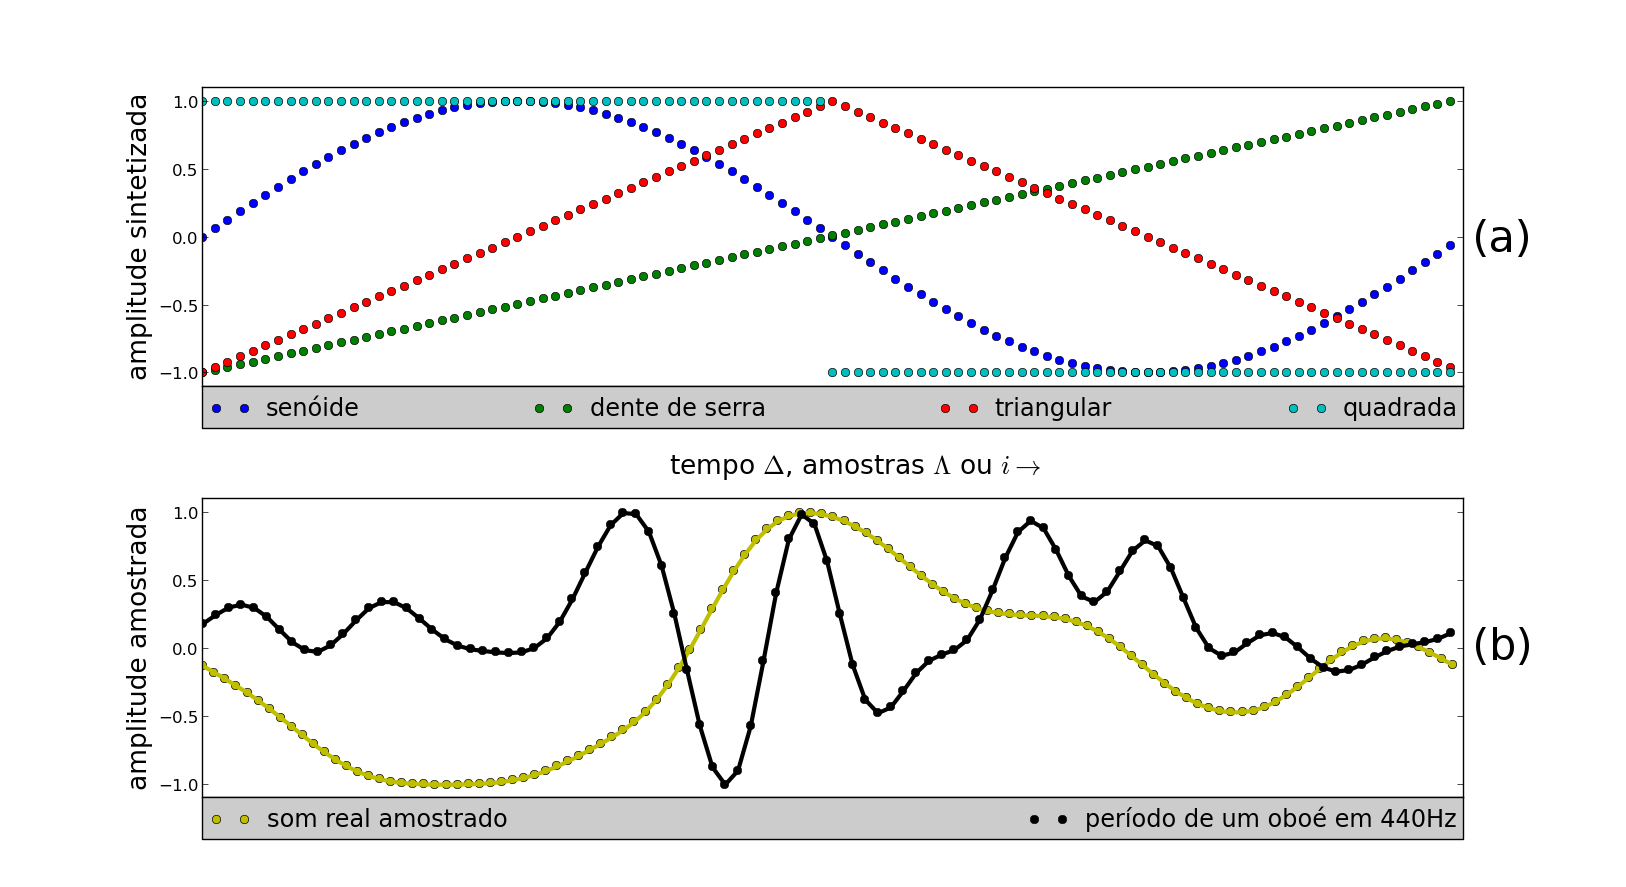
\includegraphics[width=\textwidth]{figuras/formasDeOnda6}
        \label{fig:formasDeOnda}
\end{figure}



A figura ~\ref{fig:formasDeOnda} apresenta
as formas de onda descritas nas equações ~\ref{senoide}, ~\ref{denteDeSerra}, ~\ref{triangular} e ~\ref{quadrada} para $\lambda_f=100$ (período
de $100$ amostras).
Se $t_a=44,1 kHz$, como no padrão PCM de Compact Disks, a onda possui frequência fundamental $f=\frac{f_a}{\lambda_f}=\frac{44100}{100} = 441 \; Herz $. Um lá\footnote{Um lá 4, logo acima do dó central, no segundo espaço do pentagrama na clave de sol comum.}, seja qual for a forma de onda dentre as artificiais apresentadas.

Estas formas de onda possuem usos especiais na música e seus espectros estão dispostos na figura ~\ref{fig:espectroDeOndas}. É importante notar as componentes isoladas e exatamente harmônicas dos espectros,
resultado de um período mantido fixo com exatidão. A senoide consiste de um nódulo único no espectro, frequência pura. A dente de serra é a única com a série harmônica completa (pares e ímpares). Já as ondas triangular e quadrada possuem as mesmas componentes espectrais, mas com decaimentos de $-12dB/oitava$ e $-6dB/oitava$.

\begin{figure}[h!]
    \centering
    \caption{Espectros das ondas sonoras musicais artificiais básicas}
        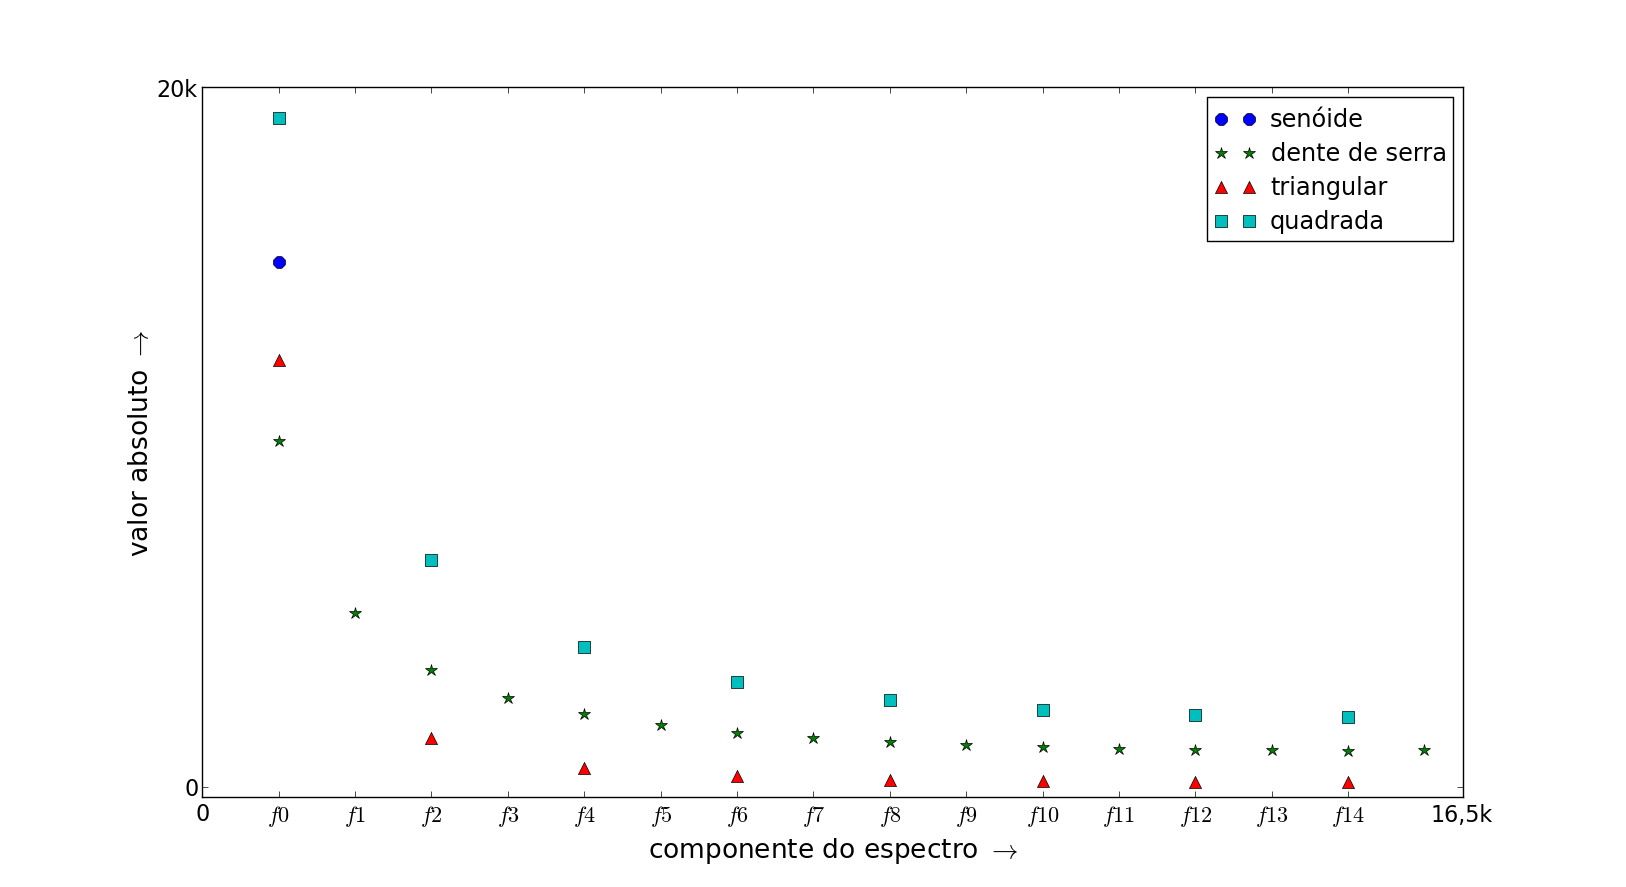
\includegraphics[width=\textwidth]{figuras/espectroDeOndas6}
        \label{fig:espectroDeOndas}
\end{figure}


O espectro harmônico é formado pelas frequências múltiplas da frequência fundamental $f_n=(n+1).f_0$.
Como nossa percepção segue uma progressão geométrica de frequências, o espectro possui notas diferentes da frequência fundamental. Além disso, o número de harmônicos será limitado pela frequência máxima $f_a/2$ (pelo Teorema de Nyquist). 

Musicalmente crucial aqui é internalizar que a presença de
energia\footnote{A energia total equivale à soma dos quadrados das amplitudes
(como as de pressao/voltagem no tempo), e.g. figura~\ref{fig:formasDeOnda}.
As componentes espectrais - e.g. figuras~\ref{fig:espectroDeOndas} e ~\ref{fig:espectroOboe} -
também podem ser elevadas ao quadrado para resultar em quantificação de energia e somam-se na energia total. As energias se equivalem pelo teorema de Parseval: $\frac{1}{\Lambda} . \sum_{k=0}^{\Lambda -1}c_k^2 = \sum_{i=0}^{\Lambda-1}t_i^2$.}
em uma componente de frequência $f_n$ na decomposição por fourier 
implica na presença de uma oscilação senoidal na constituição do som, puramente harmônica no som e naquela frequência $f_n$. Esta energia concentrada especificamente na frequência $f_n$ é separada
 pelo ouvido para adentrar em um nível cognitivo de processamento\footnote{Esta separação em frequência é realizada por diversas espécies através de mecanismos similares à cóclea humana~\cite{Roederer}.}.
  As componentes senoidais são geralmente as principais responsáveis pela qualidade chamada timbre e, caso não apresentem proporções harmônicas (relações de pequenos números), o som é percebido ruidoso, i.e. não são notas com frequência fundamental estabelecida unívocamente como um lá 4 ($440 Hz$) de nossos exemplos. Além disso, nossa noção de altura absoluta em um complexo sonoro é baseada na semelhança do espectro com a série harmônica~\cite{Roederer}.

No caso de uma forma de onda fixa (e de tamanho fixo), o espectro é sempre harmônico e estático. Fixada a frequência fundamental (inverso do comprimento da onda), cada forma de onda é composta de proporções específicas das componentes harmônicas e 
quanto maior a curvatura do trecho na forma de onda, maior a contribuição do trecho para a
concentração de energia nos harmônicos agudos.

Podemos ver isso claramente em sons reais. A onda rotulada como 'som real amostrado' na figura ~\ref{fig:formasDeOnda} é um período extraído de um som real relativamente comportado. Ele possuí $\lambda_f=114$ amostras\footnote{Caso também utilizado diretamente em $f_a=44,1kHz$, é um pouco mais grave que os $441 Hz$ das formas de onda artificiais $\frac{44100}{114}=385,84Hz$.}. A onda de oboé foi amostrada de um lá 4 também em $44,1kHz$.
O período escolhido para a amostragem é relativamente curto, com 98 amostras corresponde a 
uma frequência de $\frac{44100}{98}=450 Hz$. Pode-se perceber, através das curvaturas, o espectro rico em 
frequências agudas do oboé e o espectro mais grave do som real.

Note que, definindo $ R_i=\{ r_i \}_0^{\lambda_f-1}$ a sequência de amostras do som real da figura ~\ref{fig:formasDeOnda},
$R_i$ pode ser tomado como base para um som $T_i^f$ da seguinte forma: 

\begin{equation}\label{sampleandoFormaDeOnda}
     T^f_i=\{ t_i^f \}=\Bigl\{ r_{(i\,\%\lambda_{f})} \Bigr\}
\end{equation}

O som resultante possui o espectro momentâneo do som original. Por ser repetido de forma idêntica,
seu espectro é perfeitamente harmônico, sem os ruídos e variações típicas do fenômeno natural. Isso pode ser 
visto claramente na figura \ref{fig:espectroOboe} onde os espectros da nota original do oboé e de uma nota 
artificial - de mesma duração e cujas amostras consistem no mesmo período da figura ~\ref{fig:formasDeOnda} - estão dispostas juntamente. O espectro natural possui variações na frequência dos harmônicos, nas suas intensidades e uma quantidade de ruído. Já a nota cujo período foi amostrado possui espectro perfeitamente harmônico.



\begin{figure}[h!]
    \centering
    \caption{Espectros das ondas sonoras do oboé natural e de período amostrado}
        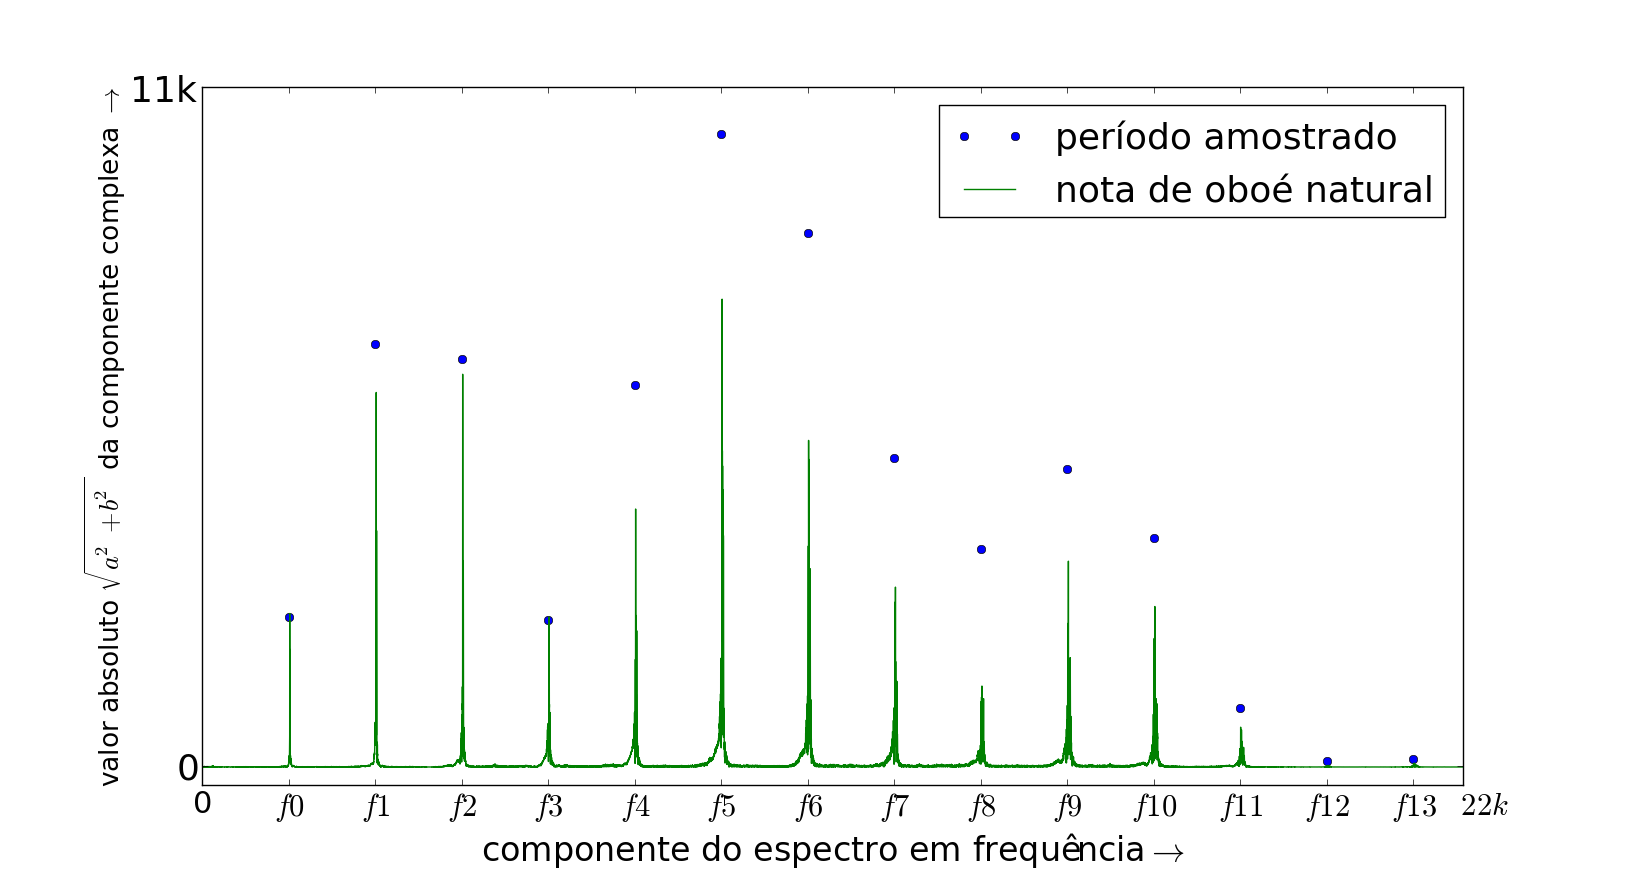
\includegraphics[width=\textwidth]{figuras/espectroOboeAmostradoNatural3}
        \label{fig:espectroOboe}
\end{figure}





\subsection{O espectro no som amostrado}
Além deste papel-chave na cognição (especialmente no timbre), a presença e comportamento destas componentes senoidais 
no som discretizado possui particularidades. Considere um sinal $T_i$ e sua decomposição de Fourier $\mathcal{F}\langle T_i\rangle=C_i=\{c_i\}_0^{\Lambda-1}$. Sabemos que a recomposição segue a conversão das componentes frequenciais em amostras temporais\footnote{Lembrando que o fator $\frac{1}{\Lambda}$ pode ser distribuído dentre a transformada e a reconstrução como preferir}:

 
\begin{equation}\label{recomposicaoFourier}
t_i = \frac{1}{\Lambda}\sum_{k=0}^{\Lambda-1}c_ke^{j \frac{2\pi k}{\Lambda} i } = \frac{1}{\Lambda}\sum_{k=0}^{\Lambda-1}(a_k+ j . b_k)\left[cos(w_k i) +j . sen(w_k i)\right]
\end{equation}

Onde $c_k = a_k + j . b_k$ pondera a amplitude e fase de cada frequência: $w_k=\frac{2\pi k}{\Lambda}$ em radianos ou $f_k=w_k\frac{f_a}{2\pi}=\frac{k.f_a}{\Lambda}$ em Herz (com atenção os respectivos limites em $\pi$ e em $\frac{f_a}{2}$). Nosso som possui amostras $t_i$ reais que resultam das contribuições de cada componente de frequência $w_k=\frac{2\pi k}{\Lambda}$ e cujo $c_k$ regula o módulo e a fase. A parte real da equação ~\ref{recomposicaoFourier} nos fornece a componente de forma mais clara:

\begin{equation}\label{moduloEfase}
\begin{split}
t_i& = \frac{1}{\Lambda}\sum_{k=0}^{\Lambda-1}\left[a_k cos(w_k i) -b_k sen(w_k i)\right] \\
   & = \frac{1}{\Lambda}\sum_{k=0}^{\Lambda-1}\sqrt{a_k^2 + b_k^2} \; cos\left[w_k i - tg^{-1}\left(\frac{b_k}{a_k}\right)\right]
\end{split}
\end{equation}

Podemos notar claramente pela equação ~\ref{moduloEfase} que o termo imaginário acrescenta uma fase à senoide real. Os termos imaginários $b_k$ da decomposição espectral por Fourier proporcionam a varredura de fase
 $[-\frac{\pi}{2},+\frac{\pi}{2}]$, basta observar o termo $tg^{-1}\left (\frac{b_k}{a_k}\right )$ que possui este contra-domínio. O sinal de $a_k$ especifica se estamos do lado direito ou esquerdo do circulo trigonométrico, completando a varredura completa de fase (os intervalos $[-\frac{\pi}{2},+\frac{\pi}{2}]$ e $[\frac{\pi}{2},\frac{3\pi}{2}]$ se justapõem em $2\pi$).


\begin{figure}[h!]
    \centering
    \caption{Oscilação de 2 amostras (frequência máxima em qualquer $f_a$)}
        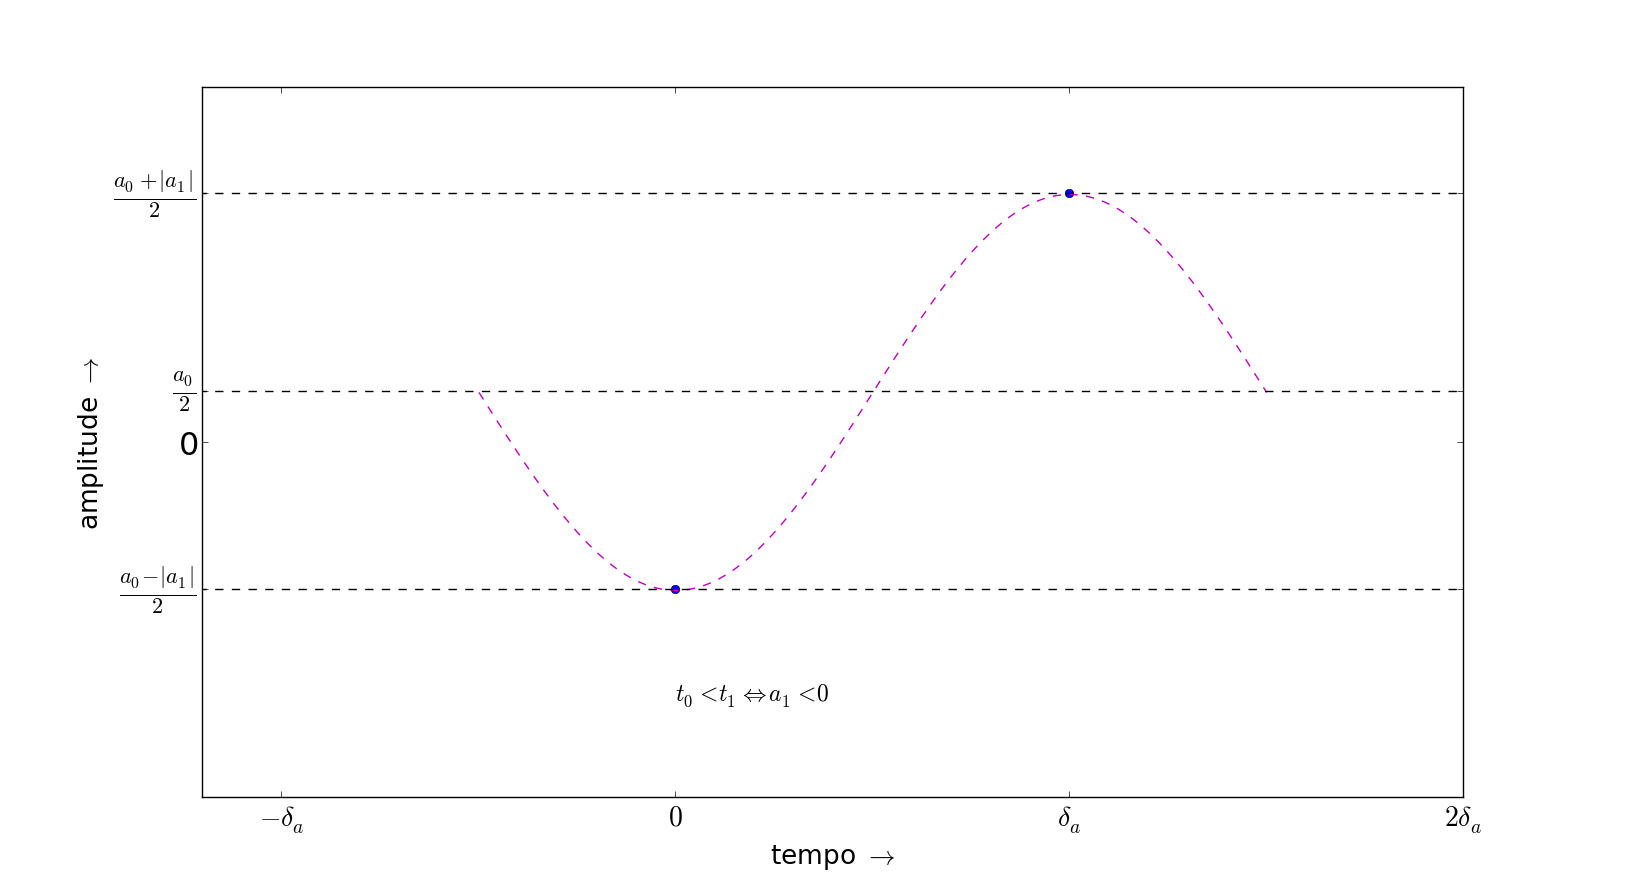
\includegraphics[width=\textwidth]{figuras/amostras2c__}
        \label{fig:amostras2}
\end{figure}

A figura ~\ref{fig:amostras2} exibe duas amostras e a componente espectral que contém. A decomposição de Fourier resulta neste caso em somente dois coeficientes $\{c_k=a_k-j.b_k\}_0^{\Lambda-1=1}$ relativos à frequências $\{f_k\}_0^1=\{w_k\frac{f_a}{2\pi}\}_0^1=\{k\frac{f_a}{\Lambda=2}\}_0^1=\{0,\frac{f_a}{2}=f_{\text{máx}}\}$
com energias $e_k=\frac{(c_k)^2}{\Lambda=2}$. O papel das amplitudes $a_k$ fica bem claro:
 $\frac{a_0}{2}$ é o deslocamento fixo\footnote{Chamado em vários contextos de \emph{bias} ou \emph{offset}.} e $\frac{a_1}{2}$ especifica a amplitude da oscilação em si, dada pela relação $f_k=k . \frac{f_a}{\Lambda=2}$.

Este caso é de especial importância pois o mínimo necessário para representar uma oscilação são 2 amostras e disso resulta a frequência de Nyquist $f_{\text{máx}}=\frac{f_a}{2}$. Esta é a frequência máxima presente em um som amostrado com $f_a$ amostras por segundo\footnote{Qualquer sinal amostrado possui esta característica, não somente o som digitalizado.}.

Vejamos o que acontece no caso de 3 amostras. Todas as sequências fixas $T_i$ de apenas 3 amostras também apresentam
somente 1 frequência, pois sua primeira harmônica usaria 1,5 amostras e ultrapassa o limite inferior de 2 amostras mínimas (a frequência da harmônica ultrapassaria a de Nyquist pois:  $\; \frac{2. f_a}{3} > \frac{f_a}{2} $). Se $\Lambda=3$, 
os coeficiêntes $\{c_k\}_0^{\Lambda-1=2}$ da decomposição por Fourier apresentam-se em 
3 componentes frequenciais. Uma delas é relativa à frequência zero ($c_0$), as outras duas ($c_1$ e $c_2$) contribuem de forma igual na reconstrução da senoide com $f=f_a/3$.

\begin{figure}[h!]
    \centering
    \caption{3 amostras apresentam uma única frequência}
        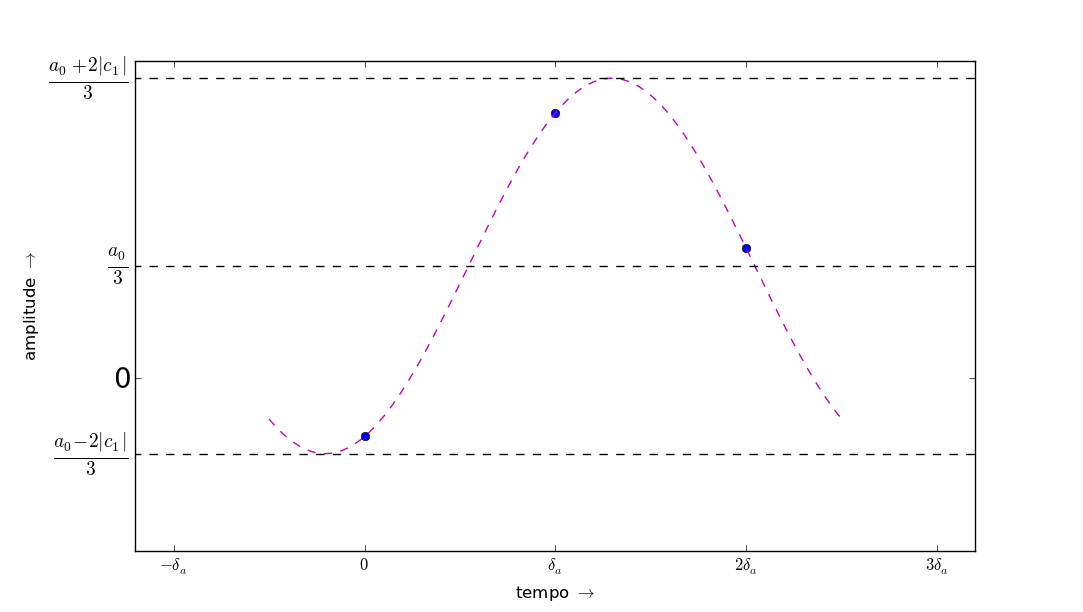
\includegraphics[width=\textwidth]{figuras/amostras3b}
        \label{fig:amostras3}
\end{figure}



Sempre que partimos de $\Lambda$ amostras reais $t_i$ resultamos em $\Lambda$ coeficientes complexos $c_k=a_k+j.b_k$. Os coeficientes $c_k$ se equivalem dois a dois\footnote{Parte real igual e imaginária com sinal trocado: $a_{k1}=a_{k2}$ e $b_{k1}=-b_{k2}$. Como consequência temos módulos iguais e fases com sinais opostos} correspondendo às frequências $f_k = k\frac{f_a}{\Lambda}, \; k \in \{0, ..., \left \lfloor \frac{\Lambda}{2} \right \rfloor \} $.
Quando $k> \frac{\Lambda}{2} $
a frequência $f_k$ é espelhada em $\frac{f_a}{2}$ da seguinte forma $f_k=\frac{f_a}{2} - (f_k-\frac{f_a}{2})=f_a-f_k=f_a - k\frac{f_a}{\Lambda}=(\Lambda-k)\frac{f_a}{\Lambda} \;\;\;\; \Rightarrow \;\;\;\; f_k\equiv f_{\Lambda-k} \; ,\;\; \forall \;\; k<\Lambda$. 

 
 O mesmo pode ser observado com 
 $w_k=f_k.\frac{2\pi}{f_a}$ e lembrando da periodicidade $2\pi$, que resulta em $w_k=-w_{\Lambda-k}$. Como o coseno é uma função par e a tangente inversa é impar, as componentes em $w_k$ e $w_{\Lambda-k}$ se somam na equação de reconstrução das amostras reais mostrada em ~\ref{recomposicaoFourier}.

  Dito de outra forma, em uma decomposição de $\Lambda$ amostras, as $\Lambda$ componentes frequenciais $\{c_i\}_0^{\Lambda-1}$ resultantes
   são equivalentes em pares.
   Excepcional excessão para $f_0$ e, no caso de $\Lambda$ ser par, de $f_{\Lambda/2}=f_{\text{máx}}=\frac{f_a}{2}$ , ambas as componentes são isoladas, i.e. não existe outra componente na frequência $f_0$ ou $f_{\Lambda/2}$ (se $\Lambda$ par) além dela mesma. 
Pois $f_{\Lambda/2}=f_{(\Lambda-\Lambda/2) = \Lambda/2}$ e $f_0=f_{(\Lambda-0)=\Lambda}=f_0$.

Além disso, estas duas frequências (a frequência zero e a frequência máxima) não são representadas com variação de fase e, portanto, são estritamente reais. Assim, podemos 
   concluir que o número $\tau$ de pares de coeficientes equivalentes é:

\begin{equation}\label{coefsPareados}
\tau = \frac{\Lambda - \Lambda \% 2}{2} +\Lambda \% 2 -1
\end{equation}

e resultam evidentes as equivalências ~\ref{equivalenciasFreqs}, ~\ref{equivalenciasModulos} e ~\ref{equivalenciasFases}:

\begin{equation}\label{equivalenciasFreqs}
f_{k}\equiv f_{\Lambda-k}\;, \;\; w_{k}=-w_{\Lambda-k}\;\;\;, \quad \;\; \forall \quad 1 \leq k \leq \tau  
\end{equation}

\begin{figure}[h!]
    \centering
    \caption{Componentes frequenciais em 4 amostras}
        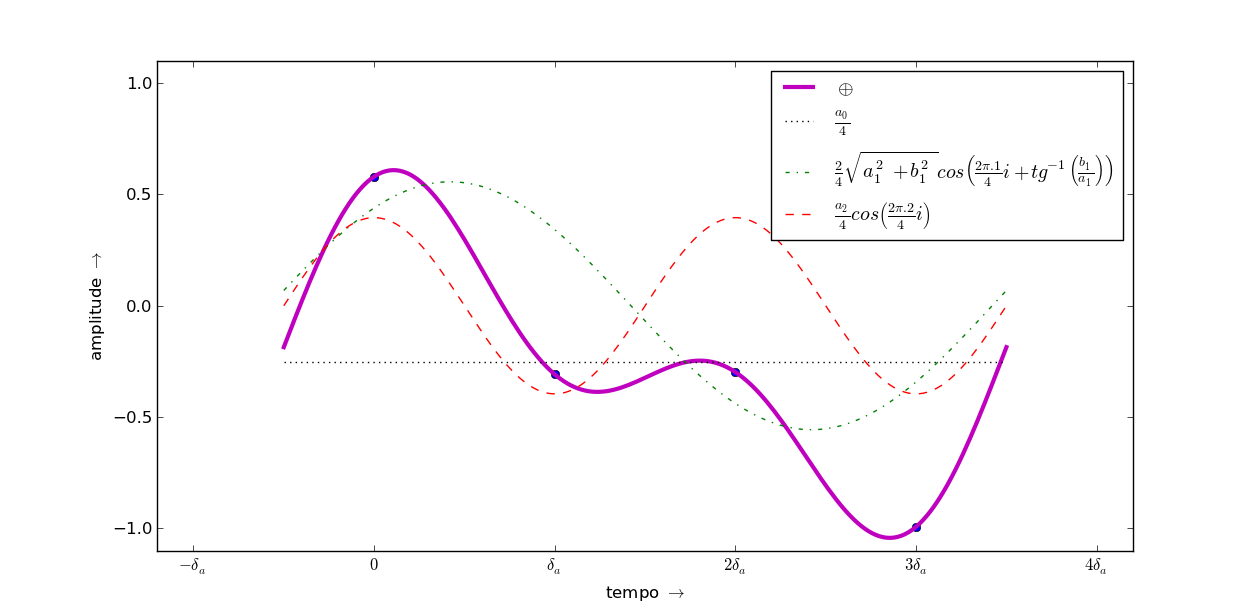
\includegraphics[width=\textwidth]{figuras/amostras4__}
        \label{fig:amostras4}
\end{figure}


Como $a_k = a_{\Lambda -k}\;\;$ e $\;\;b_k = - b_{\Lambda -k}$:

\begin{equation}\label{equivalenciasModulos}
\sqrt{a_k^2 + b_k^2} = \sqrt{a_{\Lambda - k}^2 + b_{\Lambda -k}^2} \;\;, \quad \;\; \forall \quad 1 \leq k \leq \tau  \\
\end{equation}

\begin{equation}\label{equivalenciasFases}
tg^{-1}\left(\frac{b_k}{a_k}\right)=-tg^{-1}\left(\frac{b_{\Lambda -k}}{a_{\Lambda - k}}\right)\;\;,\quad \;\; \forall \quad 1 \leq k \leq \tau
\end{equation}



Com $k \in \mathbb{N}$. A observação da equação de reconstrução para o sinal real ~\ref{moduloEfase} em conjunto com as equivalências dos módulos e fases ~\ref{equivalenciasModulos} e ~\ref{equivalenciasFases}, o número de coeficientes pareados \ref{coefsPareados} e equivalência de pares de frequências \ref{equivalenciasFreqs}
expõe o caso geral da combinação em fase das componentes em cada amostra $t_i$:

\begin{equation}
t_i = \frac{a_0}{\Lambda} + \frac{2}{\Lambda}\sum_{k=1}^{\tau}\sqrt{a_k^2 + b_k^2} \; cos\left[w_k i - tg^{-1}\left(\frac{b_k}{a_k}\right)\right]+ \frac{ a_{\Lambda/2}}{\Lambda}.(1-\Lambda\% 2)
\end{equation}

\begin{figure}[h!]
    \centering
    \caption{Formas de onda básicas em 4 amostras}
        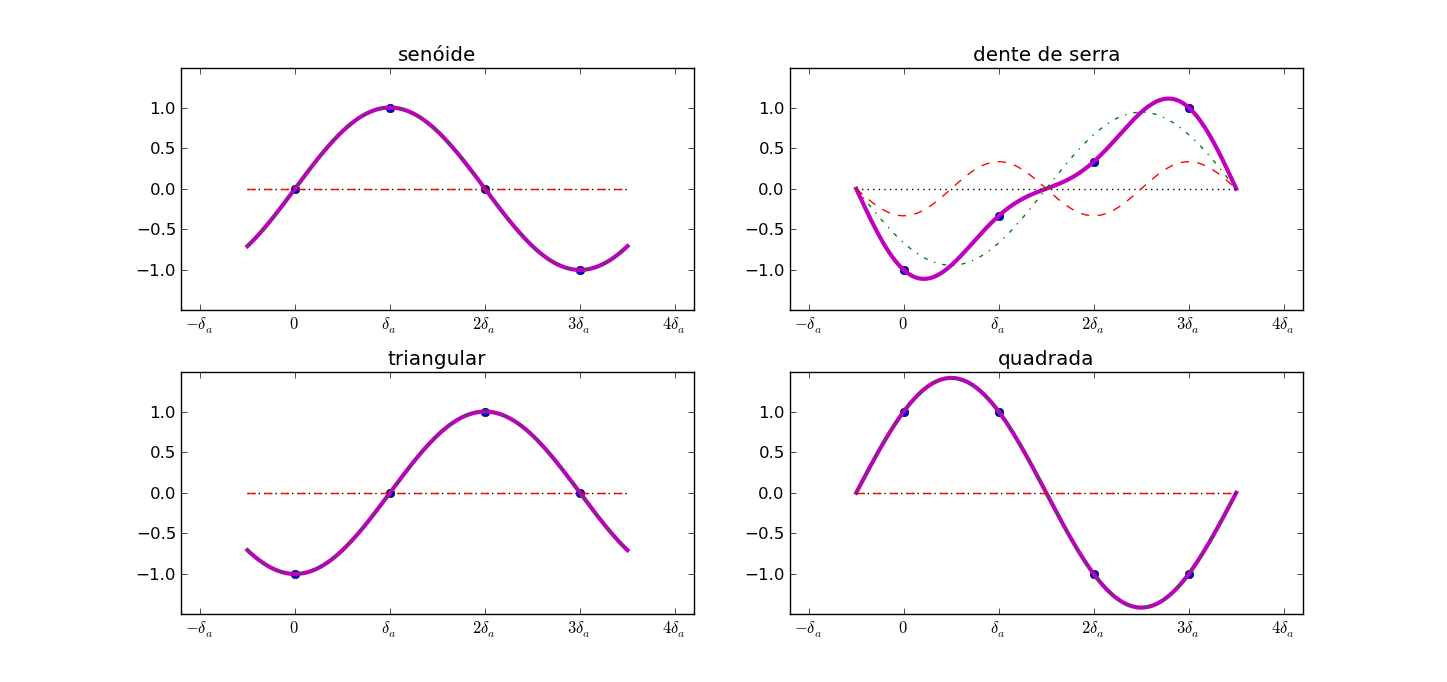
\includegraphics[width=\textwidth]{figuras/amostras4formas__}
        \label{fig:formas4}
\end{figure}


Assim, a exemplo da figura ~\ref{fig:amostras3}, a transformada de Fourier de 3 amostras possui 2 coeficientes frequenciais que possuem quantidades iguais de energia na mesma frequência.

Com 4 amostras, podemos representar 1 ou 2 frequências em proporções diferentes. A figura ~\ref{fig:amostras4} mostra uma 
forma de onda de 4 amostras e suas duas componentes. 
Note que as contribuições individuais se somam de fato na forma de onda 
original, e que as curvaturas maiores são fruto da frequência mais aguda
enquanto um deslocamento fixo da somatória das componentes é fruto
da componente na frequência zero.

A figura ~\ref{fig:formas4} explicita os harmônicos em 4 amostras nas formas de onda básicas das equações ~\ref{senoide}, ~\ref{denteDeSerra}, ~\ref{triangular} e ~\ref{quadrada} e figura ~\ref{fig:formasDeOnda}. Todas consistem em apenas 1 senoide, com excessão da dente de serra que possui os harmônicos pares.


A figura ~\ref{fig:amostras6} mostra uma decomposição senoidal para o caso de 6 amostras e a figura ~\ref{fig:formas6} decompõe as formas de onda básicas para o caso de 6 amostras.
 Note que neste caso de 6 amostras todas as ondas se diferenciam no espectro: as quadrada e triangular possuem as mesmas componentes, mas em proporções diferentes, já a dente de serra possui uma componente a mais.

\begin{figure}[h!]
    \centering
    \caption{Componentes frequenciais em 6 amostras}
        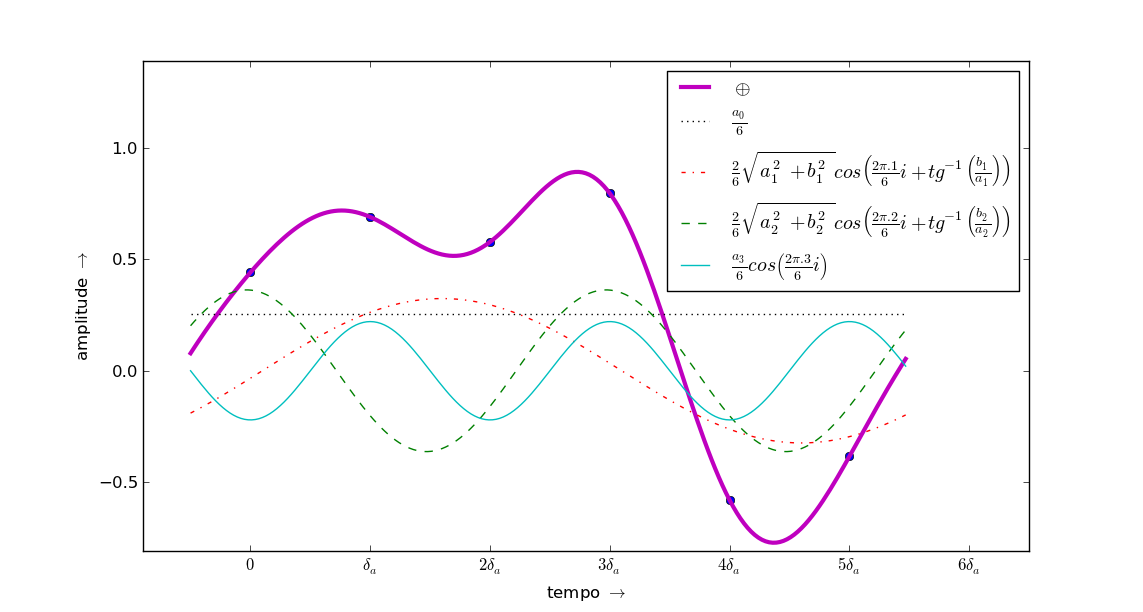
\includegraphics[width=\textwidth]{figuras/amostras6}
        \label{fig:amostras6}
\end{figure}

\begin{figure}[h!]
    \centering
    \caption{Formas de onda básicas em 6 amostras}
        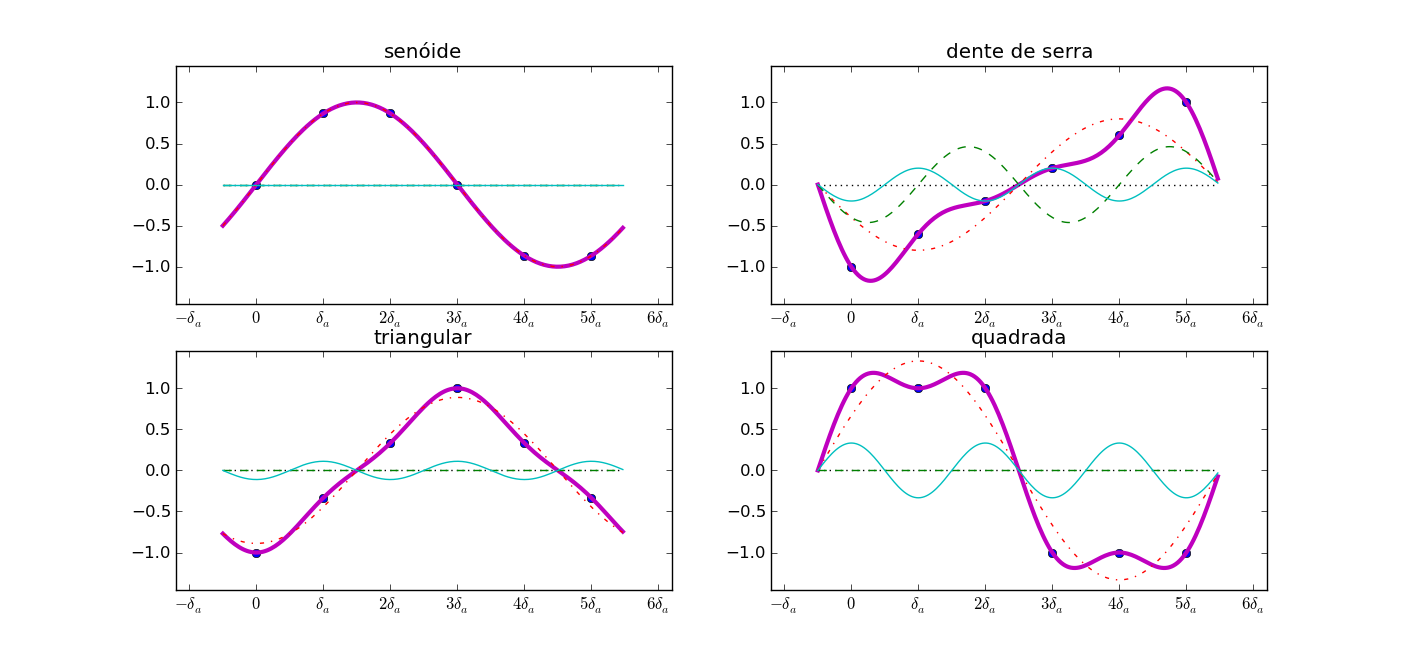
\includegraphics[width=\textwidth]{figuras/amostras6formas___}
        \label{fig:formas6}
\end{figure}

\subsection{Localização espacial}
Embora não seja uma das quatro qualidades básicas tradicionalmente elegidas para caracterizar uma nota musical,
a localização espacial é também importante para um som
pois este comumente é emitido por uma fonte localizada, como ocorre com um instrumento musical ou uma pessoa. Além disso, a espacialização é atributo bastante valorizado
 por audiófilos e pela indústria fonográfica~\cite{floEsp}.
Segundo a compreensão atual do fenômeno de percepção da localização espacial do som, nosso sistema nervoso utiliza
três informações: o atraso de chegada do som entre um ouvido e o outro, a diferença de intensidade do som direto em cada ouvido e a 
filtragem realizada pelo corpo, incluindo toráx, cabeça e orelhas~\cite{Roederer, hrtf, Heeger}.


\begin{figure}[h!]
    \centering
    \caption{Detecção de localização espacial de fonte sonora: DTI e DII}
        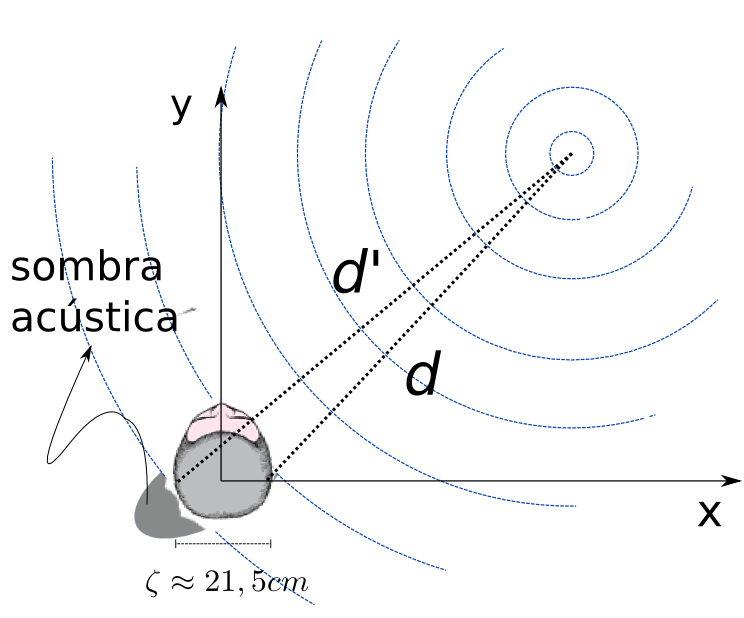
\includegraphics[width=.5\textwidth]{figuras/espacializacao___}
        \label{fig:spac}
\end{figure}



	Se consideradas somente as incidências diretas em cada ouvido, podemos dispor as diferenças de tempo e intensidade em equações simples. Dada a distância entre os ouvidos $\zeta\approx 21,5cm$,
um objeto localizado em $(x,y)$ conforme a figura~\ref{fig:spac}
está distante de cada ouvido:

\begin{equation}
\begin{split}
d & =\sqrt{\left (x-\frac{\zeta}{2} \right )^2+y^2} \\
d' & =\sqrt{\left (x+\frac{\zeta}{2} \right )^2 + y^2}
\end{split}
\end{equation}


e cálculos imediatos nos levam à DTI (Diferença de Tempo Interaural)\footnote{Constata-se que $\zeta \approx 21,5cm$ para um humano adulto.}:

\begin{equation}
DTI=\frac{d'-d}{v_{som\;no\;ar}\approx 343,2 }\quad \text{segundos}
\end{equation}

e à DII (Diferença de Intensidade Interaural):
\begin{equation}
DII=20\log_{10}\left (\frac{d'}{d}\right) \quad dBs
\end{equation}

Convertendo para amplitude temos $DII_a=\frac{d'}{d}$. A $DII_a$ pode
ser utilizada como constante multiplicativa do canal direito de um sinal sonoro estéreo ($\{t_i\}_0^{\Lambda -1}=\{DII_a . t_i'\}_0^{\Lambda -1}$). Pode-se utilizar a DII junto à DTI como adiantamento no tempo do canal direito com relação ao esquerdo, vínculo crucial para a percepção de localidade em sons graves e em sonoridades percussivas~\cite{Heeger}.
Considerando $\Lambda_{DTI}=\lfloor DTI . f_a \rfloor $, podemos escrever:

\begin{equation}
\begin{split}
\Lambda_{DTI} & = \left \lfloor \frac{d'-d}{343,2}  f_a \right \rfloor \\
DII_a & = \frac{d'}{d} \\
\{t_{(i+\Lambda_{DTI})}\}_{\Lambda_{DTI}}^{\Lambda+\Lambda_{DTI}-1} & =\{DII_a . t_i'\}_0^{\Lambda-1} \\
\{t_i\}_0^{\Lambda_{DTI}-1} & = 0
\end{split}
\end{equation}

Com $t_i$ o canal direito e $t_i'$ o canal esquerdo. Caso $\Lambda_{DTI} < 0 $, basta trocar $t_i$ por $t_i'$  e utilizar $\Lambda_{DTI}'= | \Lambda_{DTI} | $.

Embora consideravelmente simples até aqui, a localização espacial depende drasticamente de outras pistas. De forma canonica, resolvemos pelas
DTI e DII somente o ângulo horizontal (azimutal) $\theta$ dado por:

\begin{equation}
\theta=\tan^{-1}\left ( \frac{y}{ x }  \right )
\end{equation}

Mesmo assim, há dificuldades quando $\theta$ incinde sobre o chamado "cone de confusão" em que um mesmo par de especificações DTI, DII resultam de vários dos pontos 
do cone. Nestes pontos, a inferência do ângulo azimutal depende especialmente da filtragem atenuante nos agudos, pois a cabeça interfere um tanto mais nas ondas mecânicas agudas do que nas graves~\cite{Heeger,hrtf}. 

A figura~\ref{fig:spac} mostra esta sombra acústica do crânio, importante para a percepção do ângulo azimutal da fonte no cone de confusão. O cone em si não foi disposto na figura pois não é exatamente um cone e suas dimensões precisas não são especificadas na literatura~\cite{confCone}, mas pode ser entendido como um cone com o ápice no meio da cabeca e saindo por cada uma das orelhas.

Já a localização completa, incluindo distância e elevação da fonte sonora, é dada pela função de transferência de cabeça (HRTF - do inglês \emph{Head Related Transfer Function}~\cite{hrtf}. Exitem bases abertas e conhecidas de HRTF como \emph{CIPIC}~\cite{CIPIC} e podemos aplicar estas funções de transferência em um som por convolução (veja equação~\ref{eq:conv}). Estas funções de transferência mudam de acordo com o corpo do indivíduo e existem diversas técnicas para resultar em funções de transferência que sejam utilizáveis de forma mais universal~\cite{lazaSPA}. 


\subsection{A nota básica}\label{notaBasica}

Escolhamos $f$ tal que $f$ divida $f_a$  
 \footnote{Como apontado anteriormente, esta escolha facilita as demonstrações.
Transporemos esta limitação na próxima sessão.}. 
Uma sequência $T_i$ de amostras sonoras separadas por $\delta_a=1/f_a$ descreve uma nota musical de frequência $f$ Herz e duração $\Delta$ segundos se, e somente se, possuir a periodicidade $\lambda_f=f_a/f$
 e tamanho $\Lambda=\lfloor f_a . \Delta \rfloor $:

\begin{equation}
T_i^{f,\; \Delta}=\{t_{i \, \% \lambda_f} \}_0^{\Lambda-1}= \left \{t_{i \; \% \left( \frac{f_a}{f} \right) } \right \}_0^{\Lambda-1}
\end{equation}

Note que a nota por si só não especifica um timbre. Mesmo assim, faz-se necessária a escolha de uma forma de onda para que as amostras $t_i$ tenham um valor estabelecido individualmente. Um único período dentre as ondas básicas pode ser utilizado para a especificação da nota da seguinte forma:

seja $f$ a frequência da nota e escolhamos $f$ tal que $f$ divida $f_a$ (transporemos esta limitação na sessão seguinte). Assim, o inteiro $\lambda_f=\frac{f_a}{f}$ é o número de amostras do período. Temos que $L_i^{f,\, \delta_f} $ é
a sequência que descreve um período da onda $L_i^f \in \{S_i^f,Q_i^f,T_i^f,D_i^f,R_i^f \}$ de duração 
$\delta_f=1/f$ (ver equações ~\ref{senoide}, ~\ref{denteDeSerra}, ~\ref{triangular} e ~\ref{quadrada}; $R_i^f$ 
é uma onda real amostrada):

\begin{equation}\label{periodoUnico}
L_i^{f , \delta_f } = \{ l_i^f \}_0^{\delta_f . f_a -1}=\{ l_i^f \}_0^{\lambda_f-1}
\end{equation}

Então a sequência $T_i$ consistirá em uma nota de duração $\Delta$ e frequência $f$ se:

\begin{equation}
T_i^{f,\; \Delta}=\{t_i^f\}_0^{\lfloor f_a . \Delta \rfloor -1}=\left \{ l^f_{i\,\%\left(\frac{f_a}{f}\right)} \right \}_0^{\Lambda-1}
\end{equation}


\subsection{Usos musicais}


Em posse da nota básica, podemos montar estruturas musicais com
sequências destas partículas. Caso somemos $N$ sequências ($T_{k,i}=\{t_{k,i}\}, \;\; k \in 0...N-1$) de mesmo tamanho, seus conteúdos espectrais serão sobrepostos e a isso damos o nome de mixagem:

\begin{equation}\label{eq:mixagem}
\{t_i\}=\left \{ \sum_{k=0}^{N-1}t_{k,i} \right \}
\end{equation}

\begin{figure}[h!]
    \centering
    \caption{Mixagem de três sequências sonoras}
        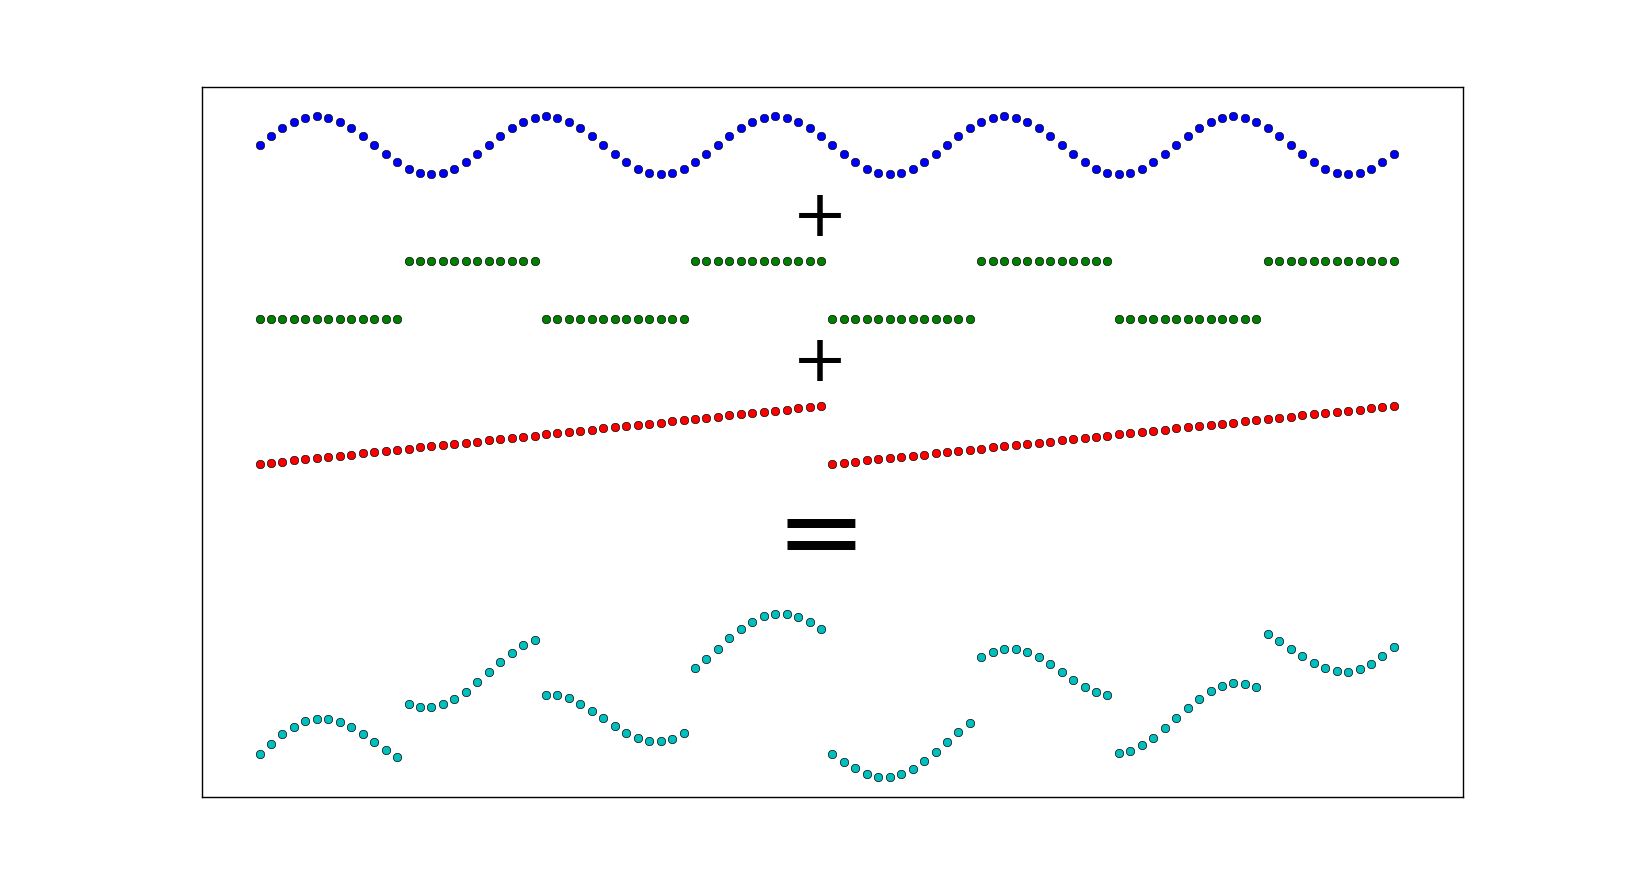
\includegraphics[width=\textwidth]{figuras/mixagem}
        \label{fig:mixagem}
\end{figure}


Ilustramos na figura~\ref{fig:mixagem} este processo de superposição de ondas sonoras discretizadas\footnote{A figura dispõe 100 amostras, de onde podemos concluir que, se $f_a=44,1kHz$, as frequências da dente de serra, da onda quadrada e da senoide são,
respectivamente, $\frac{f_a}{50}=882Hz$, $\frac{f_a}{25}=1764Hz$ e $\frac{f_a}{20}=2205Hz$. A duração do trecho é bastante curto $\frac{f_a=44,1kHz}{100} \approx 2 \text{ milisegundos}$.}.
 As notas mixadas são em grande parte separadas pelo ouvido por leis físicas de ressonância e pelo sistema nervoso~\cite{Roederer}.

Pode-se completar com zeros para somar sequências de tamanhos diferentes. O resultado da mixagem de notas musicais é a harmonia musical, cujos intervalos entre as frequências e os acordes de notas simultâneas regem aspectos subjetivos e abstratos da música e sua apreciação~\cite{Harmonia}. 

As sequências podem também ser concatenadas no tempo. Caso as sequências $\{t_{k,i}\}_0^{\Lambda_k-1}$ de tamanhos $\Lambda_k$  representem $k$ notas musicais, sua concatenação em uma única sequência $T_i$ resultará em uma sequência musical simples ou melodia:

\begin{equation}\label{eq:concatenacao}
\{t_i\}_0^{\sum\Delta_k-1}=\{t_{l,i}\}_0^{\sum\Delta_k-1}, \;\; l\text{ menor inteiro } : \quad \Lambda_l > i -\sum_{j=0}^{l-1}\Lambda_j
\end{equation}

Este mecanismo é demonstrado de forma ilustrativa na figura~\ref{fig:concatenacao} com as mesmas sequências utilizadas na figura ~\ref{fig:mixagem}.
 As sequências são curtas para as taxas de amostragem usuais (cerca de $7$ milisegundos ao total se $f_a=44,1kHz$), mas pode-se observar de forma explícita a concatenação de sequências sonoras e o exemplo é real (cada nota tem a duração maior que $100ms$ se $f_a<1kHz$).

\begin{figure}[h!]
    \centering
    \caption{Concatenação de três sequências sonoras}
        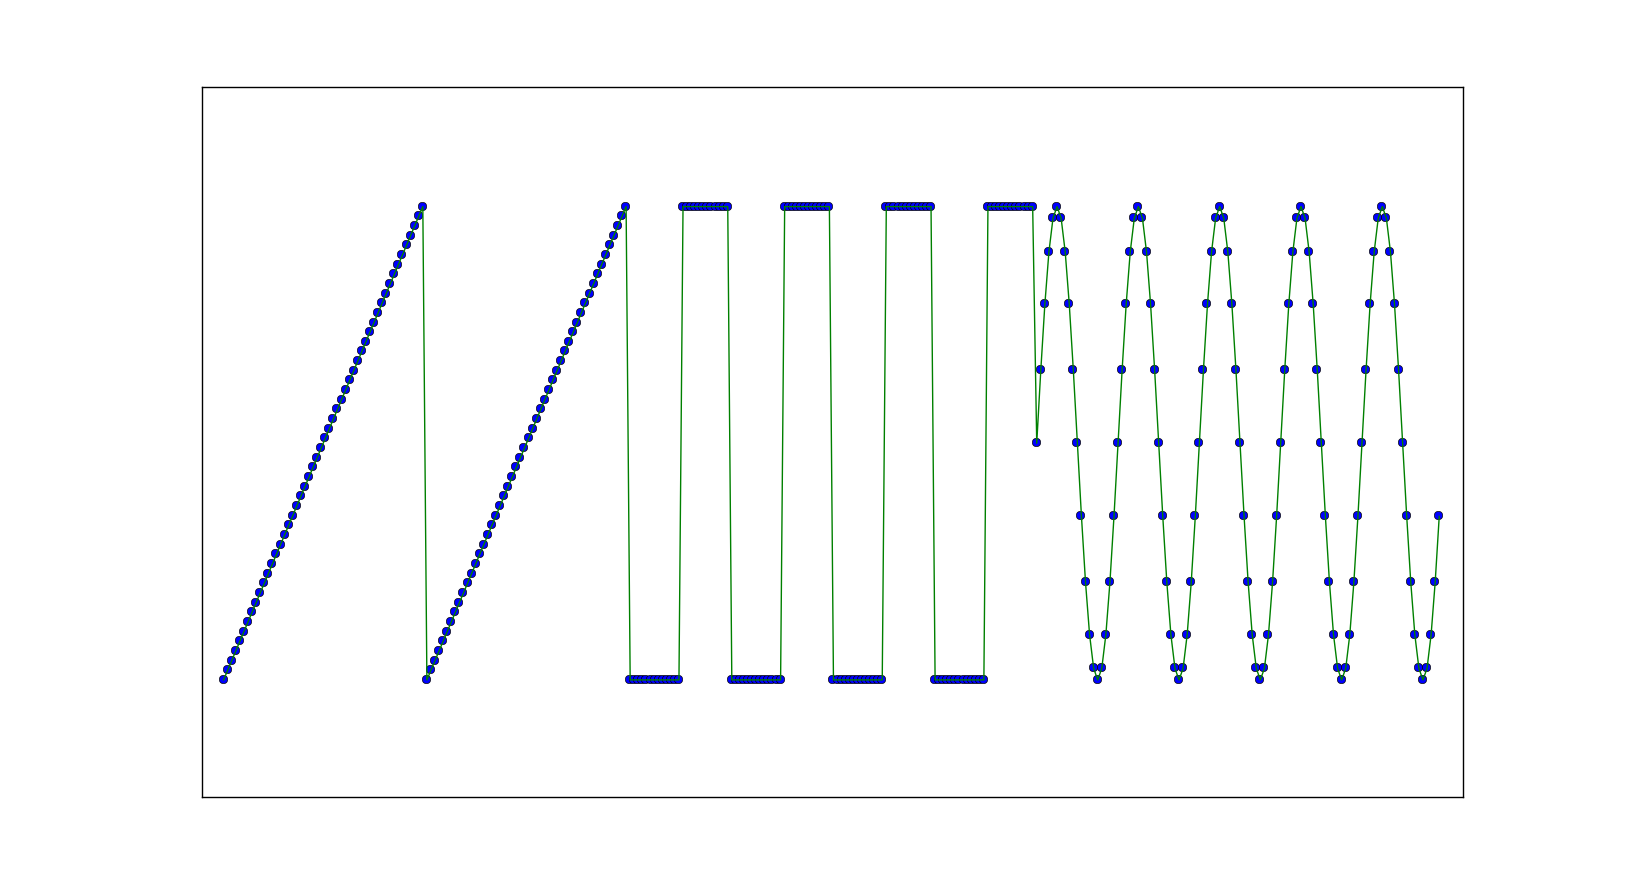
\includegraphics[width=\textwidth]{figuras/concatenacao}
        \label{fig:concatenacao}
\end{figure}

A montagem musical \emph{reduced-fi} demonstra de forma isolada este uso de justaposição temporal das notas, resultando em uma peça homofônica. O princípio vertical está demonstrado nos \emph{quadros sonoros}, sons estáticos com espectros peculiares. Ambas as peças estão em código Python no APÊNDICE~\ref{cap:codigoPecas} e podem ser escutadas e vizualizadas nos links~\cite{reduced-fi} e~\cite{quadros}.

Com isso estabelecemos nossa nota musical básica no som digital. Trabalharemos a seguir estas unidades, a evolução temporal de seus conteúdos e desenvolveremos as notas musicais com parâmetros que evoluem no tempo, como glissandos e envoltórias. 
A filtragem de componentes e os ruídos finalizam sobre a constituição da nota musical como unidade isolada. A estruturação musical destas notas é então abordada do ponto de vista das estruturas fora do tempo (como as escalas), trajetórias cíclicas ou que convirjam ou divirjam.

\clearpage

\section{Variações na nota musical básica}\label{varInternas}

Nossa nota musical digital básica está bem definida com os parâmetros:
duração, altura, intensidade (volume) e timbre. Esta é uma modelagem
útil e paradigmática, mas não esgota o que entendemos por
uma nota musical.

Em primeiro lugar, as características da nota se modificam no decorrer
da própria nota, i.e. em uma nota real os parâmetros
não são absolutamente fixos~\cite{Chowning}. Por exemplo, em uma nota de piano
de 3 segundos, a intensidade tem início abrupto e decaimento progressivo
além de variações do espectro instantâneo, com harmônicos que
decaem antes dos outros e alguns que aparecem com o tempo.
Estas variações não são obrigatórias e sim orientações da
síntese sonora para usos musicais pois é como os sons
se apresentam na natureza\footnote{A regra de ouro
aqui é: para que um som isolado disperte interesse
por si só, faça como que tenha variações internas~\cite{Roederer}.}. 

Explorar todas as formas pelas quais estas variações ocorrem está fora
do escopo de qualquer trabalho dada a considerável sensibilidade do ouvido humano
e a complexidade da nossa cognição sonora. Desta forma, apontaremos
recursos primários para estas variações das características na nossa nota
básica.

Iniciaremos com uma técnica que não resulta propriamente
em variações internas da nota, mas simplificará esta exposição
sem restringir o escopo, além de ser um notável recurso de otimização
computacional.



\subsection{Tabela de busca}

Mais conhecido pelo termo em inglês, a \emph{Lookup Table} (ou simplesmente
LUT), é um procedimento simples que consiste em criar uma tabela
de referência e coletar as amostras desta tabela segundo a 
necessidade\footnote{Em contraposição ao cálculo das amostras individuais
de forma analítica e permitindo o uso de funções sem possibilidade de cálculo direto
(por serem amostras recolhidas diretamente de algum fenômeno natural, por exemplo).}. Em nosso caso, usaremos tabelas de busca para os
sons criados, as notas. Assim, estas tabelas são unidimensionais e com
valores reais. Além disso, a tabela consiste nas amostras
de um período de onda, que usamos para sintetizar períodos
de tamanhos diferentes, resultando em frequências diferentes.

\begin{figure}[h!]
    \centering
    \caption{Lookup Table}
        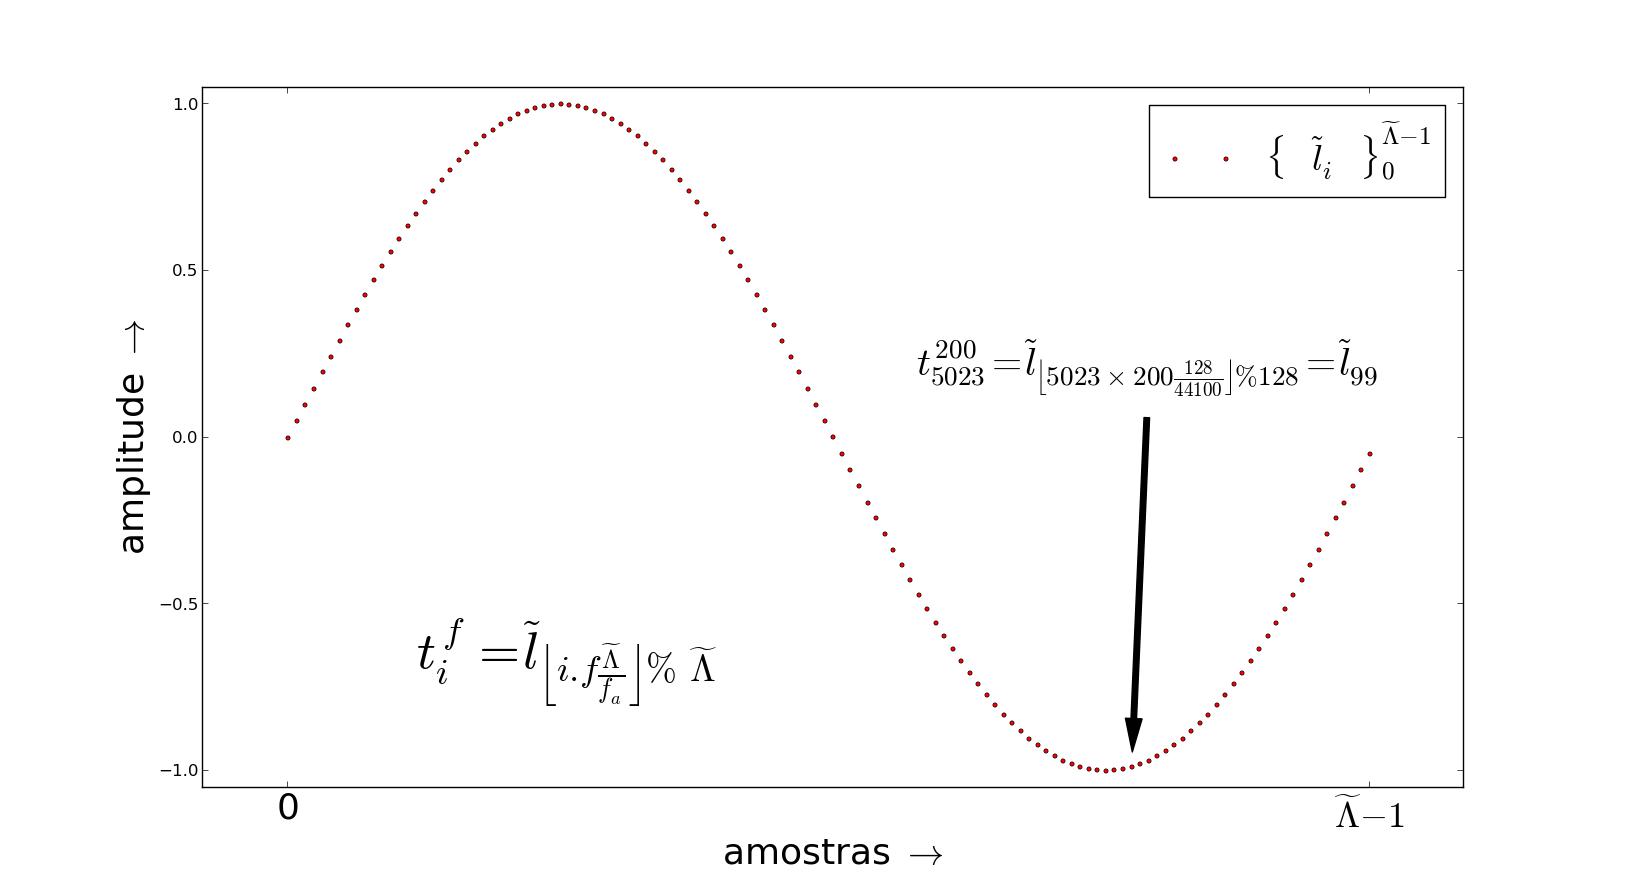
\includegraphics[width=\textwidth]{figuras/lut}
        \label{fig:lut}
\end{figure}

O procedimento de busca em tabelas é visto geralmente como um
artifício de otimização. Na música seu uso transcende este
primeiro, facilitando as operações e permitindo que um único
período de onda possa ser usado para sintetizar sons em toda a banda
de frequências audíveis, qualquer que seja a forma de onda amostrada.

Descrevemos esta busca. Seja $\widetilde{\Lambda}$ o tamanho 
da tabela e $\widetilde{L_i} = \{ \widetilde{l}_i \}_0^{\widetilde{\Lambda} -1}$ a tabela de elementos $\widetilde{l_i}$ de um
período de onda qualquer (veja equação ~\ref{periodoUnico}). Uma sequência
$T_i^{f,\,\Delta}$ com amostras de um som de frequência $f$ e duração $\Delta$
pode ser feita a partir de $\widetilde{L_i}$ da seguinte forma:

\begin{equation}
T_i^{f,\,\Delta}=\left\{t_i^f\right\}_0^{\lfloor \, f_a . \Delta \, \rfloor -1} = \left\{ \, \widetilde{l}_{\gamma_i \% \widetilde{\Lambda} }\, \right\}_{0}^{\Lambda-1}\; , \quad \text{onde} \;\; \gamma_i = \left \lfloor i . f \frac{ \widetilde{\Lambda}}{f_a} \right \rfloor  
\end{equation}

Ou seja, dada a tabela de busca, basta termos a sequência de índices corretos
para sintetizar o som em qualquer frequência. Dispomos graficamente
o procedimento de LUT na figura~\ref{fig:lut} onde calculamos explicitamente
também uma amostra de $\{t_i\}$ a partir de $\{\widetilde{l}_i\}$ para uma frequência
de $f=200Hz$, $\widetilde{\Lambda}=128$ e considerada a taxa de amostragem em $f_a=44.1kHz$.


Para o cálculo do inteiro $\gamma_i$, convencionamos
atribuir a ele o maior inteiro menor que $i.f\frac{\widetilde{\Lambda}}{f_a}$.
Esta aproximação introduz um ruído, mas conseguimos que este ruído seja desprezível
mesmo se o tomarmos como o maior inteiro acima da multiplicação
ou se arredondarmos por outros métodos. Além disso, para fins de síntese, em $f_a=44.1 kHz$
 o padrão é usar $\widetilde{\Lambda} = 1024$ amostras, pois já não gera ruído
 relevante no espectro audível~\cite{Geiger}.

 A expressão que define a variável $\gamma_i$ pode ser facilmente compreendida da
 seguinte forma: a variável $i$ é acrescida de $f_a$ em $1$ segundo (pela
 definição de $f_a$ e $i$, pois temos $f_a$ amostras $t_i$ em $1$ segundo). Caso a dividamos por $f_a$, teremos $\frac{i}{f_a}$,
fração esta que é acrescida de $1$ a cada $1$ segundo. Multiplicado pelo comprimento da
 tabela $\widetilde{\Lambda}$, teremos $i \frac{\widetilde{\Lambda}}{f_a}$
 que resulta na varredura completa da tabela $\widetilde{L_i}$ em 
 1 segundo com o acréscimo de $\widetilde{\Lambda}$ em $1$ segundo. Por fim,
 se multiplicarmos pela frequência $f$ que queremos, teremos $i . f \frac{\widetilde{\Lambda}}{f_a}$
 que resulta em $f$ varreduras completas da tabela $\widetilde{L_i}$ em $1$ segundo, i.e. a sequência
 resultante apresenta a frequência fundamental $f$.

Importantes considerações: $f$ é qualquer, só há limitantes nas frequências
graves quando o tamanho da tabela $\widetilde{\Lambda}$ não é suficientemente grande para a taxa de amostragem
$f_a$. O procedimento de busca em tabela
é computacionalmente bastante barato, substituindo cálculos por buscas simples (por isso geralmente
é entendido como um processo de otimização). Salvo quando assinalado,
no texto que segue usaremos este procedimento para todos os casos cabíveis pois
simplifica diversas rotinas e é computacionalmente coerente.

O uso de LUTs é bastante difundido nas implementações computacionais
voltadas para música e para um uso clássico que explora com ênfase
as LUTs na síntese sonora musical, recomendamos procurar pela chamada 
\emph{Wavetable Synthesis} que consiste em várias LUTs utilizadas em 
conjunto através da mixagem para gerar uma nota musical quasi-periódica~\cite{Cook,Wavetable}.


\subsection{Variações incrementais de frequência e intensidade}

Segundo revela a lei de Weber e Fechner, nossa percepção tem uma relação logarítmica com
o estímulo que a causa~\cite{Weber-Fechner}. Em outras palavras, um estímulo em progressão exponencial
é percebido como linear. Mesmo assim, dado o uso, explicitaremos também a variação
linear e começaremos descrevendo esta por razões didáticas.

Em uma nota de duração $\Delta = \frac{\Lambda}{f_a}$, a frequência $f=f_i$ varia de $f_0$ até $f_{\Lambda -1}$
linearmente. Podemos então escrever que:

\begin{equation}\label{freqLinear}
f_i=f_0 + (f_{\Lambda-1}-f_0)\frac{i}{\Lambda-1} \quad ,\quad \quad i \;\in\; \mathbb{N}, \quad i \;\in\; [0,\Lambda-1]
\end{equation}

\begin{equation}\label{indiceLinear}
\Delta_{\gamma_i}=f_i\frac{\widetilde{\Lambda}}{f_a} \quad \Rightarrow \quad \gamma_i=\left \lfloor \sum_{j=0}^{i} f_j\frac{\widetilde{\Lambda}}{f_a} \right \rfloor   =\left \lfloor \sum_{j=0}^{i} \frac{\widetilde{\Lambda}}{f_a} \left [f_0 + (f_{\Lambda-1}-f_0)\frac{j}{\Lambda-1} \right ] \right \rfloor 
\end{equation}

\begin{equation}\label{serieAmostralLin}
\left\{t_i^{\;\overline{f_0,\, f_{\Lambda-1}}}\right\}_0^{\Lambda-1}=\left\{\,\widetilde{l}_{\gamma_i \% \widetilde{\Lambda}}\,\right\}_0^{\Lambda-1}
\end{equation}

Onde $\Delta_{\gamma_i}=f_i\frac{\widetilde{\Lambda}}{f_a}$ é o incremento da LUT entre duas amostras dada a frequência do som na primeira amostra.

Desta forma, podemos calcular os elementos $t_i^{\;\overline{f_0,f_{\Lambda-1}}}$
com base no período $\{\widetilde{l}_i\}_0^{\Lambda-1}$.

As equações \ref{freqLinear}, \ref{indiceLinear} e \ref{serieAmostralLin} são relativas à progressão linear
da frequência. Como assinalado para o caso geral, também aqui
uma progressão de frequência
\emph{percebida} como linear segue uma progressão exponencial\footnote{Ou,
dito ainda de outra forma, uma progressão geométrica da frequência
é percebido como uma progressão aritmética de alturas.}.

Fazendo a varredura com $i$
de $0$ até $\Lambda-1$, podemos dizer que: $f_i=f_0 . 2^{\frac{i}{\Lambda-1} n_8}$ onde 
$n_8=\log_2\frac{f_{\Lambda-1}}{f_0}$ é o número de oitavas entre $f_0$ e $f_{\Lambda-1}$.
De forma que $f_i=f_0 . 2^{\frac{i}{\Lambda-1}\log_2\frac{f_{\Lambda-1}}{f_0}}=
f_0 . 2^{\log_2\left ( \frac{f_{\Lambda-1}}{f_0} \right )^{\frac{i}{\Lambda-1}}}=
f_0 \left ( \frac{f_{\Lambda-1}}{f_0} \right ) ^{\frac{i}{\Lambda -1}}$. Portanto,
nossas equações de referência para a síntese de transições de frequência tidas como
lineares pelo ouvido são:

\begin{equation}
f_i=f_0 \left ( \frac{f_{\Lambda-1}}{f_0} \right ) ^{\frac{i}{\Lambda -1}}
\end{equation}

\begin{equation}\label{indiceExponencial}
\Delta_{\gamma_i}=f_i\frac{\widetilde{\Lambda}}{f_a} \quad \Rightarrow \quad \gamma_i=\left \lfloor \sum_{j=0}^{i} f_j\frac{\widetilde{\Lambda}}{f_a} \right \rfloor   =\left \lfloor \sum_{j=0}^{i} f_0 \frac{\widetilde{\Lambda}}{f_a} \left ( \frac{f_{\Lambda-1}}{f_0} \right ) ^{\frac{j}{\Lambda -1}} \right \rfloor
\end{equation}

\begin{equation}\label{serieAmostralLog}
\left\{t_i^{\;\overline{f_0,\,f_{\Lambda-1}}}\right\}_0^{\Lambda-1}=\left\{\,\widetilde{l}_{\gamma_i \% \widetilde{\Lambda}}\,\right\}_0^{\Lambda-1}
\end{equation}

Onde usamos a equação \ref{indiceExponencial} para calcular a sequência $\{\gamma_i\}_0^{\Lambda-1}$ de índices para para
serem buscados na nossa tabela que contém um único período da forma de onda representado em uma sequência de $\widetilde{\Lambda}$
pontos igualmente espaçados (amostras).
Isso é explicitado na equação ~\ref{serieAmostralLog}, onde estabelecemos a relação
 $t_i^{\;\overline{f_0,f_{\Lambda-1}}}=\widetilde{l}_{\gamma_i \% \widetilde{\Lambda}}$.
Note que a equação \ref{serieAmostralLog} se mantém (é idêntica à equação \ref{serieAmostralLin}).

\begin{figure}[h!]
    \centering
    \caption{Transições de intensidade para diferentes valores de $\alpha$ (veja equações~\ref{seqAmp} e ~\ref{transAmp})}
        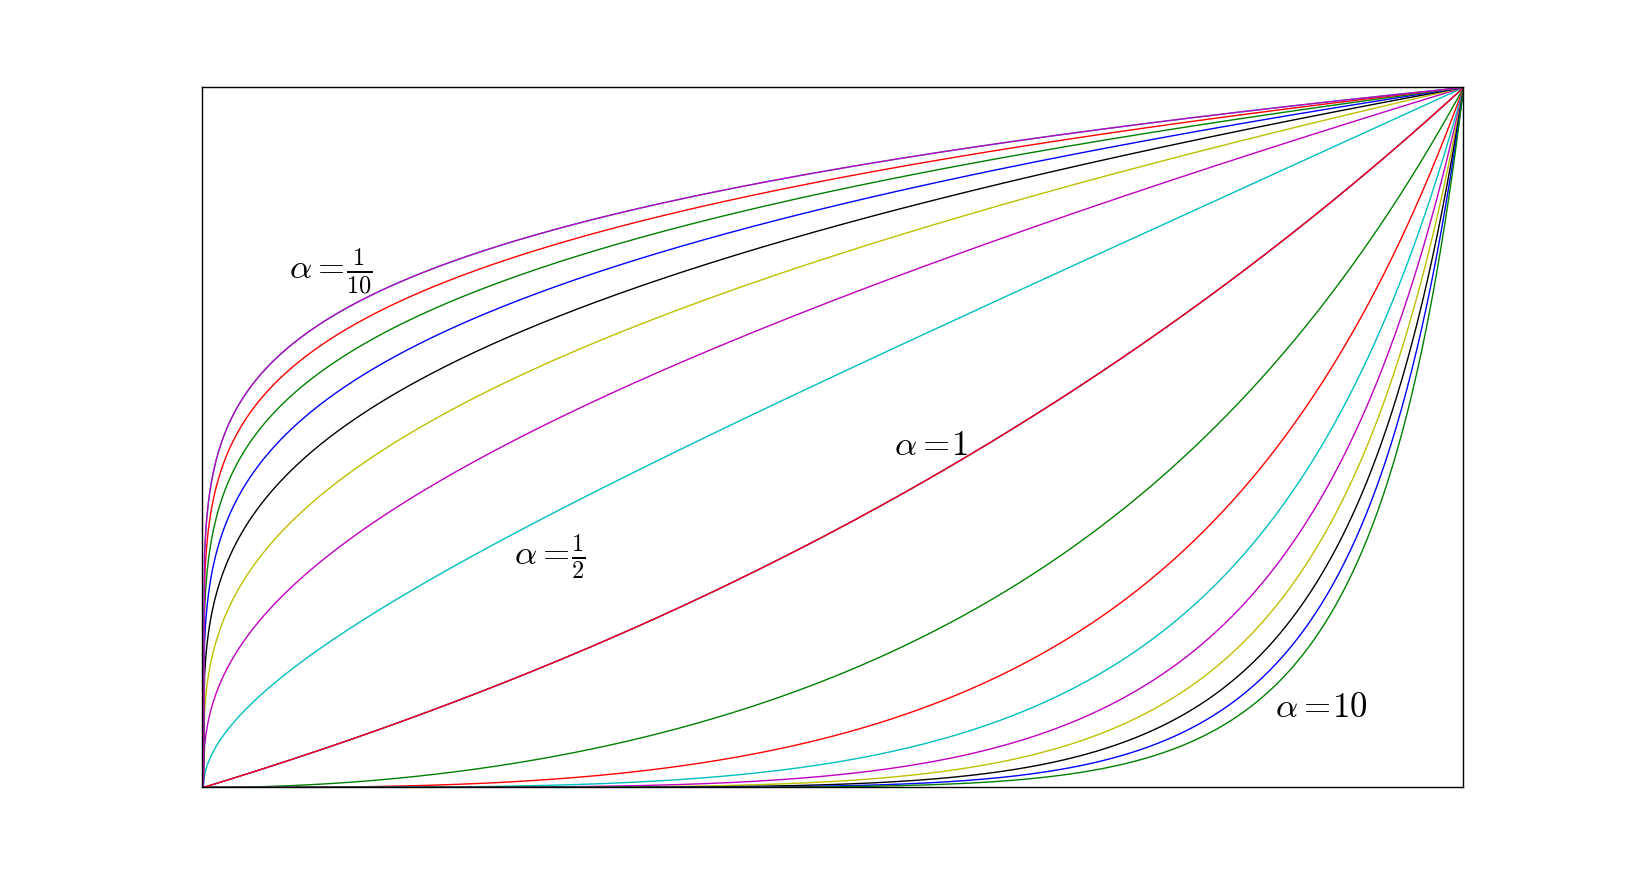
\includegraphics[width=\textwidth]{figuras/transicao}
        \label{fig:transicao}
\end{figure}


O termo $\frac{i}{\Lambda-1}$ varre o intervalo $[0,1]$ e podemos elevá-lo a uma potência
para que o início da transição seja mais suave ou mais abrupto (compensado pelo final
da transição). Este procedimento é mais comum para o caso de variações de volume através da energia
da onda vibratória\footnote{O alteração do volume pode ocorrer por diversas características como
a reverberação, a concentração de harmônicos agudos e a energia. Para nós, neste ponto da exposição,
a mais facilmente controlada é a energia da onda (veja equação ~\ref{potencia}) e a energia também pode variar de diferentes formas.
Uma forma mais simples e conveniente é a variar a amplitude pela multiplicação da sequência toda
por algum número real. A variação de energia sem variação de
amplitude é comumente chamada de \emph{compressão sonora} e é muito útil e corriqueira na prática
de produção musical atual~\cite{compressao}.}. Podemos obter este resultado multiplicando a sequência original
(seja ela gerada ou pré-estabelecida) pela sequência $a_{\Lambda-1}^{\left( \frac{i}{\Lambda-1} \right )^\alpha}$
onde $\alpha$ é o coeficiente citado e $a_{\Lambda-1}$ é fração da amplitude original que se visa atingir ao final da transição.

Assim, para variações de amplitude, aplicamos as seguintes fórmulas:

\begin{equation}\label{seqAmp}
\{a_i\}_0^{\Lambda-1}=\left \{ a_0 \left ( \frac{a_{\Lambda-1}}{a_0} \right )^{\left ( \frac{i}{\Lambda-1} \right )^\alpha} \right \}_0^{\Lambda-1}=\left \{ \left ( {a_{\Lambda-1}} \right )^{\left ( \frac{i}{\Lambda-1} \right )^\alpha} \right \}_0^{\Lambda-1} \text{ com } a_0=1
\end{equation}

\begin{equation}\label{transAmp}
T_i^{'}=T_i \odot A_i = \{t_i . a_i\}_0^{\Lambda-1}=\left \{ t_i . (a_{\Lambda-1} )^{\left ( \frac{i}{\Lambda-1} \right )^\alpha} \right \}_0^{\Lambda-1}
\end{equation}

Nosso intuito aqui é modificar a amplitude de um sinal original, seja qual for ele. Desta forma, tomamos
$a_0=1$ para iniciar a nova sequência com a amplitude original e então ir modificando com o decorrer das amostras.
Esta restrição faz com que nosso termo $a_{\Lambda-1}$ seja efetivamente a variação da amplitude.
Caso $\alpha=1$, a variação de amplitude segue exatamente a progressão geométrica que caracteriza
a percepção linear. A figura~\ref{fig:transicao} exibe as transições para diferentes valores de $\alpha$ e para a transição entre os valores $1$ e $2$ (se $1$ e $2$ relacionam amplitudes, há um ganho de $\approx 6dB$).



Algum cuidado é necessário para lidar com $a=0$. Observe que
na equação~\ref{seqAmp}, se $a_0=0$ haverá divisão por zero e
se $a_{\Lambda-1}=0$, há uma multiplicação por zero. Ambos os casos
tornam o procedimento inútil e provém do fato de que nenhum número diferente de zero pode ser representado como uma proporção com relação ao zero. Podemos resolver isso escolhendo um número suficientemente pequeno. Podemos aceitar $-120dB\;\Rightarrow a=10^{\frac{-120}{20}}=10^{-6}$ ou valores ainda menores como nosso volume mínimo no caso de um
\emph{fade in} ($a_0=10^{-6}$) ou de um \emph{fade out} ($a_{\Lambda-1}=10^{-6}$).


Para resultar em uma amplificação linear, mas não linear para a percepção, basta usarmos uma sequência $\{a_i\}$ adequada:

\begin{equation}
a_i=a_0 + (a_{\Lambda-1}-a_0)\frac{i}{\Lambda-1}
\end{equation}

Aqui pode muito nos auxiliar a conversão de decibels para amplitude apresentada na equação ~\ref{ampDec}.
Junto à equação \ref{transAmp}, resulta na seguinte equação para uma transição de $V_{dB}$ decibels:

\begin{equation}
T_i^{'}=\left \{ t_i (10^{\frac{V_{dB}}{20}} )^{\left ( \frac{i}{\Lambda-1} \right )^\alpha} \right \}_0^{\Lambda-1}
\end{equation}

para o caso geral de variações de amplitude segundo a progressão geométrica. Notamos que a transição mais natural e percebida como linear acorre com $\alpha=1$ e que quanto maior o valor de $\alpha$ mais suave é a introdução do som. Vale assinalar que $\alpha>1$ resulta em transições de volume muitas vezes chamadas de \emph{slow fade} enquanto $\alpha<1$ resulta em \emph{fast fade}~\cite{fades}.

Veremos adiante a aplicação das transições lineares para as oscilações 
de amplitude e frequência nas chamadas sínteses AM e FM e a aplicação das transições
logarítmicas para os trêmolos e vibratos.

\subsection{Aplicação de filtros digitais}
 As possibilidades
aqui são variadas e a complexidade facilmente
foge ao escopo deste trabalho\footnote{A elaboração de filtros
constitui uma área reconhecidamente complexa, com literatura
e pacotes de software dedicados. 
Recomendamos ao leitor
interessado uma visita à nossa bibliografia, em especial~\cite{Openheim,smith}.},
de forma que focamos em explicitar o que ocorre com as sequências
de amostras e em descrever os procedimentos usuais.
A aplicação de filtros pode
ser parte constituinte da síntese ou feita posteriormente
como parte dos processos tipicamente chamados de tratamento sonoro.

Explicitaremos a aplicação de filtros por convolução
e por equação a diferenças.

\begin{itemize}

\item  Convolução e filtros de resposta ao impulso finita (FIR)

\begin{figure}[h!]
    \centering
    \caption{Interpretação gráfica da convolução}
        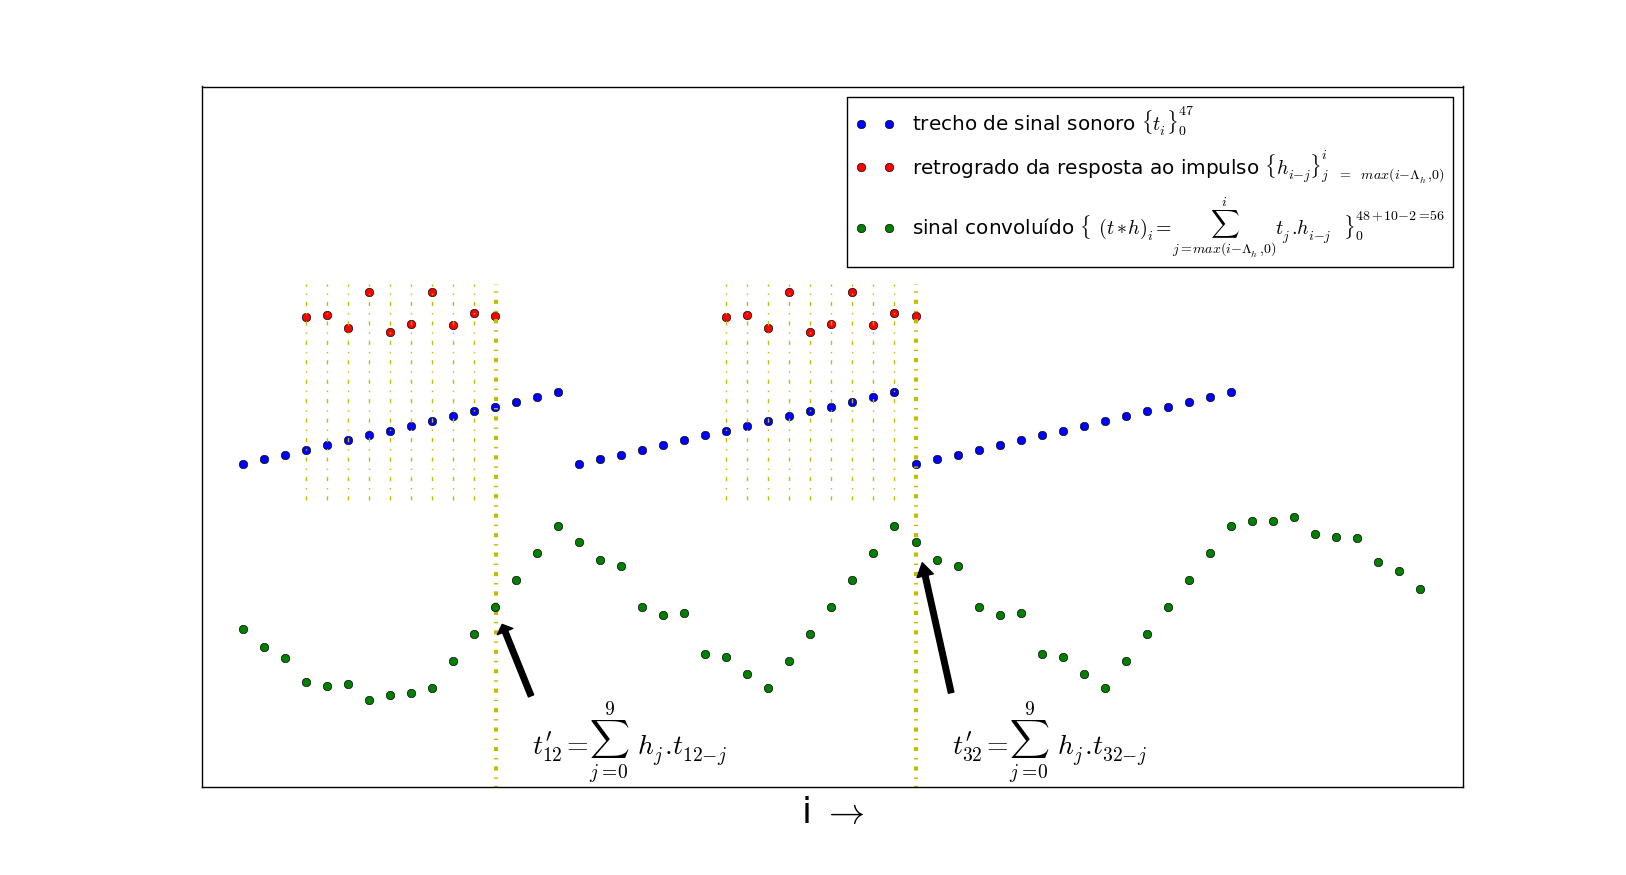
\includegraphics[width=\textwidth]{figuras/convolucao______}
        \label{fig:conv}
\end{figure}

Os filtros aplicados por convolução são conhecidos
pela sua sigla FIR (do inglês Finite Impulse Response)
e são caracterizados por possuirem uma representação amostral
finita no tempo. Esta representação amostral é chamada
de 'resposta ao impulso' $h_i$. Os filtros FIR são aplicados temporalmente ao som
digitalizado pela convolucão do som com a 
resposta ao impulso do filtro\footnote{Pode-se aplicar o filtro do domínio espectral através da multiplicação das transformadas de Fourier de ambos o som e a resposta ao impulso, e então realizada a transformada inversa de Fourier do espectro resultante~\cite{Openheim}.}. Para nossos fins, esta
convolução fica definida como:

\begin{equation}\label{eq:conv}
\begin{split}
\{t_i'\}_0^{\Lambda_t+\Lambda_h-2\; = \;\Lambda_{t\, '}-1} =\{(t*h)_i\}_0^{\Lambda_{t \, '}-1} & =\left \{ \sum_{j=0}^{min(\Lambda_h,i)}h_{j} . t_{i-j} \right \}_0^{\Lambda_{t\, '}-1} \\
    & =\left \{ \sum_{j=max(i-\Lambda_h,0)}^{i}t_j . h_{i-j} \right \}_0^{\Lambda_{t\, '}-1}
\end{split}
\end{equation}

Onde consideramos $t_i=0$ para as
amostras não definidas de antemão.
Ou seja, o som $\{t_i'\}$ resultante da convolução de $\{t_i\}$ com a resposta ao impulso $\{h_i\}$
tem cada i-ésima amostra $t_i$ substituída pela soma de suas últimas $\Lambda_h$ amostras $\{t_{i-j}\}_{j=0}^{\Lambda_h-1}$
multiplicadas uma a uma pela resposta ao impulso $\{h_i\}_0^{\Lambda_h-1}$ em si. Isso é facilmente
percebido pela visualização gráfica da convolução de sequências arbitrárias e dispomos
para este fim a figura \ref{fig:conv}. Observe que a resposta ao impulso $\{h_i\}$
é disposta na forma retrograda e que mostramos na figura os cálculos explícitos
das amostras $t_{12}'$ e $t_{32}'$ do sinal convoluído. O sinal resultante possui
sempre o tamanho $\Lambda_t+\Lambda_h -1=\Lambda_{t'}$.




Com este procedimento podemos aplicar reverberadores, equalizadores, delays
e vários outros tipos de filtros para fins de tratamento sonoro ou
efeitos musicais/artísticos.
 
Para a obtenção da resposta ao impulso, pode-se recorrer a medições
físicas ou à síntese direta do filtro. Para citar um exemplo
de medições diretas, uma resposta ao impulso para a aplicação
de reverberação pode resultar da gravação acústica do ambiente ao disparar
um estalo (cuja gravação se aproxima da resposta ao impulso diretamente) ou ao disparar uma
varredura de frequência (cuja gravação se aproxima da resposta em frequência).
Ambas resultam em respostas ao impulso
que, convoluídas com a sequência sonora, resultam na própria sequência
com uma reverberação que se assemelha à reverberação do ambiente 
em que ocorreu a medição~\cite{Cook}.

Como exemplo de resposta ao impulso sintetizada, pode-se
descrever um perfil espectral, realizar a transformada inversa
de fourier e convoluir o resultante com o som, realizando
uma filtragem cujo perfil é próximo ao especificado inicialmente. Note que este procedimento funciona particularmente bem se for grande o número de amostras utilizadas para especificar o perfil espectral do filtro\footnote{O que resulta em mais processamento computacional.}.

Outro exemplo simples e útil vem do deslocamento temporal causado pela convolução com o impulso deslocado. Assim, podemos aplicar de linhas de \emph{delays} através
da convolução do som com uma resposta ao impulso que possui um impulso
em cada reincidência do som na linha de delays intensionada.
Para ilustrar essa aplicação, dispomos a figura~\ref{fig:delays}
em que pode-se observar o deslocamento causado pela convolução
com o impulso. Dependendo da densidade dos impulsos, o resultado
é de caráter rítmico (20 impulsos por segundo ou menos) ou de amálgama
sonoro (20-40 impulsos por segundo ou mais). Neste último caso,
ocorrem processos tipicamente vinculados à síntese granular e às
equalizações.

\begin{figure}[h!]
    \centering
    \caption{Convolução com o impulso e linhas de delays}
        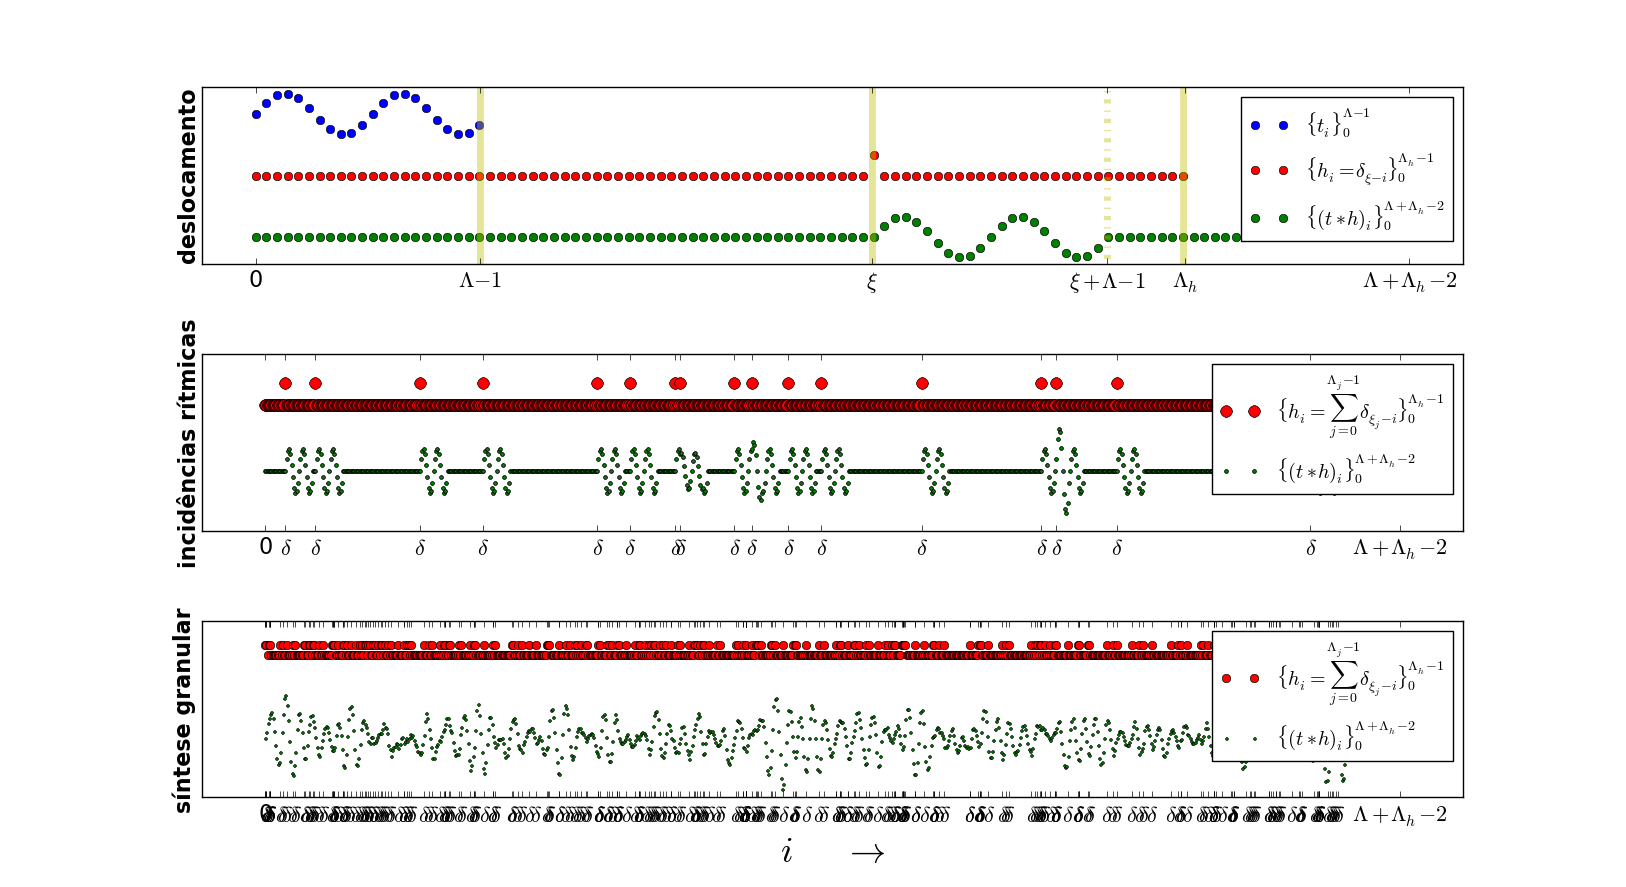
\includegraphics[width=\textwidth]{figuras/delays__}
        \label{fig:delays}
\end{figure}


\item Filtros de resposta ao impulso infinita (IIR)

Esta classe de filtros é
conhecida pela sigla IIR (do inglês Infinite Impulse Response)
e é caracterizada por possuir uma representação temporal
infinita, i.e. a resposta ao impulso não converge para zero. Sua aplicação é usualmente feita pela equação
a diferenças:

\begin{equation}
t_i' = \frac{1}{b_0}\left ( \sum_{j=0}^Ja_j . t_{i-j} - \sum_{k=1}^Kb_k . t_{i-k}' \right )
\end{equation}

com $b_0=1$ na grande maioria dos casos pois basta normalizarmos as variáveis
resultando em filtro idêntico: $a_j'=\frac{a_j}{b_0}$ e $b_k'=\frac{b_k}{b_0} \Rightarrow b_0' = 1$.

Apontamos filtros IIR bastante simples, úteis e usuais abaixo. Existem
diversos métodos e ferrametas para a elaboração de filtros IIR
e esta é uma seleção com fins didáticos e para consulta futura por
utilidade.
São filtros de primeira e segunda ordem bem comportados cujas
filtragens realizadas dispomos na figura~\ref{fig:iir}.

No caso dos filtros de ordem simples, a frequência de corte $f_c$ é onde 
o filtro realiza uma atenuação de $-3dB \approx 0.707 $ da amplitude original.
No caso dos filtros passa e rejeita banda, esta mesma atenuação é
resultado de duas especificações: $f_c$ (neste caso melhor compreendida como 'frequência central') e a largura de banda $bw$
pois em ambas as frequências $f_c \pm bw$ há uma atenuação de $\approx 0.707$ da amplitude original.

Observe que existe amplificação do som no caso dos filtros passa e rejeita banda quando a frequência
de corte é baixa e a largura de banda é grande o suficiente. Nos agudos, estes filtros apresentam
somente um desvio do perfil esperado, expandindo a envoltória um pouco mais do lado grave da banda em
evidência.

Para conseguir filtros cujas respostas em frequência possuem outras envoltórias (para o módulo),
o recurso mais simples a esta altura
é fazer cascata destes filtros aplicando-os sucessivamente.

Outra possibilidade é usar alguma receita de filtro
biquad\footnote{Abreviação
de 'biquadrado' pois sua função de transferência possue dois polos e dois zeros, i.e. sua
forma normal consiste em dois polinômios quadráticos formando uma fração
$\mathbb{H}(z)=\frac{a_0+a_1.z^{-1}+a_2.x^{-2}}{1+ b_1.z^{-1} +b_2 . z^{-2}}$.}
ou rotinas para cálculo de coeficientes
de filtros Chebichev\footnote{Filtros Butterworth e Elípticos podem
ser considerados como casos específicos dos Filtros do tipo Chebichev~\cite{Openheim,smith}.}.
Ambas as possibilidades são exploradas
por títulos em nossas referências, em especial recomendamos~\cite{JOSFM,smith} e a coleção de filtros da comunidade \emph{Music-DSP}, da Universiade de Columbia~\cite{music-dsp}.
Para uma exposição aprofundada do assunto, recomendamos~\cite{Openheim}.

\end{itemize}

\begin{enumerate}
\item Passa-baixas de polo simples com gráfico do canto superior esquerdo da figura~\ref{fig:iir}. A fórmula geral tem
por referência da frequência de corte $f_c \in (0,\frac{1}{2})$,
fração da frequência de amostragem $f_a$
em que há aproximadamente uma atenuação de $3dB$.
Calculamos os coeficientes do filtro IIR
$a_0$ e $b_1$ 
através da variável intermediária: $x \in [e^{-\pi},1]$:

\begin{figure}[h!]
    \centering
    \caption{Filtragens realizadas pelos filtros IIR das equações \ref{eq:passa-baixas}, \ref{eq:passa-altas}, \ref{eq:passa-banda} e \ref{eq:rejeita-banda}}
        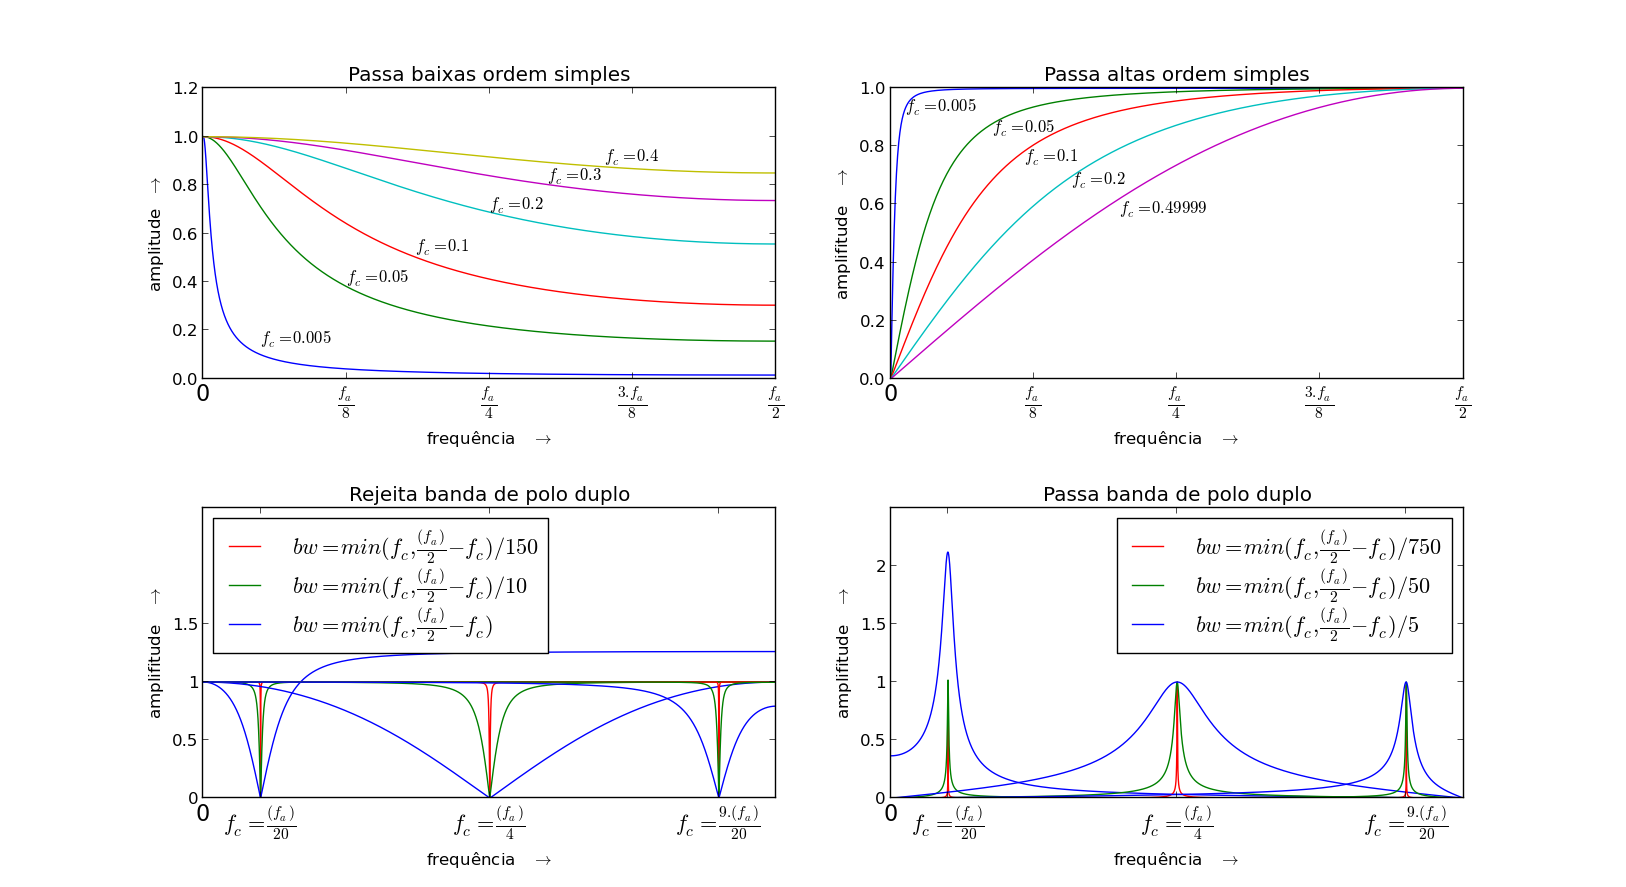
\includegraphics[width=\textwidth]{figuras/iir___}
        \label{fig:iir}
\end{figure}


\begin{equation}\label{eq:passa-baixas}
\begin{split}
x & =e^{-2\pi f_c} \\
a_0 & =  1-x \\
b_1 & =  x
\end{split}
\end{equation}

\item Passa-altas de polo simples com gráfico do canto superior direito da figura~\ref{fig:iir}. A fórmula geral,
com frequência de corte $f_c \in (0,\frac{1}{2})$, é calculada através da variável
intermediária $x \in [e^{-\pi},1]$:


\begin{equation}\label{eq:passa-altas}
\begin{split}
x & =e^{-2\pi f_c} \\
a_0 & =  \frac{x+1}{2} \\
a_1 & =  -\frac{x+1}{2} \\
b_1 & =  x
\end{split}
\end{equation}


%\item Passa-banda
%\item Rejeita-banda
\item Nó (\emph{notch filter}). Este filtro é parametrizado
pela frequência central\footnote{Não
confundir com a frequência de corte também notada aqui por $f_c$ nos filtros passa baixas e passa altas.} $f_c$
e a largura de banda $bw$
($f_c \pm bw$ resulta em 0.707 da amplitude, i.e. atenuação de $3dB$),
ambos dados como fracoes de $f_a$, portanto $f,\; bw \in (0,0.5)$.
Por conveniência definimos as variáveis auxiliares $K$ e $R$ como:

\begin{equation}
\begin{split}
R & = 1 - 3bw \\
K & = \frac{1-2R\cos(2\pi f_c) + R^2}{2 - 2 \cos (2 \pi f_c)}
\end{split}
\end{equation}

A partir das quais temos dois filtros. O filtro passa banda que dispomos no canto inferior esquerdo da figura~\ref{fig:iir}:

\begin{equation}\label{eq:passa-banda}
\begin{split}
a_0 & =  1 - K \\
a_1 & =  2(K-R)\cos (2\pi f_c) \\
a_2 & =  R^2-K \\
b_1 & =  2R \cos (2\pi f_c) \\
b_2 & =  -R^2
\end{split}
\end{equation}

e o filtro rejeita banda:

\begin{equation}\label{eq:rejeita-banda}
\begin{split}
a_0 & =  K \\
a_1 & =  -2K\cos (2\pi f_c) \\
a_2 & =  K \\
b_1 & =  2R \cos (2\pi f_c) \\
b_2 & =  -R^2
\end{split}
\end{equation}

disposto na parte inferior esquerda da figura~\ref{fig:iir}.

%\item Biquad: pela especificação de uma frequência central, da qualidade
%e da intensidade do filtro, este filtro é simples e usual para áudio,
%permitindo ajustes mais finos. Diversas receitas podem ser encontradas
%na literatura, recomendamos especialmente as diferentes especificações
%em ~\ref{musicDSP} e ~\ref{dspguide}.

\end{enumerate}

\subsection{Ruídos}
De forma geral, os sons sem altura definida 
são chamados ruídos~\cite{Lacerda}.
Estes sons estão presentes como constituintes importantes dos sons musicais de altura definida,
como os ruídos presentes nas notas do piano, do violino, etc. Além disso, os instrumentos
de percussão, em grande parte, não possuem altura definida e seus sons
são muitas vezes compreendidos como ruídos~\cite{Roederer}. Na música eletrônica (incluindo
a eletroacústica e gêneros de pista de dança), os ruídos possuem usos amplos, diversificados e comumente
idiomáticos~\cite{Cook}.

A ausência de uma altura definida é fruto da ausência de uma organização harmônica perceptível nas componentes senoidais que formam o som. Assim, pode-se inferir
as incontáveis possibilidades de gerar ruídos. A mais imediata é a utilização
de valores aleatórios para a geração da sequência sonora $T_i$. Este
é um método atraente, visto a disponibilidade
das consagradas distribuições de probabilidade em diversas linguagens de programação,
mas os resultados não são tão úteis, tendendo geralmente ao ruído branco
e com difíceis previsões do espectro resultante~\cite{Cook}.

Outra possibilidade é a geração de ruído através do espectro desejado. A partir
dele, executamos a transformada inversa de Fourier. Neste caso, é importante
que realizemos a distribuição espectral com cuidado pois queremos um perfil
do módulo do espectro e a fase é aleatória\footnote{Caso utilizemos a mesma fase
(ou fases com forte correlação) para
as componentes envolvidas, o som sintetizado possuirá energia bastante concentrada
em alguns trechos.}. Veja a figura~\ref{fig:ruidos} e o código Python que a gerou para uma implementação.


\begin{figure}[htpq!]
    \centering
    \caption{Ruídos coloridos realizados através das equações~\ref{eq:branco}, \ref{eq:rosa}, \ref{eq:marrom}, \ref{eq:azul}, \ref{eq:violeta}: espectros e ondas sonoras resultantes}
        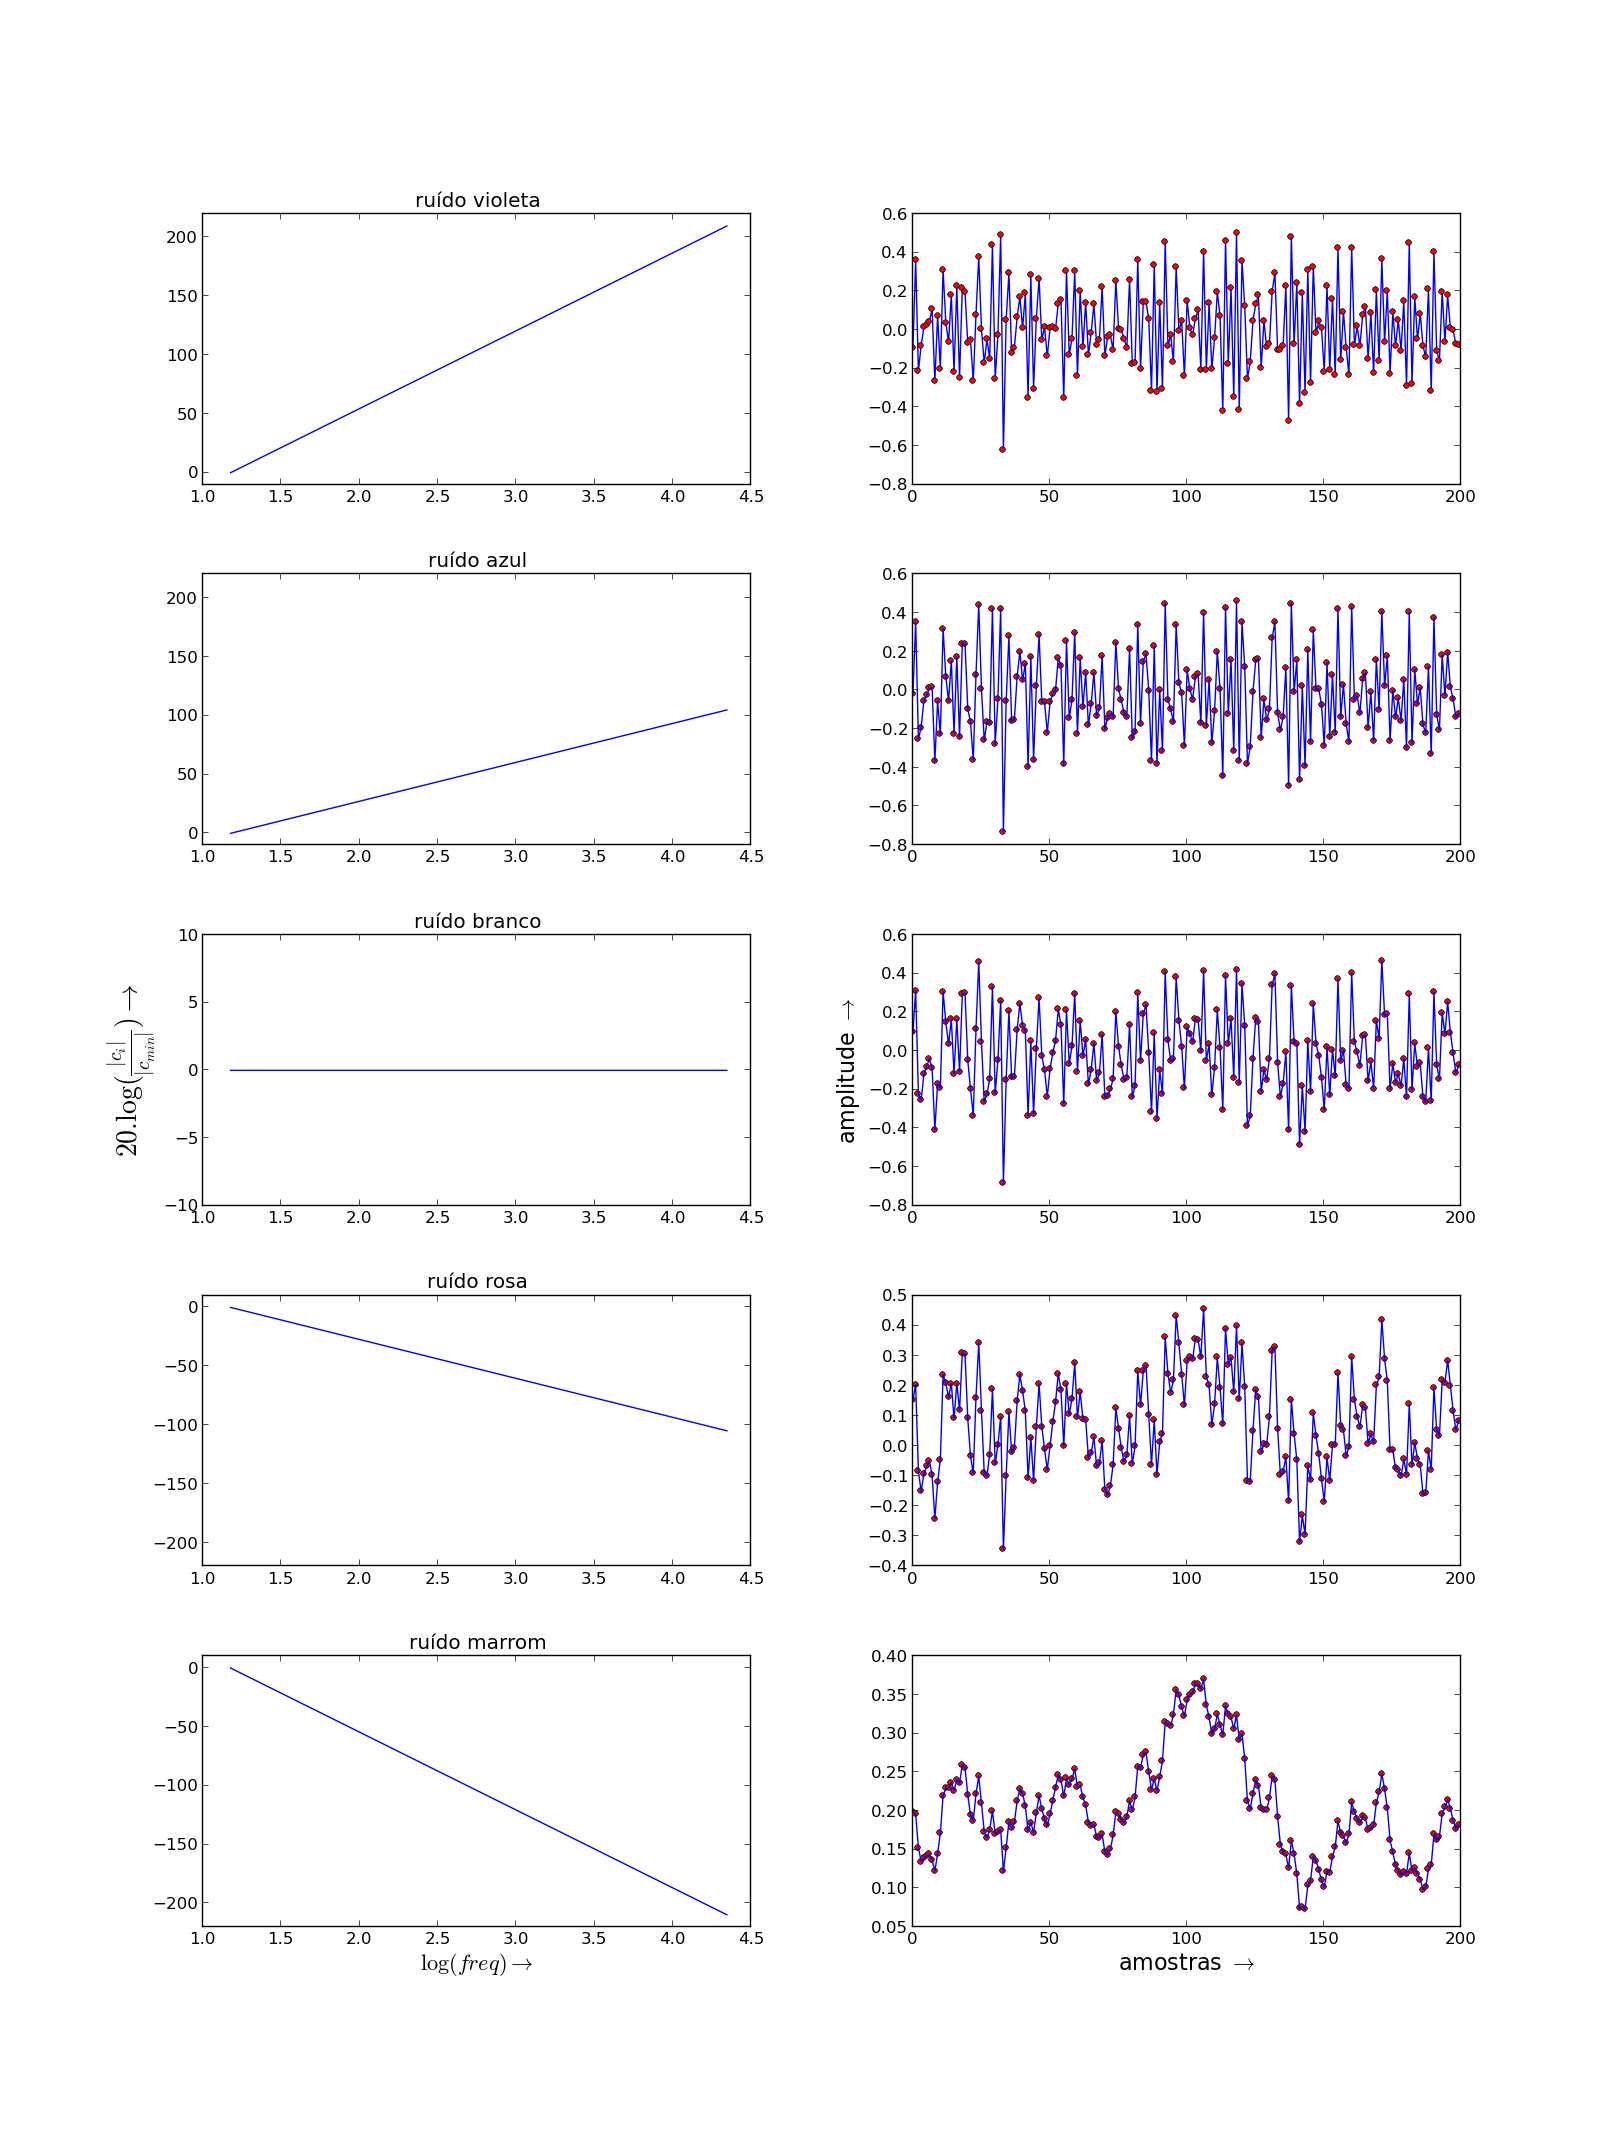
\includegraphics[width=\textwidth]{figuras/ruidos___}
        \label{fig:ruidos}
\end{figure}


Abaixo elencamos alguns ruídos de espectros estáticos. São chamados \emph{coloridos} por terem sido associados a cores. 

\begin{itemize}

\item O ruído branco deve seu nome por possuir energia distribuida
igualmente por todas as frequências. Podemos obter a realização
do ruído branco com a transformada inversa dos seguintes coeficientes:


\begin{equation}\label{eq:branco}
\begin{split}
c_0 & =0 \quad \text{pois não queremos bias} \\
c_i & =e^{j.x}\;,\;\; j^2=-1 \;, \;\; x \; \text{randômico} \; \in \; [0,2\pi]\;,\;\; i \; \in \; \left[1, \, \frac{\Lambda}{2}-1\right] \\
c_{\Lambda/2} & = 1 \quad\quad \text{(se $\Lambda$ par)}\\ 
c_i & = c_{\Lambda - i}^*\;,\;\; \text{para}\;  i \; > \;  \frac{\Lambda}{2}
\end{split}
\end{equation}

O valor de $c_i$ calculado pela exponencial é apenas um artifício para resultar em módulo unitário e fase aleatória.
Já $c_{\Lambda/2}$ é sempre puramente real (como vimos na sessão anterior).

\item O ruído rosa possui uma queda de $3dB$ por oitava. Este ruído é muito usual no teste de equipamentos e montagens de aparelhos além de presença destacada na natureza~\cite{Roederer}. 

\begin{equation}\label{eq:rosa}
\begin{split}
f_{\text{min}} & \approx 15 Hz \\
f_i & = i \frac{f_a}{\Lambda} \;, \;\; \quad i \;\leq\; \frac{\Lambda}{2},\;\; i\;\in\;\mathbb{N}  \\
\alpha_i & = (10^{-\frac{3}{20}})^{\log _2 \left ( \frac{f_i}{f_{\text{min}}} \right )}  \\
c_i & =0\;,\;\; \forall \; i \; : f_i<f_{\text{min}} \\
c_i & =e^{j.x} . \alpha_i\;,\;\; j^2=-1 \;, \;\;\  x \;\; \text{randômico} \; \in \; [0,2\pi]\;,\;\; \forall \; i \; : f_{\text{min}} \le f_i < f_{\lceil \Lambda/2-1 \rceil}  \\
c_{\Lambda/2} & = \alpha_{\Lambda/2} \quad\quad \text{(se $\Lambda$ par)}\\ 
c_i & = c_{\Lambda - i}^*\;,\;\; \text{para}\;  i \; > \;  \Lambda/2
\end{split}
\end{equation}

A frequência mínima $f_{\text{min}}$ pode ser escolhida com base no limite da audição, pois não escutamos como altura uma componente sonora cuja frequência esteja abaixo de $\approx\; 20Hz$.

O resto dos ruídos podem ser feitos com base neste procedimento descrito para 
o ruído rosa. Basta que modifiquemos alguns detalhes. Em especial a equação que define $\alpha_i$.

\item O ruído marrom deve seu nome ao Robert Brown, que descreveu o movimento browniano.
Embora esta origem seja um tanto díspar do que poderíamos considerar motivo para uma associação com a cor marrom, o ruído sonoro ficou consagrado com este nome. De qualquer forma, é bastante comum declarar satisfatória a associação do ruído com a cor marrom, dados os ruídos branco e rosa mais estridentes e relacionados a cores mais intensas~\cite{marrom}.

O que caracteriza este ruído é a queda de $6dB$ por oitava. Desta forma, basta modificarmos a equação de $\alpha_i$ 
no conjunto \ref{eq:rosa} para:

\begin{equation}\label{eq:marrom}
\alpha_i=(10^{-\frac{6}{20}})^{\log _2 \left( \frac{f_i}{f_{\text{min}}} \right )}
\end{equation}

\item Ruído azul é aquele em que há um ganho de $3dB$ por oitava em uma banda limitada. Para
a síntese deste ruído, basta estipularmos a frequência mínima $f_{\text{min}}$ e a frequência
máxima $f_{\text{máx}}$. Assim, também com base no conjunto de equações \ref{eq:rosa}, 
basta atentarmos para as sequintes identidades:

\begin{equation}\label{eq:azul}
\begin{split}
\alpha_i & = (10^{\frac{3}{20}})^{\log _2 \left ( \frac{f_i}{f_{\text{min}}} \right )} \\
c_i & =0\;,\;\; \forall \; i \; : f_i<f_{\text{min}} \;\; \text{ou} \;\; f_i>f_{\text{máx}} \\
\end{split}
\end{equation}

\item O ruído violeta é similar ao ruído azul, mas o ganho é de $6dB$ por oitava:

\begin{equation}\label{eq:violeta}
\alpha_i = (10^{\frac{6}{20}})^{\log _2 \left ( \frac{f_i}{f_{\text{min}}} \right )} \;\;, \quad f_{\text{min}} \approx 15 Hz \\
\end{equation}

\item O ruído preto possui perdas maiores que $6dB$ por oitava, assim:

\begin{equation}\label{eq:preto}
\alpha_i=(10^{-\frac{\beta}{20}})^{\log _2 \left( \frac{f_i}{f_{\text{min}}} \right )}\;\;, \quad \beta > 6
\end{equation}



\item Um pouco diferente dos exemplos acima é o ruído cinza, definido como
um ruído branco sujeito a uma das curvas iso-audíveis. Como estas curvas são resultados
experimentais, precisamos neste caso da curva para a realização dos fatores multiplicativos
$\alpha_i$.

\end{itemize}

Com base nestes ruídos expostos podemos prever a infinidade de ruídos utilizados. Importante
neste momento é entender que foram expostos somente ruídos com espectro estático. Existem classificações
de ruídos com variações do espectro no decorrer do tempo. Existem também ruídos que
são fundamentalmente transientes, como os clicks e os chirps. O primeiro é modelado
facilmente por um impulso relativamente isolado, enquanto o segundo é uma varredura rápida de 
alguma banda de frequência~\cite{Cook}.

Os ruídos das equações \ref{eq:branco}, \ref{eq:rosa}, \ref{eq:marrom},
\ref{eq:azul}, \ref{eq:violeta} estão na figura \ref{fig:ruidos}. Vale notar
que os espectros foram feitos com a mesma fase nos coeficientes, de forma que
pode-se observar a contribuição dos harmônicos agudos no traçado geral dado
pelas frequências graves e muito explícito no ruído marrom.


\subsection{Usos musicais parte 1: trêmolo e vibrato, AM e FM}

Enquanto o vibrato é uma variação periódica de altura (frequência),
o tremolo é uma variação periódica de volume (intensidade).\footnote{Alguns instrumentos e contextos musicais usam nomenclaturas diferentes. Por exemplo, no piano, o chamado trêmolo é um vibrato e um tremolo segundo a classificação aqui utilizada. As definições presentes neste trabalho tem por base uma literatura mais abrangente do que a utilizada para um único instrumento, prática ou tradição musical e comum em contextos de teoria musical e musica eletrônica~\cite{Lacerda,Harmonia}.}

Iniciemos pelo vibrato. Para realizarmos o caso mais geral, façamos uma sequência $t_i'$
de frequência $f'$ com o auxílio
de uma segunda tabela $\widetilde{M}_i$ de tamanho $\widetilde{\Lambda}_M$ que apresente também
um período de onda que oscila entre $[-1,1]$. Descrevemos uma sequência sonora $t_i^{vbr(f',\,\nu)}$ com
um vibrato de frequência $f'$ e profundidade  $\mu$ (quantos herz é a oscilação no pico superior)
ou $\nu$ (amplitude do vibrato em semitons) da seguinte forma:


\begin{equation}\label{vbrGamma}
\gamma_i'=\left \lfloor i f' \frac{\widetilde{\Lambda}_M}{f_a} \right \rfloor
\end{equation}

\begin{equation}\label{vbrAux}
t_i'=\widetilde{m}_{\gamma_i' \;\% \widetilde{\Lambda}_M}
\end{equation}

\begin{equation}\label{vbrF}
f_i=f \left ( \frac{f + \mu }{f} \right )^{t_i'}=f . 2^{t_i'\frac{\nu}{12}}
\end{equation}

\begin{equation}\label{vbrGamma2}
\Delta_{\gamma_i}=f_i\frac{\widetilde{\Lambda}}{f_a} \quad \Rightarrow \quad \gamma_i = \left \lfloor \sum_{j=0}^{i} f_j \frac{\widetilde{\Lambda}}{f_a} \right \rfloor = \left \lfloor \sum_{j=0}^{i} \frac{\widetilde{\Lambda}}{f_a}f \left ( \frac{f + \mu }{f} \right )^{t_j'}  \right \rfloor= \left \lfloor \sum_{j=0}^{i} \frac{\widetilde{\Lambda}}{f_a}f . 2^{t_j'\frac{\nu}{12}}  \right \rfloor
\end{equation}

\begin{equation}\label{vbrT}
T_i^{f, vbr(f',\,\nu)}=\{ t_i^{f,vbr(f',\,\nu)} \}_0^{\Lambda-1}=\{ \widetilde{l}_{\gamma_i \%\; \widetilde{\Lambda} } \}_0^{\Lambda-1}
\end{equation}


\begin{figure}[h!]
    \centering
    \caption{Espectrograma de um som com vibrato senoidal de $3Hz$ e profundidade de uma oitava em uma dente de serra de $1000Hz$ (considerada $f_a=44.1kHz$)}
        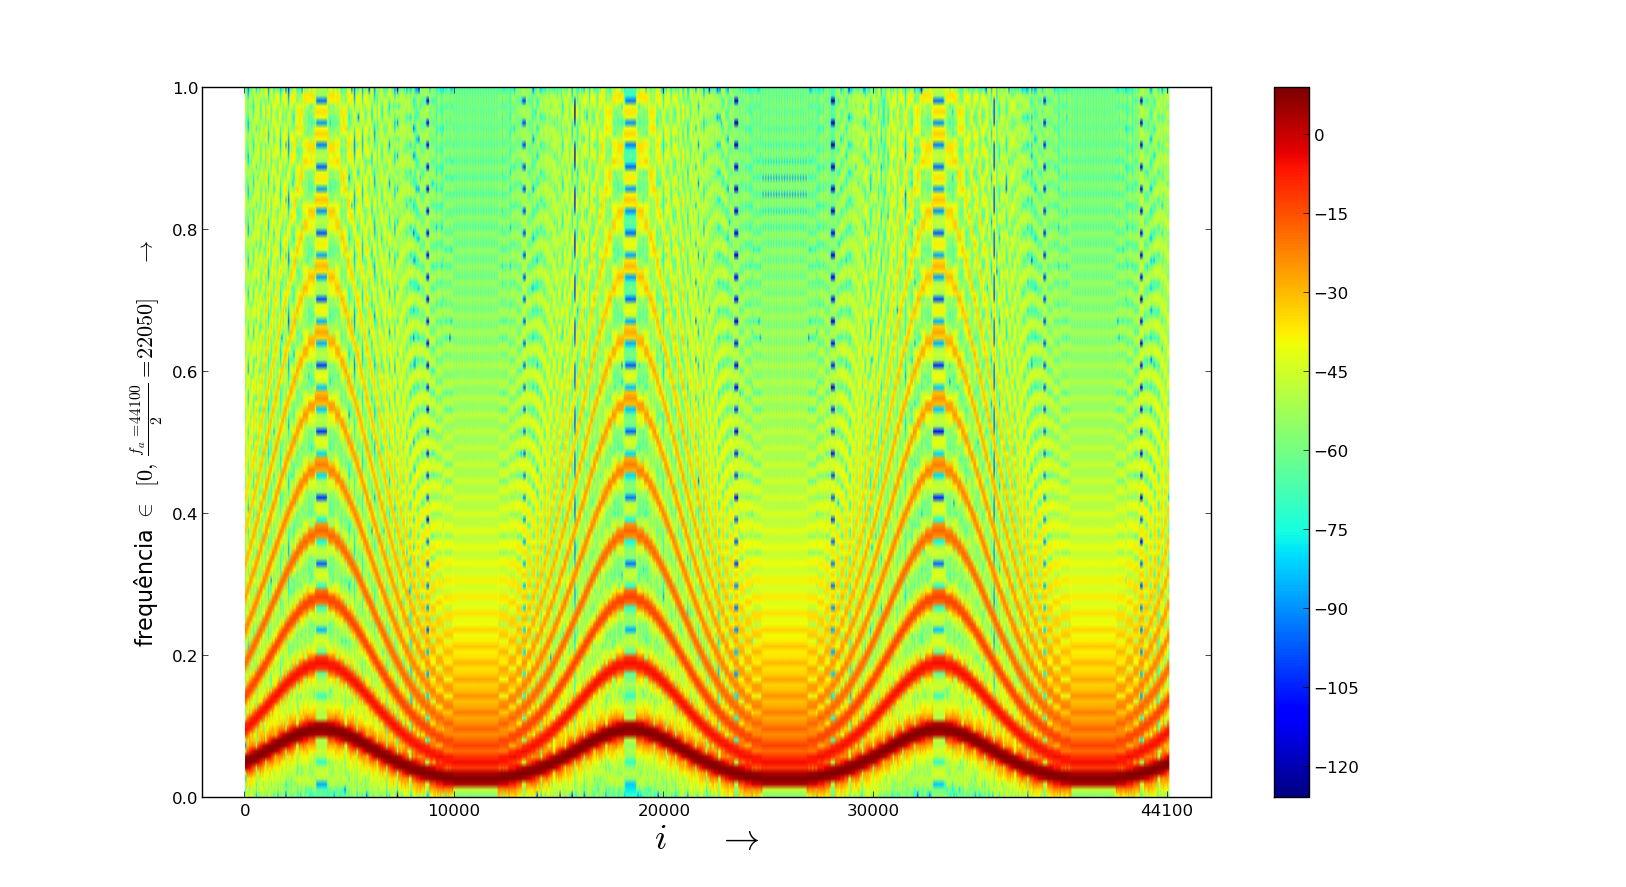
\includegraphics[width=\textwidth]{figuras/vibrato___}
        \label{fig:vibrato}
\end{figure}

Para a correta realização do vibrato, é importante atenção para as duas tabelas e sequências.
A tabela $\widetilde{M}_i$ de tamanho $\widetilde{\Lambda}_M$ e a sequência de índices $\gamma_i'$ formam a sequência $t_i'$
 que é o padrão da oscilação da frequência enquanto
a tabela $\widetilde{L}_i$ de tamanho $\widetilde{\Lambda}$ e a sequência de índices $\gamma_i$ formam $t_i$ que é o som em si.
As variáveis $\mu$ e $\nu$ quantificam a intensidade do vibrato: $\mu$ é uma medida direta da quantidade
de Herz envolvidos no limite superior da oscilação e $\nu$ é a medida direta de semitons envolvidos na oscilação ($2\nu$ é o número de semitons entre os picos superioes e inferiores de oscilação da frequência do som $\{t_i\}$ causada pelo vibrato).
Note que $\nu=\log_{2}\frac{f+\mu}{f} $ é conveniente neste caso pois o aumento máximo de frequência
não equivale à diminuição máxima, mas a variação de semitons se mantém.

A Figura \ref{fig:vibrato} é o espectrograma de um vibrato artificial de uma nota em
$1000Hz$ (entre um si e um dó) e cujo desvio da frequência atinge uma oitava
para cima e para baixo. Note o padrão senoidal do vibrato e as compontentes harmônicas
da dente de serra. Qualquer forma de onda pode
ser utilizada para gerar o som e o padrão de oscilação do vibrato, o que é tão crucial para os usos musicais quanto a
frequência de oscilação e o desvio de altura envolvido\footnote{O desvio de altura
é chamado profundidade do vibrato e é geralmetne dado por conveniência em semitons ou cents.}. Estas qualidades não são praticáveis em instrumentos musicais tradicionais, introduzindo novidade nas possibilidades artísticas.

O caso do tremolo é semelhante e $f'$, $\gamma_i'$ e $t_i'$ permanecem os mesmos. Calculamos
a sequência de amplitudes a serem multiplicadas pela sequência original $t_i$ da
sequinte forma:

\begin{equation}\label{trA}
a_i=10^{\frac{V_{dB}}{20}t_i' } = a_{\text{máx}}^{t_i'}
\end{equation}

\begin{equation}\label{trT}
T_i^{tr(f')}=\{ t_i^{tr(f')} \}_0^{\Lambda-1}=\{ t_i . a_i \}_0^{\Lambda-1}=\{t_i .10^{t_i' \frac{V_{dB}}{20}}    \}_0^{\Lambda-1}=\{t_i . a_{\text{máx}}^{t_i'}\}_0^{\Lambda-1}
\end{equation}

Onde $V_{dB}$ é a profundidade da oscilação em decibels do trêmolo e $a_{\text{máx}}=10^{\frac{V_{dB}}{20}}$
 é o ganho máximo de amplitude envolvido.
A medição em decibels é bastante pertinente pois o aumento máximo de amplitude
não equivale à diminuição máxima relacionada, enquanto a diferença em decibels se mantém.

A figura~\ref{fig:tremolo} mostra a amplitude das sequências $\{a_i\}_0^{\Lambda-1}$ e $\{t_i'\}_0^{\Lambda-1}$
para três oscilações de um trêmolo com forma da dente de serra. A curvatura é devido à progressão logarítmica de
intensidade. A frequência do trêmolo é de $1,5Hz$ pois $f_a=44,1kHz \; \Rightarrow \; \text{duração} = \frac{i_{\text{máx}}=82000}{f_a}= 2s \; \Rightarrow \; \frac{3\text{oscilações}}{2s}=1,5$ oscilações por segundo ($Hz$). 

A montagem musical \emph{Vibra e treme} explora estes recursos dos tremolos e vibratos
com frequências $f'$
e profundidades ($\nu$ e $V_{dB}$) diferentes. Usados em associação e isoladamente os tremolos e vibratos e com variações progressivas dos parâmetros\footnote{Vale lembrar que os tremolos e vibratos ocorrem muitas vezes juntos em instrumentos tradicionais e na voz.}. A peça desenvolve também uma comparação entre os vibratos e tremolos em escala logarítmica e em escala linear para uma apreciação qualitativa.


\begin{figure}[h!]
    \centering
    \caption{Tremolo de profundidade $V_{dB}=12dB$ com padrão oscilatório de uma dente de serra em $f'=1.5Hz$ em uma senoide de $f=40Hz$ (considerada taxa de amostragem $f_a=44,1kHz$)}
        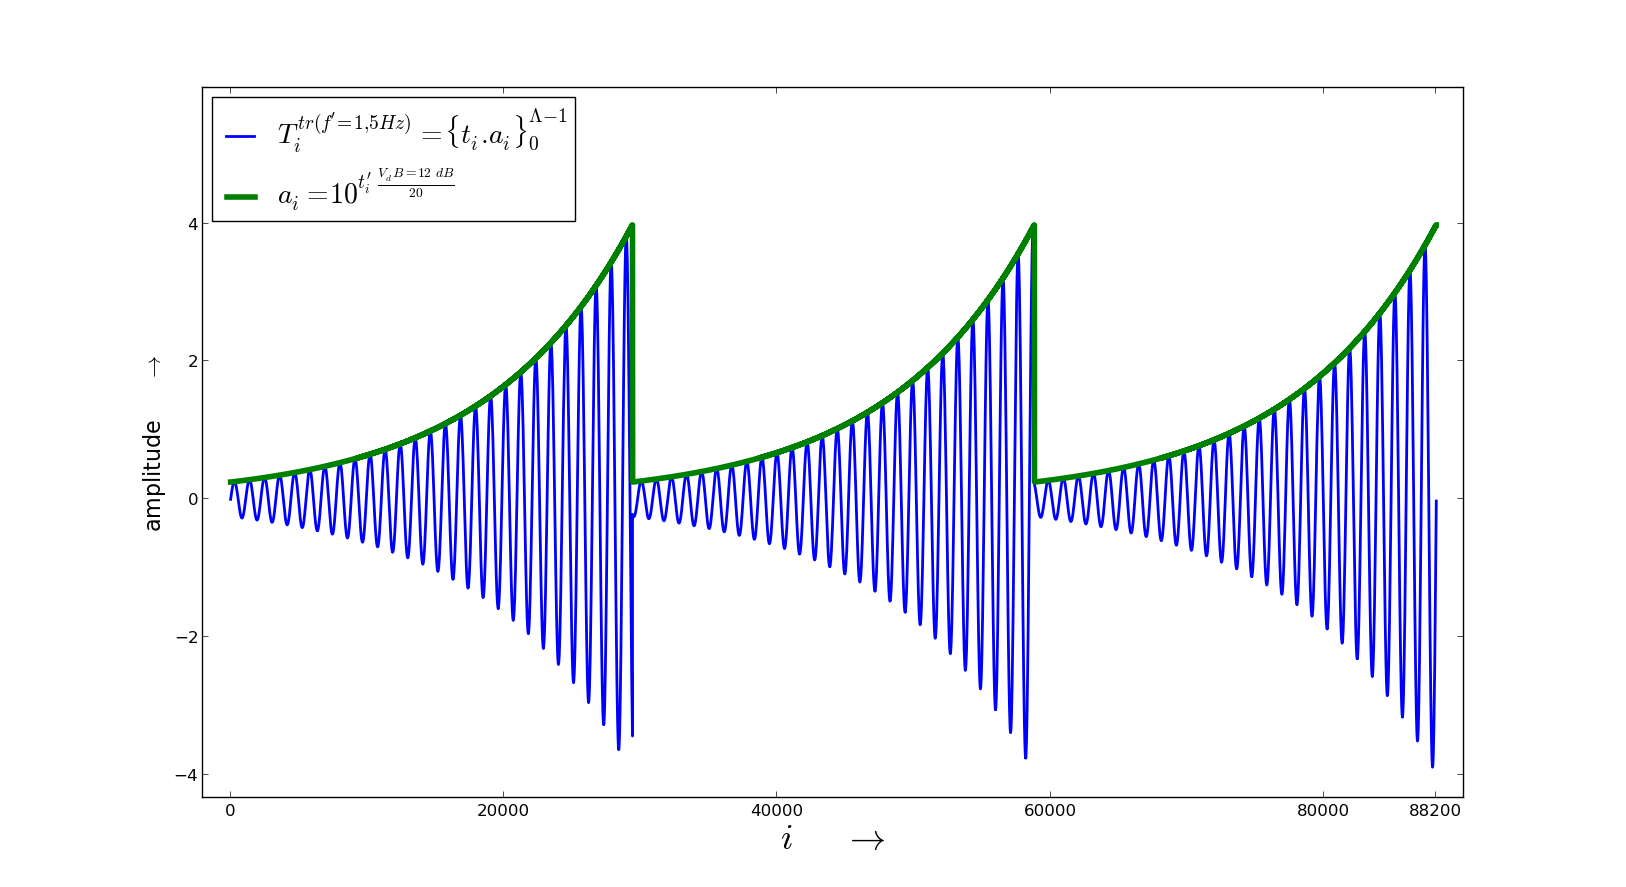
\includegraphics[width=\textwidth]{figuras/tremolo}
        \label{fig:tremolo}
\end{figure}

Algo interessante ocorre se aumentarmos progressivamente $f'$.
Primeiramente a aproximação do limiar de frequência
para audição do fenômeno sonoro como
altura ($\approx 20Hz$) gera rugosidades para
ambos tremolos e vibratos. Estas rugosidades são muito apreciadas
tanto na tradição erudita quanto na música eletrônica atual, especialmente no \emph{Dubstep}~\cite{DubRugoso}.
A rugosidade também é gerada através de conteúdos espectrais que geram batimentos~\cite{Porres}.  A sequência \emph{Rugosidades}
explora este limiar com concomitâncias de tremolos e vibratos na mesma
voz, com intensidades e formas de onda diferentes.

Se continuarmos aumentando a frequência, deixamos de ouvir estas oscilações
como eventos identificáveis. Neste caso, as oscilações se apresentam na forma de espectro
audível como altura, $f'$, $\mu$ e a forma de onda realizam alterações espectrais no som
original $T_i$ de formas diferentes para os tremolos e para os vibratos, são as 
chamadas sínteses AM (\emph{Amplitude Modulation}) e FM (\emph{Frequency Modulation}), respectivamente.
Estas são técnicas muito poderosas e conhecidas, com clássicas aplicações em sintetizadores
históricos como o \emph{Yamaha DX7} e com aplicações fora da música, como em telecomunicações para transmissão de informação via ondas eletromagnéticas (ex. radios AM e FM).

Para fins musicais e em resumo, podemos entender a síntese FM através do caso entre senoides
e decompor os sinais em seus espectros de Fourier (i.e. senoidais) para casos mais complexos.
Assim, a síntese FM realizada com um 'vibrato' senoidal de frequência $f'$ e profundidade $\mu$ em um som também senoidal $T_i$ de frequência $f$
e duração $\Delta$ segundos (assumimos $\Lambda = \lfloor \Delta . f_a \rfloor $ amostras)
gera bandas centradas em $f$ e distantes $f'$ entre si:

\begin{equation}\label{eq:fmEsp}
\begin{split}
\{t_i'\}_0^{\Lambda -1} & = \left \{ \cos \left [f . 2 \pi \frac{i}{f_a-1} + \mu . sen \left ( f' . 2 \pi \frac{i}{ f_a -1 } \right ) \right ] \right \}_0^{\Lambda-1}  = \\
 & = \left \{ \sum_{k=-\infty}^{+\infty} J_k(\mu) \cos \left [ f . 2 \pi \frac{i}{f_a-1} + k . f' . 2 \pi \frac{i}{f_a-1} \right ]  \right \}_0^{\Lambda-1} = \\
 & = \left \{ \sum_{k=-\infty}^{+\infty} J_k(\mu) \cos \left [ (f+k.f') . 2 \pi \frac{i}{f_a-1} \right ]  \right \}_0^{\Lambda-1}
\end{split}
\end{equation}

onde 
\begin{equation}
J_k(\mu) = \frac{2}{\pi} \int_0^{\frac{\pi}{2}}\left [ cos \left (\overline{k}\;\frac{\pi}{2} + \mu . \sin w \right ) . cos \left ( \overline{k}\;\frac{\pi}{2} + k . w \right ) \right ] dw \quad , \quad \overline{k} = k \% 2 \;\;,\;\; k \in \mathbb{N}
\end{equation}
é a função de Bessel~\cite{BesselCCRMA,JOSFM} que, na FM, como podemos notar, especifica a amplitude de cada componente. Note que, nestas equações, a variação de frequência introduzida por $\{t_i'\}$ não respeita a progressão geométrica de frequência que acompanha a percepção de altura. Caso utilizemos as equações~\ref{vbrF} teríamos uma distribuição diferente dos harmônicos. Para este fim, dispomos o APÊNDICE~\ref{cap:fmam} onde calculamos o conteúdo espectral da síntese FM feita com oscilações na escala logarítmica. De fato, como pode-se notar nos cálculos, o comportamento simples que torna a FM atraente é obtido somente com as variações lineares utilizadas em~\ref{eq:fmEsp}.

O caso da modulação de amplitude (AM) é mais simples:

\begin{equation}\label{eq:am}
\begin{split}
\{t_i'\}_0^{\Lambda-1} & =\{(1+a_i) . t_i\}_0^{\Lambda-1}= \left \{ \left [ 1+M.\sin \left ( f'.2\pi\frac{i}{f_a -1} \right ) \right] . P .\sin \left ( f.2\pi\frac{i}{f_a -1} \right ) \right \}_0^{\Lambda-1} = \\
& = P.\sin \left( f.2\pi\frac{i}{f_a -1}  \right ) + \frac{P.M}{2} \left [ \sin \left( (f-f').2\pi\frac{i}{f_a -1}  \right ) + \sin \left( (f+f').2\pi\frac{i}{f_a -1}  \right ) \right ]
\end{split}
\end{equation}

Ou seja, o som resultante é o som original
e a reprodução de seu conteúdo espectral acima e abaixo da frequência
original, distantes $f'$ de $f$. Observe que utilizamos novamente a variação na escala linear de amplitude. Dispomos no APÊNDICE~\ref{cap:fmam} uma exposição do espectro da AM se realizada a oscilação na escala logarítmica de amplitude, que também perde o comportamento simples.

A realização da FM e AM através de LUTs é consideravelmente simples.
A frequência $f$ a ser modulada, chamada portadora, é modulada pela $f'$, chamada moduladora. No jargão de FM e AM, $\mu$ e $\alpha=10^{\frac{V_{dB}}{20}}$ são chamados índices de modulação. Assim, temos
para o padrão de vibração da moduladora $\{t_i'\}$ as mesmas equações utilizadas para os tremolos e vibratos:

\begin{equation}\label{fmGamma}
\gamma_i'=\left \lfloor i f' \frac{\widetilde{\Lambda}_M}{f_a} \right \rfloor
\end{equation}

\begin{equation}\label{fmAux}
t_i'=\widetilde{m}_{\gamma_i' \;\% \widetilde{\Lambda}_M}
\end{equation}

Para aplicação da moduladora $\{t_i'\}$ na portadora $\{t_i\}$,
temos, para a FM:

\begin{equation}\label{fmF}
f_i=f + \mu . t_i'
\end{equation}

\begin{equation}\label{fmGamma}
\Delta_{\gamma_i}=f_i\frac{\widetilde{\Lambda}}{f_a} \quad \Rightarrow \quad \gamma_i = \left \lfloor \sum_{j=0}^{i} f_j \frac{\widetilde{\Lambda}}{f_a} \right \rfloor = \left \lfloor \sum_{j=0}^{i} \frac{\widetilde{\Lambda}}{f_a}(f+\mu . t_j') \right\rfloor
\end{equation}

\begin{equation}\label{fmT}
T_i^{f,\, FM(f',\,\mu)}=\left\{ t_i^{f,\,FM(f',\,\mu)} \right\}_0^{\Lambda-1}=\left\{\,\widetilde{l}_{\gamma_i \%\; \widetilde{\Lambda} } \,\right\}_0^{\Lambda-1}
\end{equation}

Onde $\widetilde{l}$ é um período da forma de onda de comprimento $\widetilde{\Lambda}$ da portadora.

Para realizar a AM, basta modular $\{t_i\}$ com $\{t_i'\}$ através das equações (lembrando que $\alpha=10^{\frac{V_{dB}}{20}}$):

\begin{equation}\label{amA}
a_i=1 + \alpha . t_i'
\end{equation}

\begin{equation}\label{trT}
T_i^{f,\,AM(f',\,\alpha)}=\left\{ t_i^{f,\,AM(f',\,\alpha)} \right\}_0^{\Lambda-1}=\{ t_i . a_i \}_0^{\Lambda-1}=\{t_i . (1 + \alpha . t_i')    \}_0^{\Lambda-1}
\end{equation}



\subsection{Usos musicais parte 2}
A este ponto as possibilidades musicais explodiram. Possuímos unidades
musicais com características próprias de altura (dada pela frequência),
tímbre (dado pela forma de onda),
volume (dado pela intensidade) e duração (dada pelo número de amostras).
Em uma nota, estas características podem ser consideradas
de forma absoluta ou tratadas ao longo de sua duração,
com a única excessão da duração em si.

Desta forma, os usos musicais que apresentamos é uma coleção de possibilidades
com o objetivo de exemplificar manipulações sonoras que resultem algo
musical, por razões variadas e aprofundadas na próxima sessão.

Uma primeira possibilidade interessante é o estabelecimento de vínculos
entre os parâmetros do trêmolo e do vibrato e algum parâmetro da nota básica,
digamos a frequência. Assim, podemos estabelecer que quanto mais aguda é a nota,
mais alta é a frequência do vibrato e do trêmolo mas menor a sua profundidade.
Desta forma, tomando por base as equações \ref{vbrGamma}, \ref{vbrF} e \ref{trA}
podemos escrever:

\begin{equation}
\begin{split}
f^{vbr} = f^{tr} & = func_a(f) \\
\nu & = func_b(f) \\
V_{dB} & = func_c(f)
\end{split}
\end{equation}

Com $f^{vbr}$ e $f^{tr}$ sendo $f'$ nas equações de referência, ou seja, a frequência
de oscilação do vibrato e do tremolo utilizada na equação~\ref{vbrGamma}. Já $\nu$ e $V_{dB}$ são as profundidades
do vibrato e do tremolo, respectivamente. As funções $func_a$,
$func_b$ e $func_c$ são arbitrárias e dependentes das intensões musicais. A montagem musical 
\emph{Tremolos, vibratos e a frequência} explora
recursos como este e variações da forma de onda da oscilação com vínculos, de modo a formar um \emph{idioma musical}\footnote{Veja na próxima sessão.}.


Com relação à convolução, podemos estabelecer uma duração como pulso musical - a exemplo de um pulso BPM - 
e distribuir impulsos no decorrer deste pulso, de forma a estabelecer métricas e rítmos\footnote{Lembrando
que a convolução com o impulso resulta no som deslocado ao instante de ocorrência do impulso.}.
Por exemplo, se escolhemos 2 impulsos igualmente espaçados, estaremos fazendo uma
divisão binária básica do pulso. Se escolhemos dois sinais, um com 2 pulsos e outro com 3 pulsos,
ambos com os impulsos igualmente espaçados na duração do pulso, resultamos na manutenção
do pulso, com uma marcação rítmica usada tanto em divisões binárias quanto ternárias em diversos
estilos de música étnica e tradicional~\cite{Gramani}. 
Os próprios valores absolutos destes impulsos resultam em proporções entre as amplitudes dos sinais
convoluídos.
Exploramos este recurso da métrica
estabelecida pela convolução com impulsos na sequência musical \emph{trenzinho de caipiras impulsivos}. Os recursos explorados incluem a criação de amálgamas sonoros provenientes da síntese granular e esta montagem é já uma ponte para a próxima sessão. Veja especialmente a figura~\ref{fig:pulsoSubAgl}.

Já com os filtros as possibilidades explodem ainda mais vertiginosamente. Pode-se convoluir um sinal para reverberá-lo, para
remover algum ruído, para gerar distorções ou para tratamento com intuito estético mesmo (soa melhor por algum motivo). Por exemplo,
com a aplicação de um filtro passa banda em que deixamos passar somente entre $1kHz$ e $3kHz$, geramos um som
que parece de telefone ou de televisão antiga. Ao remover com alguma precisão somente
a frequência de oscilação da rede elétrica (usualmente $50Hz$ ou $60Hz$) e harmônicas, podemos remover
ruídos introduzidos pelos equipamentos de áudio utilizados. Um uso mais incrementado
e propriamente musical seria realizar filtragens em bandas específicas e usar estas bandas
pré-estabelecidas como um parâmetro adicional das notas.

Um recurso considerado musicalmente forte pelo resultado que se aproxima dos instrumentos tradicionais é a filtragem dependente do tempo~\cite{Roederer}. Cascatas
destes filtros podem realizar filtragens complexas e mais precisas. A montagem \emph{ruídos e faixas} explora
este recursos, realizando filtragens em ruídos diversos e síntese de ruídos diversos.

Estes recursos todos utilizados em conjunto podem incindir na realização de um efeito chamado \emph{chorus}. A
exemplo do que ocorre com um coro de cantores, neste efeito o som é realizado com diversas pequenas modificações,
potencialmente aleatórias, em paramêtros como frequência central, presença (ou ausência) de vibrato
e trêmolo e suas características, equalizações, volume etc. Para o resultado final, estas versões do som
inicial são então mixadas (ver equação \ref{eq:mixagem}). A peça \emph{Chorus infantil} realiza chorus de formas
diferentes em sons diferentes.

Para terminar esta sessão com algo simples, vamos descrever a envoltória de volume chamada ADSR (sigla de \emph{Atack-Decay-Sustain-Release}). A envoltória ADSR possui numerosas implementações em sintetizadores de diversas procedências. Uma implementação pioneira pode ser encontrada no Hammond Novachord de 1938~\cite{ADSR} e algumas variantes são citadas logo abaixo.

A envoltória ADSR canônica é caracterizada por 4 parâmetros: duração do ataque (tempo que o som demora para atingir seu volume máximo), duração do decaimento (segue ao ataque imediatamente), nível de volume de sustentação (em que o volume fica estável após o decaimento) e duração de soltura (após a sustentação, nesta duração o volume decai a zero).
Note que o tempo de sustentação não é especificado, pois é resultante da duração em si menos os tempos de ataque, decaimento e soltura.

A aplicação da envoltória ADSR com durações $\Delta_A$, $\Delta_D$ e $\Delta_R$, duração total $\Delta$ e nível de sustentação $a_S$, dado
como fração da amplitude máxima, em uma sequência sonora $t_i$ qualquer pode ser feita da seguinte forma:

\begin{equation}
\begin{split}
\{a_i\}_0^{\Lambda_A-1} & = \left\{2^{\frac{i}{\Lambda_A-1}}-1\right\}_0^{\Lambda_A-1} \\
\{a_i\}_{\Lambda_A}^{\Lambda_A+\Lambda_D-1} & =\left\{a_S^{\frac{i-\Lambda_A}{\Lambda_D-1}}  \right\}_{\Lambda_A}^{\Lambda_A+\Lambda_D-1} \\
\{ a_i \}_{\Lambda_A+\Lambda_D}^{\Lambda-\Lambda_R-1} & =\left\{ a_S \right\}_{\Lambda_A+\Lambda_D}^{\Lambda-\Lambda_R-1} \\
\{ a_i \}_{\Lambda-\Lambda_R}^{\Lambda-1} & =\left\{ (a_S+1)\left(\frac{1}{a_S+1} \right)^{\frac{i+\Lambda_R-\Lambda}{\Lambda-\Lambda_R}} -1 \right\}_{\Lambda-\Lambda_R}^{\Lambda-1}
\end{split}
\end{equation}

Com $\Lambda_X=\lfloor \Delta . f_a \rfloor\;\;\forall\;\; X$.

\begin{equation}
\left\{t_i^{ADSR}\right\}_0^{\Lambda-1} =\{t_i . a_i\}_0^{\Lambda-1}
\end{equation}

\begin{figure}[htpq!]
    \centering
    \caption{Envelope ADSR canônico e uma sequência sonora arbitrária sendo submetida ao envelope}
        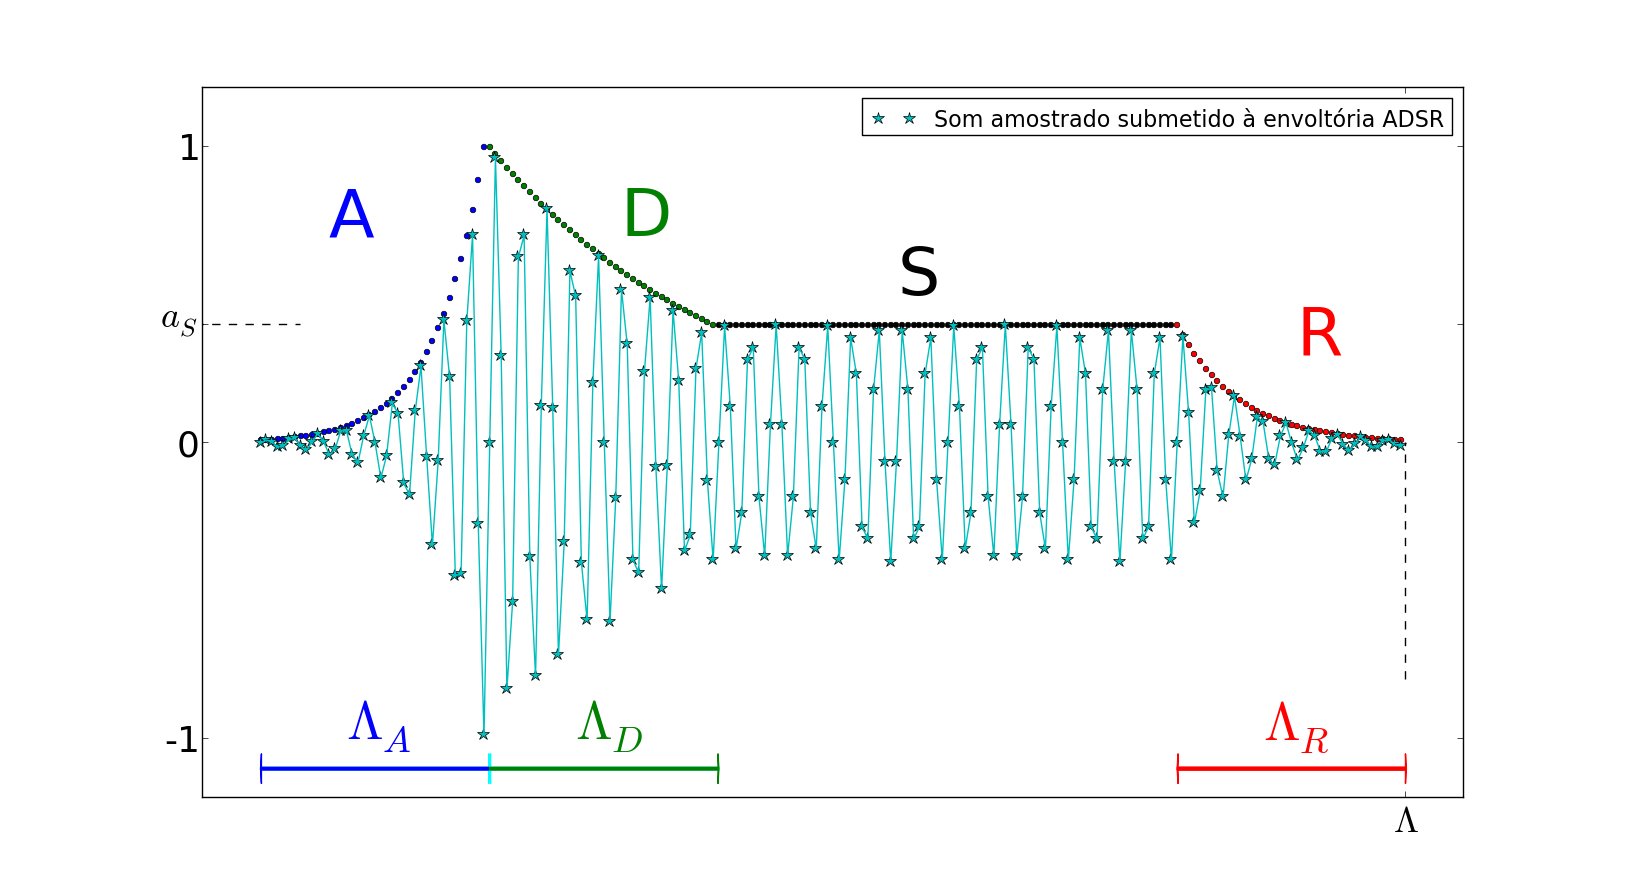
\includegraphics[width=\textwidth]{figuras/adsr}
        \label{fig:adsr}
\end{figure}


Podemos ver esquematicamente esta envoltória na figura~\ref{fig:adsr}. O envelope ADSR descrito é
uma implementação clássica e paradigmática que comporta variações diversas. Por exemplo,
entre o ataque e o decaimento, pode-se adicionar uma partição adicional em que a amplitude
máxima perdura. Outro exemplo comum é a elaboração de traçados mais elaborados para o
ataque ou para o decaimento.



\clearpage
\section{Organização de notas musicais em música}
Seja $ S_j=\{T_{i,1},T_{i,2}...T_{i,N}\} =\bigcup_{j \in [1,N]} T_{i,j} $ uma sequência de $N$ eventos
musicais. Para simplificar, sejam notas musicais estes eventos musicais.
Considerando $S$ uma estrutura musical, existem diversas técnicas
para tornar estas estruturas interessantes e agradáveis. 	

Os elementos de $S_j$ podem ser sobrepostos por mixagem (veja equação~\ref{eq:mixagem} e a figura~\ref{fig:mixagem}) formando intervalos e acordes ou concatenados (veja equação~\ref{eq:concatenacao} e a figura~\ref{fig:concatenacao}) formando sequências melódicas e rítmos.

\subsection{Afinação, intervalos, escalas e acordes}
Quando dobramos a frequência, temos uma oitava ascendente ($f=2f_0$).
Doze semitons equidistantes para o ouvido formam uma oitava,
portanto, se $f=2^{\frac{1}{12}}f_0$, temos um semitom entre $f_0$
e $f$.
O fator $\varepsilon=2^{\frac{1}{12}}$, equivalente a um semitom, forma uma grade de notas
no espectro audível, em que as frequências fundamentais possíveis
estão separadas por intervalos múltiplos de $\varepsilon$.
Esta precisão absoluta é característica de implementações
computacionais, pois os intrumentos reais possuem desvios destas frequências para melhor compatibilizar os harmônicos
de suas notas~\cite{Roederer}.

Esta divisão da oitava em doze notas é o cânone da música ocidental clássica,
além de usos cerimoniais/religiosos e étnicos~\cite{Wisnick}. Os intervalos entre quaisquer duas notas da escala de 12 notas em que se subdivide a oitava possuem nomes específicos. Notados em proporções de $\varepsilon$ entre as notas (i.e. um semitom), estes intervalos são, junto a suas notações abreviadas usuais:

\begin{equation}
\begin{split}
\text{uníssono} = 1J & = 0 \\
\text{semitom ou segunda menor} =2m & = 1 \\
\text{tom, tom inteiro ou segunda maior} =2M & = 2 \\
\text{terça menor} = 3m & = 3 \\
\text{terça maior} = 3M & = 4 \\
\text{quarta justa} = 4J & = 5 \\
\text{quarta aumentada, quinta diminuta ou trítono} = 4aum = 5dim = Tri & = 6 \\
\text{quinta justa} = 5J & = 7 \\
\text{sexta menor} = 6m & = 8 \\
\text{sexta maior} = 6M & = 9 \\
\text{sétima menor} = 7m & = 10 \\
\text{sétima maior} = 7M & = 11 \\
\text{oitava} = 8J & = 12
\end{split}
\end{equation}

Nesta nomenclatura (um dos padrões presentes no Brasil~\cite{Lacerda}),
um intervalo justo (uníssono, quarta, quinta e oitava), ou um intervalo maior (segunda maior, terça maior, sexta maior ou sétima maior), acrescido de um semitom, resulta em um intervalo aumentado. Um intervalo justo, ou um intervalo menor (segunda menor, terça menor, sexta menor ou sétima menor), decrescido de um semitom, resulta em um intervalo diminuto. Um intervalo maior, descrescido de um semitom,
resulta em um intervalo menor. Um intervalo menor, acrescido de um semitom, resulta em um intervalo maior. Um intervalo aumentado, acrescido de um semitom, resulta em um intervalo 'mais que aumentado' e um intervalo diminuto, descrescido de um semitom, resulta em um intervalo 'mais que diminuto'\footnote{A
 necessidade da nomenclatura, notação e uso de intervalos aumentados/diminutos e mais que aumentados/diminutos é consequência do sistema tonal, em que os graus da escala (veja abaixo) são realmente notas diferentes, com funções e usos específicos. Assim, em uma escala de dó bemol maior, a tônica - primeiro grau - é dó bemol, não si, e a sensível - sétimo grau - é si bemol, não lá sustenido ou dó duplo bemol.}. 

Caso as notas sejam dispostas sequencialmente, o intervalo é dito melódico. A ordem das notas, primeiro a nota mais grave ou a mais aguda, resulta em um intervalo ascendente ou descendente, respectivamente. 
Passando a nota mais grave para a oitava acima, ou a nota mais aguda uma oitava para baixo, invertemos o intervalo. Um pouco de exploração do sistema revela que um intervalo, somado à sua inversão, resulta 9. Um intervalo maior invertido resulta em um intervalo menor e vice-versa. Um intervalo aumentado invertido resulta diminuto e vice-versa, assim como o mais que aumentado resulta em mais que diminuto e vice-versa. Um intervalo justo invertido resulta igualmente justo.


Caso as notas soem simultaneamente, o intervalo é dito harmônico. Os intervalos de uníssono, oitava e quinta justa são consonâncias perfeitas. As terças e sextas são consideradas consonancias imperfeitas. As segundas, sétimas e trítonos são considerados dissonantes. Esta classificação não é absoluta. A discrepância mais comum é com relação à quarta justa, que é tida como consonante ou dissonante de acordo com o contexto e arcabouço teórico. Podemos considerá-la consonante sem muitos riscos. A sétima menor por vezes é considerada consonante, assim como algumas culturas entoam o trítono como intervalo consonante~\cite{Roederer,Wisnick}.

Um intervalo maior que a oitava é classificado como intervalo composto e leva o nome do intervalo entre as mesmas notas, mas na mesma oitava.

Este arcabouço resume com exatidão a teoria tradicional dos intervalos musicais~\cite{Lacerda} e nos será útil adiante. Dispomos esta nomenclatura também por completude desta exposição, não há necessidade alguma de decorar estes nomes ou apreender estes detalhes todos enquanto não há uso efetivo. A montagem \emph{Intervalos entre alturas} explora estes intervalos de formas isoladas e diversas.


Na escala cromática
de temperamento igual, temos 5 divisões perfeitamente simétricas, consideradas
escalas pelas simetrias internas e usos fáceis que disso resultam. Descrevamos
as escalas como sequências de inteiros aos quais $\varepsilon$ é elevado, resultando
nos fatores a serem multiplicados por $f_0$ para obtenção dos graus de cada escala:

\begin{equation}\label{escSim}
\begin{split}
\text{cromática} & = E_i^c = \{e_i^c\}_0^{11} =  \{0,1,2,3,4,5,6,7,8,9,10,11\} = \{i\}_0^{11}\\
\text{tons inteiros} & = E_i^t = \{e_i^t\}_0^{5} = \{0,2,4,6,8,10\} = \{2.i\}_0^{5} \\
\text{terças menores} & = E_i^{tm} = \{e_i^{tm}\}_0^{3} = \{0,3,6,9\} = \{3.i\}_0^3 \\
\text{terças maiores} & = E_i^{tM} = \{e_i^{tM}\}_0^{2} = \{0,4,8\} = \{4.i\}_0^2\\
\text{trítonos} & = E_i^{tt} = \{e_i^{tt}\}_0^{1} = \{ 0, 6 \} = \{6.i\}_0^1
\end{split}
\end{equation}

Assim, a terceira nota da escala em tons inteiros com $f_0=200Hz$
é $f_3=\varepsilon^{e_3^t} . f_0 = 2^{\frac{6}{12}} . 200 \approxeq 282.843 Hz$. Estas
'escalas' ou padrões, geram estruturas estáveis pelas simetrias internas, e podem ser
repetidas de forma eficiênte e sustentada. Discutiremos mais sobre simetrias e voltaremos
a estas divisões da oitava por igual. A montagem \emph{Cristais} expõe cada uma destas escalas tanto melódica quanto harmonicamente.

As escalas diatônicas também são facilmente especificadas, assim como
as escalas tonais maior e menor:


\begin{equation}
\begin{split}
\text{menor natural} = \text{modo eólico} & = E_i^m = \{e_i^m\}_0^6 = \{0,2,3,5,7,8,10\} \\
\text{modo lócrio} & = E_i^{mlo} = \{e_i^{mlo}\}_0^6 = \{0,1,3,5,6,8,10\} \\ 
\text{maior}  = \text{modo jônico} & = E_i^M = \{e_i^M\}_0^6 = \{0,2,4,5,7,9,11\} \\
\text{modo dórico} & = E_i^{md} = \{e_i^{md}\}_0^6 = \{0,2,3,5,7,9,10\} \\
\text{modo frígio} & = E_i^{mf} = \{e_i^{mf}\}_0^6 = \{0,1,3,5,7,8,10\} \\
\text{modo lídio} & = E_i^{ml}=\{e_i^{ml}\}_0^6 = \{0,2,4,6,7,9,11\} \\
\text{modo mixolídio} & = E_i^{mmi} = \{e_i^{mmi}\}_0^6 = \{0,2,4,5,7,9,10\}
\end{split}
\end{equation}

Observe que nas escalas diatônicas só estão presentes intervalos maiores, menores e justos dentre quaisquer duas notas escohidas. Única excessão para o trítono, que se apresenta como quarta aumenta ou quinta diminuta, dependendo da nota mais grave que se leva em consideração.

Todas as escalas diatônicas (salvo as menores harmônica e melódica)
seguem o padrão de intervalos sucessivos
tom, tom, semitom, tom, tom, tom, semitom. De forma
que podemos escrever:
\begin{equation}
\begin{split}
d_i & =\{2,2,1,2,2,2,1\} \\
e_0 & =0 \\
e_i & =d_{(i+\kappa)\%7}+e_{i-1} \quad para \;\;  i > 0
\end{split}
\end{equation}

Com $\kappa \in \mathbb{N}$. Para cada
modo, temos um único valor de $\kappa$ em qualquer intervalo $\in [x,x+6], \forall x \in \mathbb{N}$.


Por exemplo, consideremos o modo lídio. Uma breve
inspeção revela que $e_i^{ml}=d_{(i+2)\%7}+e_{i-1}^{ml}$. Temos, portanto, $\kappa=2$
para o modo lídio. 
Várias outras escalas e sequências são facilmente representadas desta forma. Em especial,
lembramos aqui das pentatônicas e os modos de transposição limitados de messiaen~\cite{Messiaen}.

A escala menor se apresenta em duas formas adicionais, dependentes do uso, melódico ou harmônico:

\begin{equation}
\begin{split}
\text{menor natural (igual acima)} & = E_i^m = \{e_i^m\}_0^6 = \{0,2,3,5,7,8,10\} \\
\text{menor harmônica} & = E_i^{mh} = \{e_i^{mh}\}_0^6 = \{0,2,3,5,7,8,11\} \\
\text{menor melódica} & = E_i^{mm} = \{e_i^{mm}\}_0^{14} = \{0,2,3,5,7,9,11,12,10,8,7,5,3,2,0\} \\
\end{split}
\end{equation}

e podem ser utilizadas livremente, embora tradicionamente se associem aos usos melódicos ou harmônicos sugeridos pelos seus nomes. Observe o traçado ascendente e descendente da escala menor melódica. Isso é necessário para que se apresente a sensível (sétimo e último grau separado por um semitom da oitava) no trajeto ascendente, o que não é necessário quando descende, retomando a forma natural. Já a harmônica apresenta a sensível, mas não evita o intervalo de segunda aumentada entre o sexto e sétimo graus, pois não precisa contemplar trajetória melódica, apenas apresentar a sensível tão cara ao sistema tonal~\cite{Harmonia}.

A ocorrência simultânea de notas é observada musicalmente em grande medida
através dos acordes. Destes, a base na musica tonal são as tríades, que consistem em duas terças sucessivas. Listamos os acordes triádicos sem inversão e na forma fechada\footnote{Um acorde invertido é aquele que apresenta no grave outra nota que não a fundamental. A posição fechada é aquela em que não cabe nota alguma do acorde entre quaisquer duas notas consecutivas~\cite{Lacerda}.},
com a fundamental em $0$:

\begin{equation}\label{triades}
\begin{split}
\text{tríade maior} = A_i^M= \{a_i^M\}_0^2=\{0,4,7\} \\ 
\text{tríade menor} = A_i^m = \{a_i^m\}_0^2=\{0,3,7\} \\
\text{tríade diminuta} = A_i^d = \{a_i^d\}_0^2=\{0,3,6\} \\
\text{tríade aumentada} = A_i^a = \{a_i^a\}_0^2=\{0,4,8\}
\end{split}
\end{equation}

Basta acrescentar $10$ ao final para ter o acorde (uma tétrade)
com sétima menor ou $11$ para resultar em sétima maior. As inversões e posições abertas
podem ser obtidas contando o número de semitons de cada nota a partir da nota mais grave.

Para a realização de microtonalidade\footnote{O uso explícito de
intervalos menores que o semitom é chamado microtonalismo. Isso pode ter usos
ornamentais ou estruturantes da música em si. A
divisão da oitava em $12$ notas igualmente espaçadas possui fundamentos físicos mas
não deixa de ser uma \emph{convenção}
(reconhecidamente adotada pela música erudita clássica de origem européia). Outras afinações
são também incidentes na manifestação musical humana, para citar somente um exemplo, a
música tradicional tailandesa utiliza uma divisão da oitava em sete notas igualmente
espaçadas ($\varepsilon=2^{\frac{1}{7}}$),
resultando em intervalos que pouco se assemelham aos intervalos presentes na
divisão de doze notas~\cite{Wisnick}.},
podemos usar reais não inteiros
para descrever a sequência de alturas ou modificar o fator $\varepsilon$
e usar inteiros ainda. Por exemplo, uma afinação muito
interessante por contemplar a série harmônica de forma consideravelmente precisa,
é proposta na forma da divisão da oitava em $53$ notas, de forma
que $\varepsilon=2^{\frac{1}{53}}$~\cite{microtonalidade}. As sequências de alturas
continuam sendo compostas por inteiros com o novo $\varepsilon$.
Note que se $S_i$ é uma sequência de alturas $s_i$ e mudamos de $\varepsilon_1$ para
$\varepsilon_2$,
resultamos em uma nova sequência $S_i'$ com $s_i'=s_i \frac{\varepsilon_1}{\varepsilon_2}$.


\subsection{Rudimentos de harmonia}

Abordaremos de forma bastante resumida e voltada para nossas aplicações
computacionais a harmonia tonal. Para harmonia modal e atonal recomendamos~\cite{harmEXT}.

Na chamada harmonia tradicional, as escalas maior e menor são usadas
de base para tríades feitas em cada grau da escala com duas terças consecutivas.
É conveniente, assim, notar os graus da escala pelos números da seguinte forma: $\hat{1},\hat{2},\hat{3},\hat{4},\hat{5},\hat{6},\hat{7}$.

Assim, as tríades formadas em cada grau é de fácil notação $\hat{1},\hat{3},\hat{5}$ é o acorde de primeiro grau, formado pelo primeiro grau da escala e central para uma música tonal. Em segundo lugar temos o acorde do quinto grau $\hat{5},\hat{7},\hat{2}$ ($\hat{7}$ sustenido no caso da escala menor) e em terceiro o do quarto grau $\hat{4},\hat{6},\hat{1}$. Depois consideramos as outras tríades todas. Ao longo da história, formas diferentes de lidar com estas tríades foram desenvolvidas. Estas convenções e técnicas apresentadas ao longo da história é o objeto de estudo da harmonia tradicional~\cite{Harmonia}.

A chamada harmonia funcional atribui funções a estes três acordes centrais e busca compreender seus usos através destas funções. O acorde formado sobre o primeiro grau é chamado de acorde de tônica e tem a função de manter um centro e um "chão" na música. O formado sobre o quinto grau é chamado de acorde de dominante e tem a função de tender à tônica, direcionar a música para ela. A tríade formada sobre o quarto grau é chamada de subdominante e tem a função de se distanciar da tônica.


A estes três acordes, são associadas as outras tríades. Na escala maior, a associada relativa (tônica relativa, subdominante relativa e dominante relativa) é a tríade formada uma terça abaixo e a associada anti-relativa (tônica anti-relativa, subdominante anti-relativa e a dominante anti-relativa) é a tríade formada na terça acima. Na escala menor ocorre o mesmo, mas a tríade a uma terça abaixo é chamada anti-relativa e a tríade a uma terça acima é chamada de relativa. As exatas funções e efeitos musicais destes acordes é motivo de bastante controvérsia. Dispomos da tabela~\ref{tab:harmonia} esta relação entre as tríades formadas em cada grau da escala.

\begin{table}[htpq!]
\centering
\begin{tabular}{l | c | r}
relativa & acorde principal da função & antirelativa \\\hline\hline
$\hat{6},\hat{1},\hat{3}$ & tônica:       $\hat{1},\hat{3},\hat{5}$ & $\hat{3}, \hat{5},      \hat{7}$ \\
$\hat{3},\hat{5},\hat{7}$ & dominante:    $\hat{5},\hat{7},\hat{2}$ & [ $\hat{7},\hat{2},\hat{4}\#$ ] \\
$\hat{2},\hat{4},\hat{6}$ & subdominante: $\hat{4},\hat{6},\hat{1}$ & $\hat{6},\hat{1},       \hat{3}$
\end{tabular}
\caption{Resumo das funções harmônicas tonais para escala maior}
\label{tab:harmonia}
\end{table}

Na escala menor, a relativa é a tríade iniciada uma terça acima e a antirelativa uma terça abaixo,
ou seja, se invertem com relação à tabela~\ref{tab:harmonia}. Outro detalhe destas tríades em modo
menor é a alteração do $\hat{7}$ um semitom acima para que fique somente a um semitom da tônica,
permitindo a dominante de fato (que deve ser maior e tender à tônica). Assim, a dominante é sempre maior, tanto em escalas maior ou menor. Por este motivo, a dominante relativa permanece a uma terça abaixo e a antirelativa a uma terça acima na escala menor.

A dominante anti-relativa forma um acorde menor, exigindo a alteração do quarto grau um semitom para cima $\hat{7}\#$. O acorde diminuto $\hat{7},\hat{2},\hat{4}$, geralmente é considerado uma 'dominante com sétima e sem fundamental'~\cite{Koellheuteur}.

Cada um destes acordes pode ser confirmado e se desenvolver com uma dominante e uma subdominante individuais (acorde com base na tríade formada a uma quinta acima e uma quinta abaixo respectivamente).

Por último, vale apontar as medianas\footnote{Também chamadas de medianas cromáticas.}, que são acordes formados também a uma terça, mas com alterações com relação ao acorde de origem. Caso haja duas alterações cromáticas, i.e. duas notas alteradas por um semitom cada com relação ao acorde original, a mediana é chamada 'duplamente cromática'. Esta relação entre acordes é considerada de tonalismo avançado, por vezes até de dissolução do tonalismo, e tem efeitos fortes e marcantes. Foi muito utilizada do final do romantismo em diante por Wagner, Lizt, Richard Strauss dentre outros e é bastante simples de ser realizada~\cite{Harmonia,Schachter}.

As modulações e sutilezas de encaminhamento de vozes podem ser encontradas em títulos diversos como os citados acima e constituem uma discussão longa e ainda presente. Apontamos somente que, para a condução de diferentes vozes, os movimentos que levam a notas vizinhas costumam soar mais coerentes, a importância maior da voz mais aguda e mais grave (e menor das vozes internas) e que as modulações se dão principalmente através de uma dominante individual que afirma a mudança da tônica e através de alterações cromáticas e enharmonias (mudança de função de um acorde). A importância da dominante torna ela o alvo primário e natural das modulações, resultando no circulo das quintas~\cite{Harmonia,Schachter,Koellheuteur,Harmony}.

A montagem musical \emph{Acorde cedo} explora estas relações entre acordes.

\subsection{Rudimentos de contraponto}

A condução de linhas melódicas simultâneas, chamadas vozes,
é matéria do campo de estudo chamado contraponto. A nossa bibliografia aponta títulos para estudos específicos, geralmente percorrendo formas sistemáticas de condução de vozes e desembocando em gêneros escolásticos como cânones, invenções e fugas. É possível resumir
as regras principais do contraponto e é dito que o próprio Beethoven - dentre outros - esboçou uma síntese.

Como
resumo de nossa bibliografia, apontamos que as dissonâncias só podem ser atingidas por movimento de
grau conjunto (notas vizinhas) ou resolvidas
imediatamente por movimento descendente de grau conjunto da voz superior. Além disso,
as consonâncias perfeitas só devem ser atacadas por movimento contrário ou oblíquo entre
as vozes. O movimento paralelo só é permitido entre consonâncias imperfeitas e não mais
do que 3 vezes consecutivas~\cite{Fux,Tragtenberg,SchoenbergContra}.
Estas regras tem como um dos objetivos principais, preservar a independência entre as vozes. Dispomos os movimentos tidos como base para o contraponto na figura~\ref{fig:movContraponto}. Observe o movimento paralelo como um caso específico do movimento oblíquo.


\begin{figure}[h!]
    \centering
    \caption{Movimentos diferenciados pelo contraponto}
        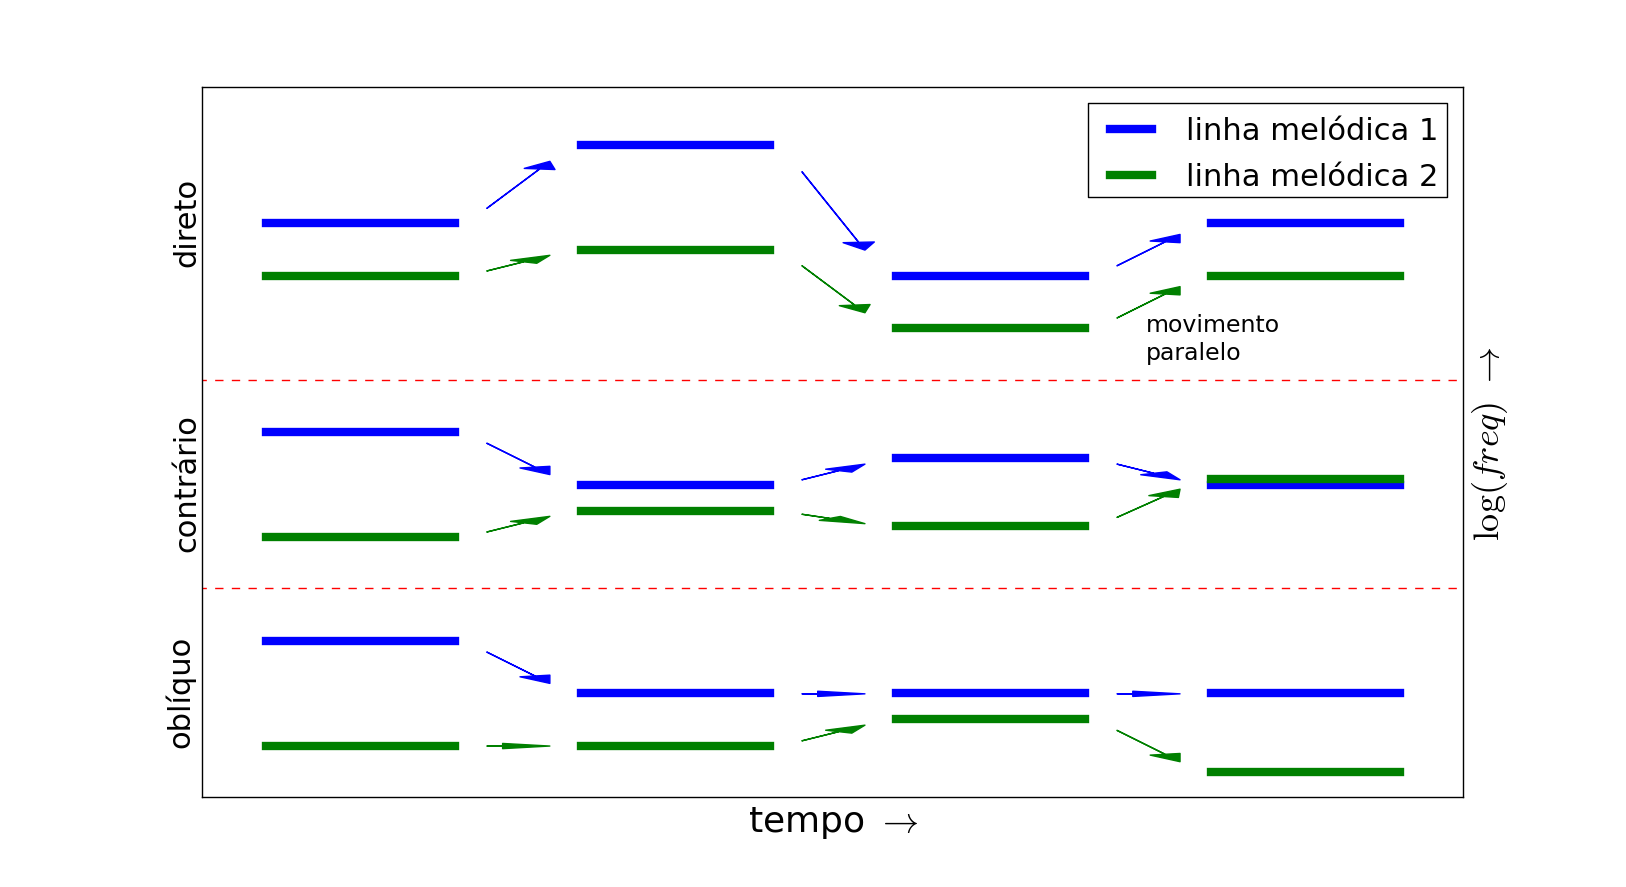
\includegraphics[width=\textwidth]{figuras/movContraponto}
        \label{fig:movContraponto}
\end{figure}




\subsection{Rítmo}
A noção rítmica é dependente de eventos separados por durações~\cite{rythm}. Estes eventos são discerníveis individualmente se separados
por ao menos $50-63ms$. Para que a separação entre eles possa ser apreciada, ela deve ser ainda um pouco maior,
por volta de $100ms$~\cite{microsound}. Podemos sumarizar 
a transição do domínio da apreciação
de durações como alturas para a apreciação em rítmo da seguinte forma ~\cite{Alfaix, microsound}:

\begin{center}
{\tiny 
\begin{tabular}{  l | r r r r   r r r    r r r || r r || r r r r r r }
\hline
           & \multicolumn{10}{c}{$\underleftarrow{\text{\bf zona de percepção de durações em rítmo}}$} & \multicolumn{2}{c}{transição} & \multicolumn{3}{c}{-} \\
duração (s) & {\bf ...}     & {\bf 32,}     & {\bf 16,}   & {\bf 8,}  & {\bf 4,}   & {\bf 2,}   & {\bf 1,}   & {\bf 1/2,} & {\bf 1/4,} & {\bf 1/8,} & $\frac{1}{16}=62,5ms$ , & $\frac{1}{20}=50ms$ & {\color{Gray} 1/40} & {\color{Gray} 1/80  } & {\color{Gray} 1/160 } & {\color{Gray} 1/320 } & {\color{Gray} 1/640 } & {\color{Gray} ... } \\
frequência (Hz) & {\color{Gray} ...} & {\color{Gray} 1/32,}   & {\color{Gray} 1/16,} & {\color{Gray} 1/8,} & {\color{Gray} 1/4,} & {\color{Gray} 1/2,} &  {\color{Gray} 1,}  & {\color{Gray} 2,}   & {\color{Gray} 4,}   & {\color{Gray} 8,}    & 16,  & 20   & {\bf 40}   & {\bf 80}   & {\bf 160}   & {\bf 320}   & {\bf 640}   & {\bf ...} \\
           & \multicolumn{10}{c}{ - } & \multicolumn{2}{c}{transição} & \multicolumn{6}{c}{$\overrightarrow{\text{\bf zona de percepção de durações em altura}}$} \\
\hline
%\ca
\end{tabular}
}
\end{center}

A banda de durações marcada como transição está minimizada pois os limites não são bem definidos: a duração específica em que começamos a perceber nitidademente uma frequência fundamental ou uma separação entre as ocorrências é dependente da pessoa e de características do som como conteúdo espectral e intensidade~\cite{microsound,Roederer}.

A métrica rítmica costuma se basear em uma duração básica chamada pulso. O pulso tipicamente
compreende durações entre $0.25-1.5s$ (respectivamente $240$ e $40BPM$). Na educação musical e estudos cognitivistas,
costuma-se associar esta gama de frequências de pulsação às durações entre batidas 
do coração ou entre os passos ao caminhar~\cite{Lacerda,Roederer}.

O pulso é subdividido em partes iguais e também é 
repetido sequencialmente. Estas relações (de divisão e de concatenação) costumam
seguir relações de números inteiros de baixa ordem
\footnote{Em ordem crescente de ocorrência na música
escrita e étnica, podemos
dizer que as divisões do pulso musical e seus agrupamentos
sequenciais no tempo ocorrem com fatores 2, 4 e 8, depois 3, 6 (dois grupos de 3 ou 3 grupos de 2) e 9 (3 grupos de 3). Por 
último os primos 5 e 7, completando 1-9.
Outras métricas são incidentes (divisões ou agrupamentos em 13, 17, etc), mas não são tão usuais e ocorrem principalmente em música experimental e erudita do século XX para frente. As métricas, por mais complexas que pareçam, costumam ser decompostas em divisões como estas~\cite{Gramani,Roederer}.}.
Uma exposição esquemática está na figura ~\ref{fig:pulsoSubAgl}.

\begin{figure}[h!]
    \centering
    \caption{Divisões e aglomerações do pulso musical para estabelecimento de métrica. Ao lado esquerdo temos as divisões da semínima estabelecida como pulso. Ao lado direito temos exemplos de fórmulas de compasso que especificam as mesmas métricas, mas na escala produzida pelas ocorrências e aglomerações do pulso musical.}
        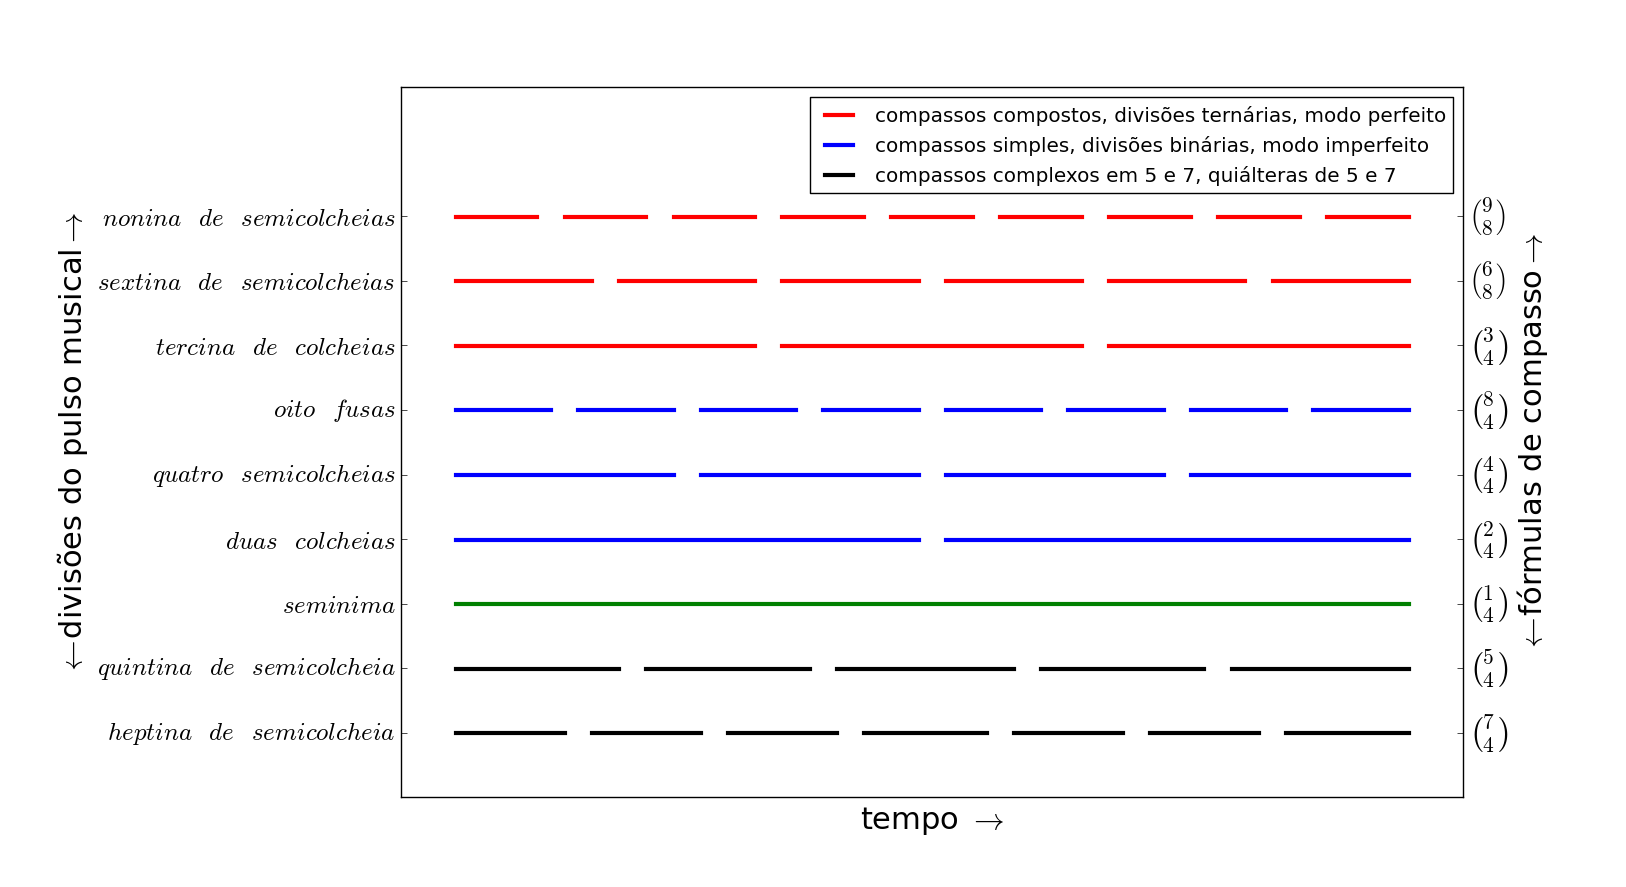
\includegraphics[width=\textwidth]{figuras/metricaMusical}
        \label{fig:pulsoSubAgl}
\end{figure}

As relações duais (compassos simples e divisões binárias) costumam a ocorrer em rítmos de dança
e ocasiões festivas e são chamadas imperfeitas. As relações triádicas
incidem mais na música ritualística e relacionada ao sagrado
e são ditas perfeitas.

As unidades mais fortes (acentuadas) são as que consistem nas 'cabeças das divisões'. A cabeça de um tempo ou uma unidade dividida é a primeira parte da subdivisão. Nas divisões binárias (2, 4 e 8 dos casos considerados aqui),
as unidades consideradas fortes se revesam com as fracas
(e.g. a divisão em 4 resulta em forte, fraco, (meio) forte, fraco).
Nas divisões ternárias (3, 6 e 9 dos casos considerados neste escrito)
à unidade forte (primeira) se sucedem 2 unidades fracas (e.g. a divisão em 3 resulta em forte, fraco fraco)\footnote{A divisão em 6 é considerada composta
 mas pode ocorrer também como uma divisão binária.
 Uma divisão binária que sofre então uma divisão ternária
 resulta em duas unidades divididas em três unidades cada: forte (subdividido em forte fraco, fraco) e fraco (subdividido em forte, fraco, fraco).
A outra forma de ocorrer a divisão em 6 é através de 
uma divisão ternária que sofre então uma divisão binária, resultando em:
uma unidade forte (subdividido em forte e fraco) e duas unidades fracas (subdivididas em forte e fraco cada).}.

A acentuação em tempos fracos é chamada contratempo, as notas que se iniciam em tempos fracos e cuja duração percorrem tempos fortes são as chamadas síncopas.

As notas podem ocorrer dentro e fora destas divisões (da \emph{'métrica musical'}). Nos casos mais comportados, as notas ocorrem exatamente nestas divisões, com maior incidência para ataques nos tempos fortes.
Em casos extremos, não se pode perceber a métrica~\cite{Roederer}. Variações (usualmente) bastante pequenas na grade compõem o que apreciamos como interpretação musical e diferenças entre estilos, junto a variações de intensidades, sobreposições de notas e timbre~\cite{Cook}.

Com o fim de sistematizar e colocar em termos formais, podemos convencionar
o pulso como nível $j=0$ de agrupamento, o nível $j=-1$ 
é a primeira subdivisão do pulso, o nível $j=1$ como a primeira algomeração dos pulsos e assim por diante. 

Desta forma, $P_i^j$ é a $i$-ésima unidade de 
pulsos no nível $j$ de agrupamento:
$P^0_{10}$ é o décimo pulso, $P^{1}_3$ é a terceira unidade de agrupamento de pulsos (possivelmente terceiro compasso),
$P^{-1}_2$ é a segunda unidade da subdivisão do pulso.

Especial atenção para
os limites de $j$ pois as divisões do pulso devem resultar em durações apreciáveis
como rítmo e também as junções do pulso devem resultar algo apreciável como, no máximo
do nosso escopo, uma música ou um conjunto coeso de músicas. Dito de outra forma: a duração de $P^{min(j)}_i$, para $\forall \; i$
é maior que $50ms$ e as durações de $P^{\text{máx}(j)}_i$ \emph{somadas}  em $\forall \; i$
devem resultar em uma duração menor do que alguns minutos ou, no máximo, poucas horas.


Para cada nível $j$ temos alguns índices $i$. Sempre que $i$ soma três 
(ou múltiplo de três) índices temos uma relação \emph{perfecta}, 
quando soma dois, quatro ou oito índices temos uma relação \emph{imperfecta} (veja figura~\ref{fig:pulsoSubAgl}.


Para especificar qualquer unidade (nota), de uma
dada sequência musical que tenha métrica,
podemos utilizar a notação:

\begin{equation}
P^{ \{ j_k \} }_{ \{ i_{k} \}}
\end{equation}

em que $j_k$ é o nível de aglomeração e $i_k$ é a ordem
da unidade em si.

Como um exemplo, podemos escrever $P^{-1,0,2}_{3,2,1}$  como a terceira subdivisão $P^{-1}_3$ do segundo
pulso $P^0_2$ do terceiro aglomerado de aglomerado de pulsos $P^2_2$ (perceba o termo $P^1_1$ omitido por simplicidade).

Cada unidade ou conjunto de unidades $P_i^j$ pode ser associada a uma sequência de amostras temporais $T_i$ que formam uma nota musical. 

Assim como acontece com outras características
musicais, lidamos com a estrutura rítmica sem fórmulas pre-estabelecidas, deixando procedimentos sistemáticos para quando é pertinente.


\subsection{Estruturas direcionais}

Dadas as estruturas musicais básicas tanto frequenciais (acordes e escalas) quanto 
rítmicas (divisões e aglomerações simples, compostas e complexas) é 
natural pensar em como realizar estas estruturas de forma que tenha coesão e sentido~\cite{Boulez}.

Neste ponto, encontramos alguns artifícios consagrados pelo tempo e pelo uso. 
Apresentamos aqui, de forma bastante breve, o pensamento musical dado por estruturas direcionais.
Na parte seguinte exploramos as estruturas recorrentes e cíclicas.

As estruturas direcionais nos possibiitam os recursos mais usuais: arcos melódicos e sequências que convergem ou divergem.

Os arcos melódicos são compostos por duas sequências convergentes: 
uma que atinge um ápice (chamado literalmente de clímax pela teoria musical tradicional) e 
outra que, de forma paradigmática, volta do ápice à região da nota de partida. Canonicamente, distinguimos entre arcos cujos clímax estão: no começo, no meio, no final, na primeira metade e na segunda metade~\cite{Schoenberg}. Dispomos esquematicamente a disposição destes clímax na figura~\ref{fig:climax}.

\begin{figure}[h!]
    \centering
    \caption{Distinções canônicas do clímax musical em uma melodia ou arcos em outras escalas}
        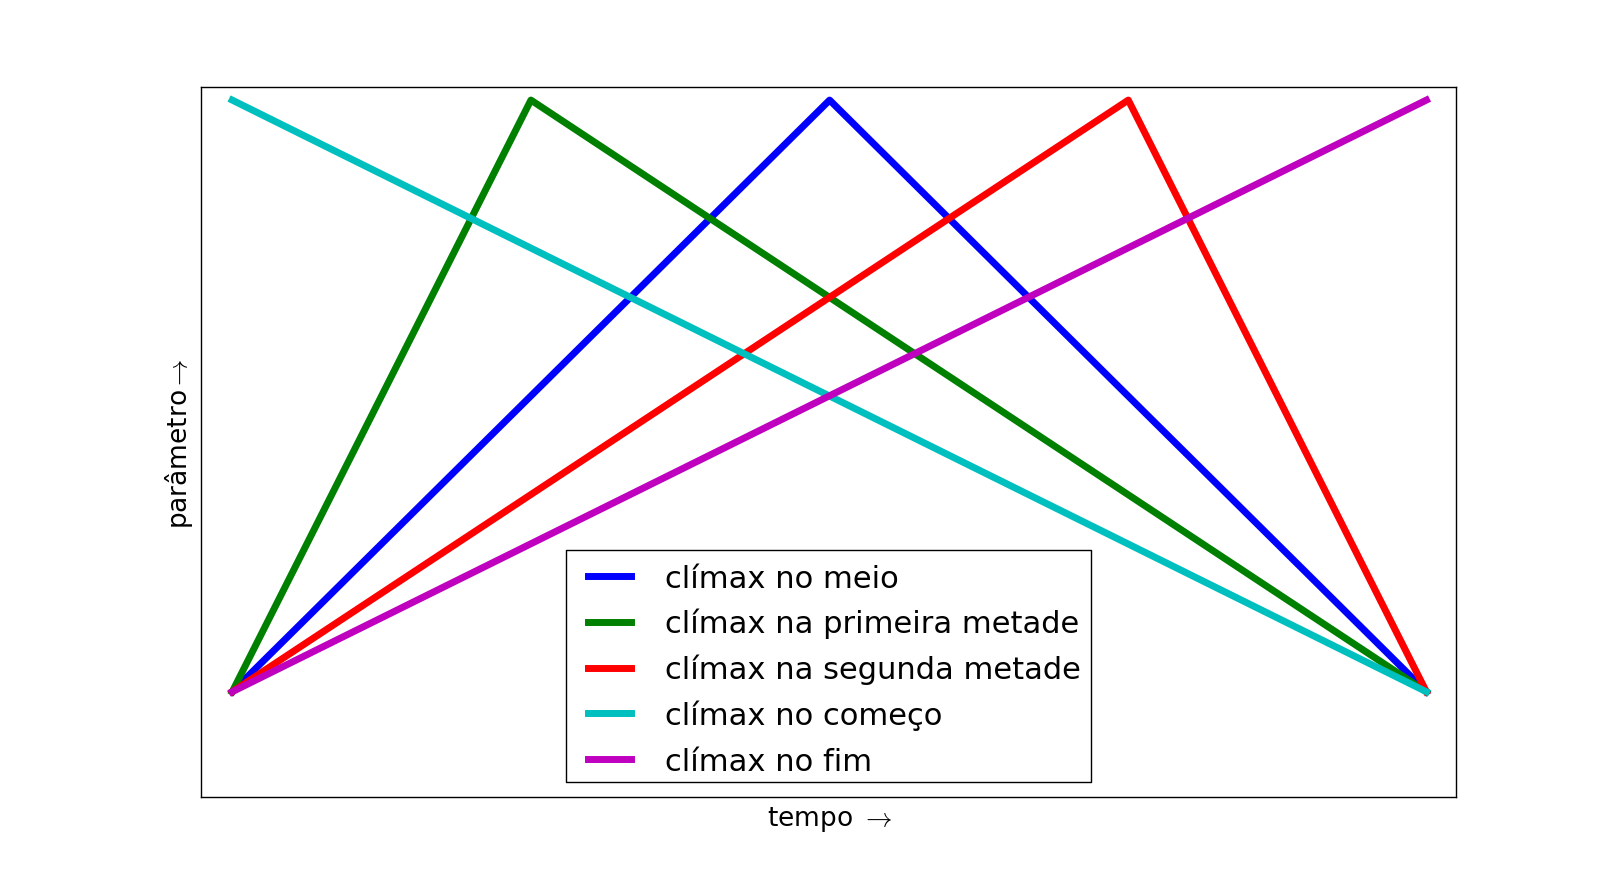
\includegraphics[width=\textwidth]{figuras/climax}
        \label{fig:climax}
\end{figure}


Seja $U_i=\{u_i\}_0^{\Lambda_U-1}$ uma sequência crescente. A sequência 
$R_i=\{r_i\}_0^{2\Lambda_U -2}=\{u_{(\Lambda_U-1-|\Lambda_U-1-i|)}\}_0^{2\Lambda_U-2}$ 
é uma sequência perfeitamente simétrica\footnote{Apresenta simetria especular perfeita, i.e. a segunda metade é uma versão espelhada da primeira.}. Pensada segundo conceitos musicais, o clímax está exatamente no meio da sequência. Podemos modificar isso fazendo com que alguma das metades seja expandida ou diminuída ou substituindo alguma das metades por outra sequência de tamanho diferente. É atraente este recurso pois contamos com toda a teoria de sequências, já bastante desenvolvida e estabelecida. Comparadas as sequências estudadas na teoria das sequências e as utilizadas na música, podemos concluir que existe um interesse especial por sequências relativamente curtas comparadas com as encontradas na teoria matemática~\cite{Guidorizzo,Schoenberg}. Teoricamente, estas sequências aplicadas a qualquer característica dos eventos musicais resulta em arcos. 
Assim, podemos conceber para a mesma sequência de eventos um certo número de arcos distintos, com tamanhos diferentes e climax diferentes para as características escolhidas. Embora este seja um recurso
bastante interessante e útil, vale manter em mente que a correlação dos arcos resulta em coerência da escuta~\cite{Schachter}.

\subsection{Estruturas cíclicas}\label{estCic}
Os arcos musicais nem sempre são fruto de estruturas direcionais como as citadas
acima. Um caso crítico é o de estruturas que se modificam gradualmente
até atingirem o estado original, formando um arco cíclico.

Neste caso, faremos uma exposição específica sobre permutações dada
a completude desta abordagem segundo princípios musicais, matemáticos e
filosóficos além da incidência musical histórica\footnote{De
forma bastante resumida, apontamos o
entendimento filosófico de que o pensamento humano se baseia
na percepção de semelhanças e diferenças dentre os estímulos
e objetos~\cite{Deleuze}. Portanto, segundo este entendimento,
as simetrias se encontram no cerne do processo cognitivo pois conceitualmente são as equivalências em si. Matematicamente,
as simetrias são representadas por grupos algébricos e os grupos finitos, por sua vez,
são sempre isomorfos a um grupo de permutações. Desta forma, podemos dizer que
as permutações são capazes de representar quaisquer simetrias em um sistema finito.
Diretamente na música encontramos permutações de forma bastante explícita, inclusive
na análise de música étnica~\cite{permMusic}.
Na tradição musical a permutação está presente em diversas técnicas~\cite{Zamacois} e
apontamos em especial a técnica \emph{Change Ringing} que consiste essencialmente
em padrões de permutações dentre um fixado número de notas~\cite{change}.} e a consequente realização de dois trabalhos acadêmicos~\cite{figgusOriginal, figgusEspacializacao}.

Qualquer conjunto de permutações pode ser utilizado como gerador de grupos algébricos~\cite{groups}. Assim, vale citarmos as propriedades que definem um grupo $G$:

\begin{equation}\label{eq:groups}
\begin{split}
\forall \;\; p_1,p_2 \in G \Rightarrow\quad\quad\quad\;\; p_1 \bullet p_2 & = p_3 \in G  \quad\quad\quad\;\;\;\text{(propriedade de fechamento)} \\
\forall \;\; p_1,p_2,p_3 \in G \Rightarrow\quad (p_1\bullet p_2)\bullet p_3 & = p_1\bullet (p_2\bullet p_3)\quad\;  \text{(propriedade da associatividade)} \\
\exists \;\; e \in G :\quad\quad\quad\quad\; p \bullet e & = e \bullet p \;\;\;\; \forall p \in G  \quad \text{(existência do elemento neutro)} \\
\forall \;\; p \in G, \;\exists\; p^{-1} :\quad\quad\quad\;  p\bullet p^{-1} & =p^{-1}\bullet p = e  \quad\quad\;\text{(existência do inverso)}
\end{split}
\end{equation}


A primeira destas propriedades nos é de particular importância, pois concluímos que toda permutação pode ser operada com outra permutação. De fato, podemos aplicar uma permutação, depois outra e, se compararmos com a ordenação inicial, temos uma permutação resultante. As outras propriedades resultam triviais para nosso caso.

Alguns teoremas nos são caros. Por exemplo, segue imediatamente que, em um grupo finito, todo elemento $p$ operado consigo mesmo um número suficiente de vezes resulta no elemento neutro $p^n=e$, pois caso contrário a propriedade do fechamento resultaria em um grupo infinito gerado por $p$. O menor $n\;:\;p^n=e$ é chamado de ordem do elemento. Assim, uma permutação finita $p$ aplicada sucessivamente um número suficiente de vezes resulta na ordenação inicial dos elementos, formando um ciclo, i.e. um arco musical se os elementos ordenados são elementos musicais e se consultados em cada estágio.

Estes arcos, que levam uma ordenação de elementos na mesma ordenação após um certo número de aplicações de permutações, podem ser efetuados pelo uso conjunto de diferentes permutações. Como exemplo
histórico, a tradição chamada \emph{change ringing} concebe música através de sinos tocados um após o outro e então tocados novamente, mas em uma ordem diferente. Este processo se repete até que se atinja a ordenação inicial e o conjunto de ordenações diferentes percorridas consiste no que é chamado de um \emph{peal}. Dispomos na tabela~\ref{tab:change} um \emph{peal} tradicional de 3 sinos (1, 2 e 3), que explora todas as suas ordenações. Cada linha apresenta uma ordenação dos sinos a ser tocada. As permutações agem aqui entre as linhas.
% {\color{blue} AA}

\begin{table}[htpq!]
\centering
\begin{tabular}{l c r}
\textcolor{red}{1} & \textcolor{blue}{2} & \textcolor{green}{3} \\
\textcolor{blue}{2} & \textcolor{red}{1} & \textcolor{green}{3} \\
\textcolor{blue}{2} & \textcolor{green}{3} & \textcolor{red}{1} \\
\textcolor{green}{3} & \textcolor{blue}{2} & \textcolor{red}{1} \\
\textcolor{green}{3} & \textcolor{red}{1} & \textcolor{blue}{2} \\
\textcolor{red}{1} & \textcolor{green}{3} & \textcolor{blue}{2} \\
\textcolor{red}{1} & \textcolor{blue}{2} & \textcolor{green}{3}
\end{tabular}
\caption{Change Ringing: \emph{Peal} (padrão) com 3 sinos}
\label{tab:change}
\end{table}

Para maiores detalhes desta tradição, recomendamos~\cite{change}. Importante para nós aqui é notar a existência de tradições musicais consciêntes da importância das permutações na música e observar que, neste caso, a estrutura musical consiste em permutações propriamente ditas e algumas permutações diferentes estão operando. 
Assim, fica claro o comportamento cíclico causado pela aplicação sucessiva da mesma permutação
e a consistência musical deste procedimento.

A utilização de permutações na música pode ser resumida da seguinte forma:
seja $L_i$ uma sequência de eventos musicais (para simplificar, considere
estes eventos como sendo notas musicais) e $p$ uma permutação.
$L_i'=p(L_i)$ consiste nos mesmos elementos de $L_i$ com a ordenação
modificada.

As permutações são usualmente escritas em notação cíclica ou natural. Por brevidade, vamos abordar somente a notação natural. Esta notação consiste na ordem dos índices originais considerados resultante da aplicação da permutação. Assim,
convencionada a ordenação original dada pela sequência de seus índices $[0\;1\;2\;3\;4\;5\;...]$ a permutação é notada pela sequência que produz (ex. $[1\;3\;7\;0\;...]$).

Importante notar que não é necessário permutar os elementos de $L_i$, mas somente
alguma ou algumas de suas características. Assim, seja $p^f$ uma permutação agindo
nas frequências e $L_i$ uma sequência de notas básicas como expostas
ao final de ~\ref{notaBasica}. A nova sequência $L_i'=p^f(L_i)$ consiste nas mesmas
notas musicais, na mesma ordem e com as mesmas características, com as frequências fundamentais permutadas segundo
o padrão que $p^f$ apresenta.

Por último, duas sutilezas deste procedimento.
Primeiro, a permutação $p$ não precisa envolver todos os elementos de $L_i$, i.e. ela
pode operar em subconjuntos de $L_i$. Segundo, nem todos os elementos $l_i$ precisam ser executados a
cada consulta de estado realizada.

Para simplificar, considere novamente os eventos de $L_i$ 
como notas musicais. Assim, se $i$ é vai de $0$ a $n$, e $n>4$, a cada compasso
de $4$ notas podemos executar somente as primeiras $4$ notas. As outras notas de
$L_i$ podem ser incidentes nos compassos em que as permutações aloquem
estas notas para as primeiras quatro notas de $L_i$.

Podemos dispor permutações que operem no mesmo conjunto, cada uma destas permutações
$p_i$ possui ao menos, segundo nossa exposição acima, vinculadas à permutação em si: dimensões das notas em que opera (frequência, duração, fades, intensidade, etc) e período de incidência (a cada quantas consultas é aplicada a permutação). Na realização das notas de $L_i$, uma solução fácil e coerente é executar as primeiras $n$ notas\footnote{A execução de notas disjuntas de $L_i$ equivale a modificar a permutação e executar as primeiras notas.}.

Esta abordagem resultou em alguns trabalhos~\cite{figgusOriginal,figgusEspacializacao} e implementações computacionais~\cite{repoFIGGUS,repoFIGGUSold}. Descrevemos um uso coerente desta técnica abaixo e apresentamos no APÊNCIDE~\ref{cap:FIGGUScode} a implementação computacional disponibilizada em~\cite{repoFIGGUS}

\subsection{Idioma musical?}

De certa forma central à experiência músical é a concepção de 'idioma musical'.
Existem diversas empreitadas para modelar e explorar diferentes entendimentos
sobre a linguagem musical e linguística aplicada à música e para discernimento entre 
o que seriam diferentes
'idiomas musicais'\cite{Lerdahl, Harmonia, Schachter,Alfaix}.

Apontamos aqui que, de forma simplificada e resumida, um idioma musical é fruto da
repetição de elementos e da repetição de relações entre elementos presentes no decorrer da música\footnote{A
música é tradicionalmente pensada através de dicotomias bastante relacionadas umas com as outras,
como: repetição e variação, relaxamento e tensão, equilíbrio e desequilíbrio, consonância e dissonância, etc}. 

\subsection{Usos musicais}

Primeiro, a nota básica foi definida e suas características postas em termos
claros e quantitativos (sessão~\ref{notaBasica}). Em seguida, adentramos a nota musical e suas transições internas,
além de tratamentos imediatos (sessão~\ref{varInternas}). Por fim, nesta última sessão, apresentamos
recursos consagrados para organizar estas notas musicais em música.

Assim, atingimos uma gama de recursos com uma infinidade de possibilidades de resultados,
situação típica e tão cara às artes~\cite{Harmonia,Webern}.

Existem explorações e estudos individuais para cada recurso apresentado. Por exemplo, pode-se obter as harmonias triádicas 'sujas' (com notas não pertencentes à tríade) através de sobreposições de quartas justas. Outro exemplo interessante é a presença simultânea de rítmos em diferentes métricas, constituindo o que chamamos de \emph{polirritmia}. A montagem musical \emph{Poli-hit mia} explora estas métricas simultâneas através de trem de impulsos convoluídos com as notas que compõem cada linha.

As escalas microtonais são bastante importantes na música do século XX~\cite{microtonalidade} e possuem vários usos com resultados muito marcantes, como os usos de quartos de tom na música indiana e possibilidades de batimentos. A sequência musical \emph{MicroTom} explora estes recursos de forma explícita, incluindo melodias microtonais e harmonias microtonais com várias notas em um âmbito de alturas bastante reduzido.

Novamente, vínculos entre parâmetros são formas poderosas de resultar músicas ou ao menos montagens musicais. O número de notas permutadas podem variar no decorrer da música, revelando vínculo com a duração da peça. As harmonias podem consituir-se triádicas (eqs.~\ref{triades}) com notas replicadas em várias oitavas e mais numerosas quanto menor a profundidade e frequência de vibratos (eqs.~\ref{vbrGamma},~\ref{vbrAux},~\ref{vbrF},~\ref{vbrGamma2},~\ref{vbrT}), dentre outras incontáveis possibilidades.

Um uso particularmente coerente, do ponto de vista das simetrias apresentadas nas divisões da oitava (eqs.~\ref{escSim}) e das simetrias apresentadas através das permutações (tabela~\ref{tab:change} e eqs.~\ref{eq:groups}) é o uso conjunto de ambos. Nas peças \emph{3 trios} esta associação é feita de forma sistemática para possibilitar uma audição dedicada a esta associação.

O \emph{PPEPPS} (Pure Python EP: Projeto Solvente) é um EP inteiro sintetizado com os recursos apresentados neste trabalho. Com pouca parametrização, o programa resulta músicas inteiras, permitindo a composição de músicas e conjuntos de músicas com facilidade. As possibilidades de compartilhamento envolvem obter este album (ou outro feito de forma semelhante) baixando algumas linhas de código e rodando para obter uma pasta com as músicas.


